% latex-mimosis has been used as the thesis template
% https://github.com/Pseudomanifold/latex-mimosis
% Which is under the following LICENSE:

% Copyright (c) 2018 Bastian Rieck
% 
% Permission is hereby granted, free of charge, to any person obtaining a copy
% of this software and associated documentation files (the "Software"), to deal
% in the Software without restriction, including without limitation the rights
% to use, copy, modify, merge, publish, distribute, sublicense, and/or sell
% copies of the Software, and to permit persons to whom the Software is
% furnished to do so, subject to the following conditions:
% 
% The above copyright notice and this permission notice shall be included in all
% copies or substantial portions of the Software.
% 
% THE SOFTWARE IS PROVIDED "AS IS", WITHOUT WARRANTY OF ANY KIND, EXPRESS OR
% IMPLIED, INCLUDING BUT NOT LIMITED TO THE WARRANTIES OF MERCHANTABILITY,
% FITNESS FOR A PARTICULAR PURPOSE AND NONINFRINGEMENT. IN NO EVENT SHALL THE
% AUTHORS OR COPYRIGHT HOLDERS BE LIABLE FOR ANY CLAIM, DAMAGES OR OTHER
% LIABILITY, WHETHER IN AN ACTION OF CONTRACT, TORT OR OTHERWISE, ARISING FROM,
% OUT OF OR IN CONNECTION WITH THE SOFTWARE OR THE USE OR OTHER DEALINGS IN THE
% SOFTWARE.
\documentclass{mimosis}

\usepackage{metalogo}

\emergencystretch=1em % overfull hboxes of bibliography

%%%%%%%%%%%%%%%%%%%%%%%%%%%%%%%%%%%%%%%%%%%%%%%%%%%%%%%%%%%%%%%%%%%%%%%%
% Some of my favourite personal adjustments
%%%%%%%%%%%%%%%%%%%%%%%%%%%%%%%%%%%%%%%%%%%%%%%%%%%%%%%%%%%%%%%%%%%%%%%%
%
% These are the adjustments that I consider necessary for typesetting
% a nice thesis. However, they are *not* included in the template, as
% I do not want to force you to use them.

% This ensures that I am able to typeset bold font in table while still aligning the numbers
% correctly.
\usepackage{etoolbox}

\usepackage[binary-units=true]{siunitx}
\DeclareSIUnit\px{px}

\sisetup{%
  detect-all           = true,
  detect-family        = true,
  detect-mode          = true,
  detect-shape         = true,
  detect-weight        = true,
  detect-inline-weight = math,
}

%%%%%%%%%%%%%%%%%%%%%%%%%%%%%%%%%%%%%%%%%%%%%%%%%%%%%%%%%%%%%%%%%%%%%%%%
% Hyperlinks & bookmarks
%%%%%%%%%%%%%%%%%%%%%%%%%%%%%%%%%%%%%%%%%%%%%%%%%%%%%%%%%%%%%%%%%%%%%%%%

\usepackage[%
  colorlinks = true,
  %colorlinks = false, % for printing
  citecolor  = RoyalBlue,
  linkcolor  = RoyalBlue,
  urlcolor   = RoyalBlue,
  unicode,
  ]{hyperref}

\usepackage{bookmark}

%%%%%%%%%%%%%%%%%%%%%%%%%%%%%%%%%%%%%%%%%%%%%%%%%%%%%%%%%%%%%%%%%%%%%%%%
% Bibliography
%%%%%%%%%%%%%%%%%%%%%%%%%%%%%%%%%%%%%%%%%%%%%%%%%%%%%%%%%%%%%%%%%%%%%%%%
%
% I like the bibliography to be extremely plain, showing only a numeric
% identifier and citing everything in simple brackets. The first names,
% if present, will be initialized. DOIs and URLs will be preserved.

\usepackage[%
  autocite     = plain,
  backend      = biber,
  doi          = true,
  url          = true,
  giveninits   = true,
  hyperref     = true,
  maxbibnames  = 99,
  maxcitenames = 99,
  sorting      = none, % sort by appareance
  style        = numeric,
  ]{biblatex}

% Copyright (c) 2018 Bastian Rieck
% 
% Permission is hereby granted, free of charge, to any person obtaining a copy
% of this software and associated documentation files (the "Software"), to deal
% in the Software without restriction, including without limitation the rights
% to use, copy, modify, merge, publish, distribute, sublicense, and/or sell
% copies of the Software, and to permit persons to whom the Software is
% furnished to do so, subject to the following conditions:
% 
% The above copyright notice and this permission notice shall be included in all
% copies or substantial portions of the Software.
% 
% THE SOFTWARE IS PROVIDED "AS IS", WITHOUT WARRANTY OF ANY KIND, EXPRESS OR
% IMPLIED, INCLUDING BUT NOT LIMITED TO THE WARRANTIES OF MERCHANTABILITY,
% FITNESS FOR A PARTICULAR PURPOSE AND NONINFRINGEMENT. IN NO EVENT SHALL THE
% AUTHORS OR COPYRIGHT HOLDERS BE LIABLE FOR ANY CLAIM, DAMAGES OR OTHER
% LIABILITY, WHETHER IN AN ACTION OF CONTRACT, TORT OR OTHERWISE, ARISING FROM,
% OUT OF OR IN CONNECTION WITH THE SOFTWARE OR THE USE OR OTHER DEALINGS IN THE
% SOFTWARE.


%%%%%%%%%%%%%%%%%%%%%%%%%%%%%%%%%%%%%%%%%%%%%%%%%%%%%%%%%%%%%%%%%%%%%%%%
% Some adjustments to make the bibliography more clean
%%%%%%%%%%%%%%%%%%%%%%%%%%%%%%%%%%%%%%%%%%%%%%%%%%%%%%%%%%%%%%%%%%%%%%%%
%
% The subsequent commands do the following:
%  - Removing the month field from the bibliography
%  - Fixing the Oxford commma
%  - Suppress the "in" for journal articles
%  - Remove the parentheses of the year in an article
%  - Delimit volume and issue of an article by a colon ":" instead of
%    a dot ""
%  - Use commas to separate the location of publishers from their name
%  - Remove the abbreviation for technical reports
%  - Display the label of bibliographic entries without brackets in the
%    bibliography
%  - Ensure that DOIs are followed by a non-breakable space
%  - Use hair spaces between initials of authors
%  - Make the font size of citations smaller
%  - Fixing ordinal numbers (1st, 2nd, 3rd, and so) on by using
%    superscripts

% Remove the month field from the bibliography. It does not serve a good
% purpose, I guess. And often, it cannot be used because the journals
% have some crazy issue policies.
\AtEveryBibitem{\clearfield{month}}
\AtEveryCitekey{\clearfield{month}}

% Fixing the Oxford comma. Not sure whether this is the proper solution.
% More information is available under [1] and [2].
%
% [1] http://tex.stackexchange.com/questions/97712/biblatex-apa-style-is-missing-a-comma-in-the-references-why
% [2] http://tex.stackexchange.com/questions/44048/use-et-al-in-biblatex-custom-style
%
\AtBeginBibliography{%
  \renewcommand*{\finalnamedelim}{%
    \ifthenelse{\value{listcount} > 2}{%
      \addcomma
      \addspace
      \bibstring{and}%
    }{%
      \addspace
      \bibstring{and}%
    }
  }
}

% Suppress "in" for journal articles. This is unnecessary in my opinion
% because the journal title is typeset in italics anyway.
\renewbibmacro{in:}{%
  \ifentrytype{article}
  {%
  }%
  % else
  {%
    \printtext{\bibstring{in}\intitlepunct}%
  }%
}

% Remove the parentheses for the year in an article. This removes a lot
% of undesired parentheses in the bibliography, thereby improving the
% readability. Moreover, it makes the look of the bibliography more
% consistent.
\renewbibmacro*{issue+date}{%
  \setunit{\addcomma\space}
    \iffieldundef{issue}
      {\usebibmacro{date}}
      {\printfield{issue}%
       \setunit*{\addspace}%
       \usebibmacro{date}}%
  \newunit}

% Delimit the volume and the number of an article by a colon instead of
% by a dot, which I consider to be more readable.
\renewbibmacro*{volume+number+eid}{%
  \printfield{volume}%
  \setunit*{\addcolon}%
  \printfield{number}%
  \setunit{\addcomma\space}%
  \printfield{eid}%
}

% Do not use a colon for the publisher location. Instead, connect
% publisher, location, and date via commas.
\renewbibmacro*{publisher+location+date}{%
  \printlist{publisher}%
  \setunit*{\addcomma\space}%
  \printlist{location}%
  \setunit*{\addcomma\space}%
  \usebibmacro{date}%
  \newunit%
}

% Ditto for other entry types.
\renewbibmacro*{organization+location+date}{%
  \printlist{location}%
  \setunit*{\addcomma\space}%
  \printlist{organization}%
  \setunit*{\addcomma\space}%
  \usebibmacro{date}%
  \newunit%
}

% Display the label of a bibliographic entry in bare style, without any
% brackets. I like this more than the default.
%
% Note that this is *really* the proper and official way of doing this.
\DeclareFieldFormat{labelnumberwidth}{#1\adddot}

% Ensure that DOIs are followed by a non-breakable space.
\DeclareFieldFormat{doi}{%
  \mkbibacro{DOI}\addcolon\addnbspace
    \ifhyperref
      {\href{http://dx.doi.org/#1}{\nolinkurl{#1}}}
      %
      {\nolinkurl{#1}}
}

% Use proper hair spaces between initials as suggested by Bringhurst and
% others.
\renewcommand*\bibinitdelim {\addnbthinspace}
\renewcommand*\bibnamedelima{\addnbthinspace}
\renewcommand*\bibnamedelimb{\addnbthinspace}
\renewcommand*\bibnamedelimi{\addnbthinspace}

% Make the font size of citations smaller. Depending on your selected
% font, you might not need this.
\renewcommand*{\citesetup}{%
  \biburlsetup
  \small
}

\DeclareLanguageMapping{english}{english-mimosis}

\addbibresource{Thesis.bib}

%%%%%%%%%%%%%%%%%%%%%%%%%%%%%%%%%%%%%%%%%%%%%%%%%%%%%%%%%%%%%%%%%%%%%%%%
% Fonts
%%%%%%%%%%%%%%%%%%%%%%%%%%%%%%%%%%%%%%%%%%%%%%%%%%%%%%%%%%%%%%%%%%%%%%%%

\ifxetexorluatex
  \setmainfont{Minion Pro}
\else
  \usepackage[lf]{ebgaramond}
  \usepackage[oldstyle,scale=0.7]{sourcecodepro}
  \singlespacing
\fi

\renewcommand{\th}{\textsuperscript{\textup{th}}\xspace}

\makeindex
\makeglossaries

%%%%%%%%%%%%%%%%%%%%%%%%%%%%%%%%%%%%%%%%%%%%%%%%%%%%%%%%%%%%%%%%%%%%%%%%
% Incipit
%%%%%%%%%%%%%%%%%%%%%%%%%%%%%%%%%%%%%%%%%%%%%%%%%%%%%%%%%%%%%%%%%%%%%%%%

\usepackage{enumerate} % List of steps
\usepackage{placeins} % Floatbarrier

%subfigures
\usepackage{caption}
\usepackage{subcaption}

\usepackage{svg} % to include SVGs
\usepackage{pdfpages} % to include PDFs (title)

% custom commands
\newcommand{\q}[1]{``#1''} % quote command
\newcommand{\monosp}[1]{$#1$} % monospace math
\newcommand{\monobold}[1]{\pmb{#1}} % monospace math bold



%% DOCUMENT START

\begin{document}


% HEADINGS

\frontmatter
  \begin{titlepage}
    
\includepdf[pages=-]{title.pdf}
\end{titlepage}

\newpage
\null
\thispagestyle{empty}
\newpage

  \begin{center}
  \textsc{Abstract}
\end{center}
%
\noindent
% CONTEXT
Skin detection is the process of discriminating skin and non-skin pixels in an arbitrary image and represents an intermediate step in several image processing tasks, such as facial analysis and biomedical segmentation.
% PROBLEM to overcome
Different approaches have been presented in the literature, but a comparison is difficult to perform due to multiple datasets and varying performance measurements.
% HOW i addressed it
In this work, the datasets and the state-of-the-art approaches are reviewed and categorized using a new proposed taxonomy.
% WHAT i have done
Three different representative skin detector methods of the state of the art are selected and thoroughly analyzed. This approaches are then evaluated on three different state of the art datasets and skin tones sub-datasets using multiple metrics.
The evaluation is performed on single and cross dataset scenario to highlight key differences between methods, reporting also the inference time.
Finally, the results are organized into multiple tables, using the related figures as an assistance tool to support the discussion. %to exhibit meaningful instances.
% KEY IMPACT of the work
Experimental results demonstrate the strength and weaknesses of each approach, and the need to involve multiple metrics for a fair assessment of the method's aspects.

  \begin{center}
  \textsc{Acknowledgments}
\end{center}
%
\noindent
%
The journey of completing my Bachelor's degree and writing this thesis has been demanding in many respects.\\
Nevertheless, it has been one of the most enriching experiences I've ever had and now that it comes to an end, I want to thank the people who supported me and helped me through it.

\vspace{2mm}
I would like to thank Prof. Raimondo Schettini for giving me the opportunity of working on this project.\\
This thesis has allowed me to explore fields that otherwise would have been difficult to encounter and that have fascinated me greatly.

\vspace{2mm}
I would like to extend my deepest gratitude to Dr. Mirko Agarla whose invaluable assistance and patience helped me in every step of the way.\\
I must also thank him for the much needed critical advice on the writing of this thesis.

\vspace{2mm}
I am grateful to my family for supporting me throughout the entire duration of my studies.



  \tableofcontents


% CONTENT

\mainmatter

  %%%%%%%%%%%%%%%%%%%%%%%%%%%%%%%%%%%%%%%%%%%%%%%%%%%%%%%%%%%%%%%%%%%%%%%%
\chapter{Introduction}\label{chap:introduction}
%%%%%%%%%%%%%%%%%%%%%%%%%%%%%%%%%%%%%%%%%%%%%%%%%%%%%%%%%%%%%%%%%%%%%%%%


\noindent The presence of human skin in media gives meaningful information. 
Skin features are important cues that can be used to infer a variety of aspects related to a person, such as attractiveness, age, and health~\cite{fink2006visible, choi2011age}.
Skin detection is the process of discriminating skin and non-skin pixels in an arbitrary image or video, as illustrated in \autoref{fig:skin-detection}. It is primarily used as an intermediate step for more complex tasks such as facial analysis~\cite{ramirez2014color, baskan2002projection}, gesture analysis~\cite{singha2018dynamic}, video surveillance~\cite{chen2012statistical}, privacy protection~\cite{shifa2020skin}, adult image detection~\cite{jones2002statistical, stottinger2009skin, zhu2004adaptive}, region-of-interest detection~\cite{liu2008region}, and advertisements~\cite{low2020multi}.
In the biomedical field, skin detection plays an important role in lesions segmentation and cutaneous diseases classification~\cite{do2014early, ronneberger2015u}.
Detecting skin-colored pixels has proven quite challenging for various reasons.
Materials with a similar color to the skin, such as wood, copper, leather, and sand, can be incorrectly labeled as skin pixels.
Moreover, the appearance of skin in an image depends on many variables, such as the illumination conditions, the camera color science, and motion blur~\cite{zarit1999comparison}.
Finally, skin tones vary dramatically within and across individuals.
Some challenging aspects are depicted in \autoref{fig:common-issues}.

\begin{figure}[hb]
     \centering
     \begin{subfigure}[b]{0.45\textwidth}
         \centering
         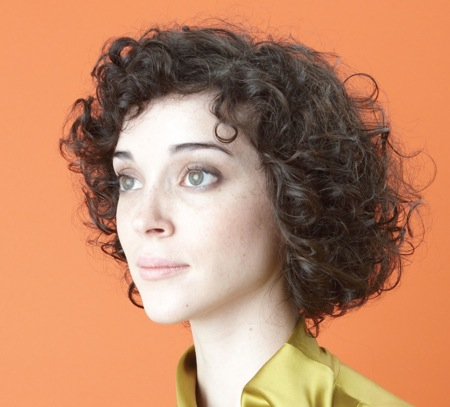
\includegraphics[width=\textwidth]{images/introduction/skin_det_ori3.jpg}
         \caption{}
         \label{fig:skin-detection-ori}
     \end{subfigure}
     \hfill
     \begin{subfigure}[b]{0.45\textwidth}
         \centering
         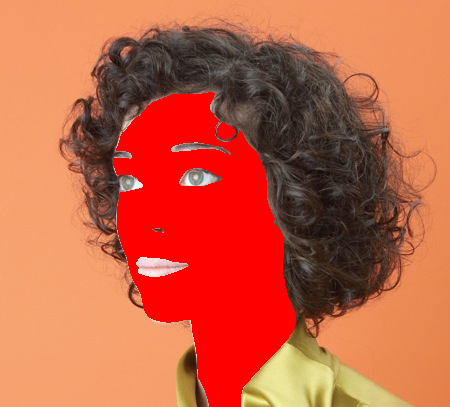
\includegraphics[width=\textwidth]{images/introduction/skin_det_red3.png}
         \caption{}
         \label{fig:skin-detection-red}
     \end{subfigure}
        \caption{Skin detection: (a) original image; (b) detected skin pixels. The original image is part of the Pratheepan dataset~\cite{tan2011fusion}.}
        \label{fig:skin-detection}
\end{figure}

\begin{figure}[h]
     \centering
     \begin{subfigure}[b]{0.3\textwidth}
         \centering
         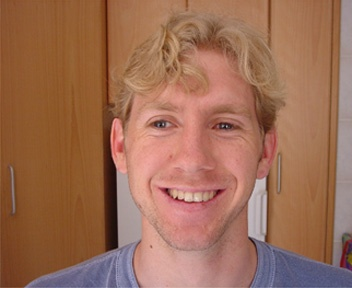
\includegraphics[width=\textwidth]{images/introduction/im00060x.jpg}
         \label{fig:thresh-wood-x}
     \end{subfigure}
     \hfill
     \begin{subfigure}[b]{0.3\textwidth}
         \centering
         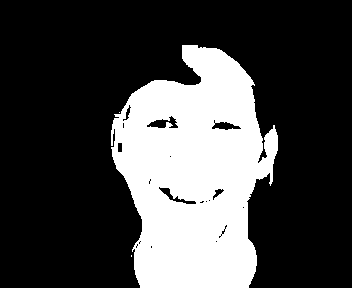
\includegraphics[width=\textwidth]{images/introduction/im00060y.png}
         \label{fig:thresh-wood-y}
     \end{subfigure}
    \hfill
     \begin{subfigure}[b]{0.3\textwidth}
         \centering
         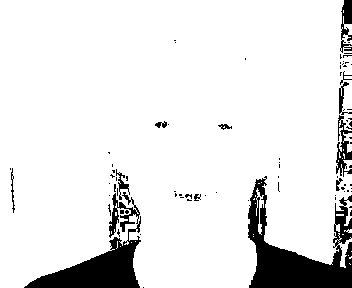
\includegraphics[width=\textwidth]{images/introduction/im00060p.png}
         \label{fig:thresh-wood-p}
     \end{subfigure}
     \begin{subfigure}[b]{0.3\textwidth}
         \centering
         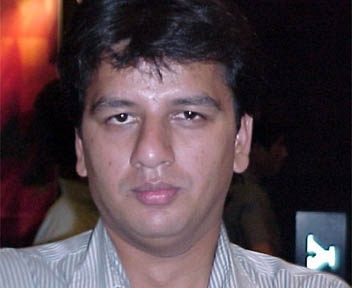
\includegraphics[width=\textwidth]{images/introduction/im00081x.jpg}
         \caption{}
         \label{fig:thresh-color-x}
     \end{subfigure}
     \hfill
     \begin{subfigure}[b]{0.3\textwidth}
         \centering
         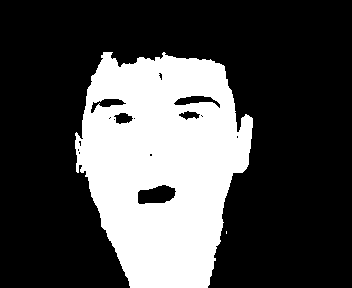
\includegraphics[width=\textwidth]{images/introduction/im00081y.png}
         \caption{}
         \label{fig:thresh-color-y}
     \end{subfigure}
     \hfill
     \begin{subfigure}[b]{0.3\textwidth}
         \centering
         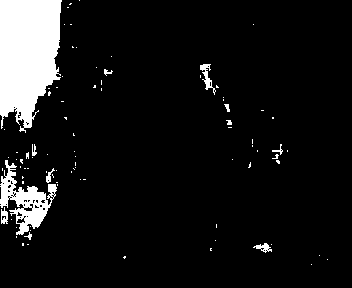
\includegraphics[width=\textwidth]{images/introduction/im00081p.png}
         \caption{}
         \label{fig:thresh-color-p}
     \end{subfigure}
        \caption{Challenges of skin detection, visualized through: (a) the input image, (b) the ground truth, (c) the prediction obtained from a thresholding method~\cite{brancati2017human}.
        The first row depicts an image containing materials with skin-like colors. The second row shows how the colors of an image can be affected by the illumination conditions.}
        \label{fig:common-issues}
\end{figure}

This thesis presents a review of the skin detection datasets and state-of-the-art approaches.
Image databases and state-of-the-art approaches are retrieved, and a new taxonomy is proposed.
Three different computational approaches are selected, thoroughly analyzed, and implemented to compare their strength, weaknesses, generalization capability, and performance.
Before assessing the methods, a validation phase takes place; then the methods are evaluated in single and cross dataset settings over three datasets and three skin tones sub-datasets, using multiple metrics.
Finally, inference times are compared.

The main contributions of this work are the following:
\begin{itemize}
  \item A comparative review of common datasets used in skin detection and discussion on some major data limitations.
  \item An analysis of the state-of-the-art approaches at skin detection, with the proposal for a new taxonomy.
  \item An analysis of some of the evaluation metrics used in binary classification problems.
  \item An in-depth analysis of the three representative state-of-the-art approaches.
  \item An evaluation of the selected approaches on three public datasets in single-dataset and cross-dataset settings.
  \item An evaluation of the selected approaches on three skin tones sub-datasets in single-dataset and cross-dataset settings.
  \item An evaluation of the inferences times of the selected approaches.
\end{itemize}
The thesis is organized as follows: the Chapter \ref{chap:datasets} gives an overview of the datasets used in skin detection including a discussion on the limitations and a detailed description of the three chosen datasets.
Chapter \ref{chap:methods} contains an in-depth analysis of the selected approaches, describing the architecture, functioning, and operations performed by each method.
Chapter \ref{chap:results} contains a detailed explanation of the experiments setup and the evaluation process.
Then, the evaluation results are presented and extensively commented.
Finally, Chapter \ref{chap:conclusion} draws conclusions and gives an outlook on possible future work.

%%%%%%%%%%%%%%%%%%%%%%%%%%%%%%%%%%%%%%%%%%%%%%%%%%%%%%%%%%%%%%%%%%%%%%%%
\section{State of the art}\label{sec:state-of-the-art}
%%%%%%%%%%%%%%%%%%%%%%%%%%%%%%%%%%%%%%%%%%%%%%%%%%%%%%%%%%%%%%%%%%%%%%%%

From a classification point of view, skin-color detection can be seen as a two-class problem: skin-pixel vs. non-skin-pixel classification. The problem has been approached in different ways, which aren't uniquely categorizable.
Researchers have categorized the methods mainly in two groups: segmentation-based~\cite{naji2019survey} and classification-based~\cite{brancati2017human}. With the advent of deep learning, the former categorization becomes more ambiguous. In fact, Machine Learning methods include both approaches based on the analysis of individual pixels, such as traditional methods, and approaches that use the pixel neighbors information, such as CNNs.\\
A new classification-based taxonomy based is proposed, \autoref{fig:taxonomy}. It categorizes skin detector methods into the following groups: rule-based, machine learning and hybrid.\\
\textbf{Rule-based} methods use plain rules to classify each pixel as either skin or non-skin. Thresholding and fuzzy logic systems are part of this group.\\
\textbf{Machine learning} approaches construct models from a training set of data to use in classification.
They describe a broad range of techniques, which can be subdivided into statistical, deep learning and ensemble categories.\\
\textbf{Hybrid} approaches make use of a cluster of different techniques working together to perform the classification. A common choice is to stack a region-based algorithm on top of the result of other classification methodologies. \\

\begin{figure}[h]
	\centering
	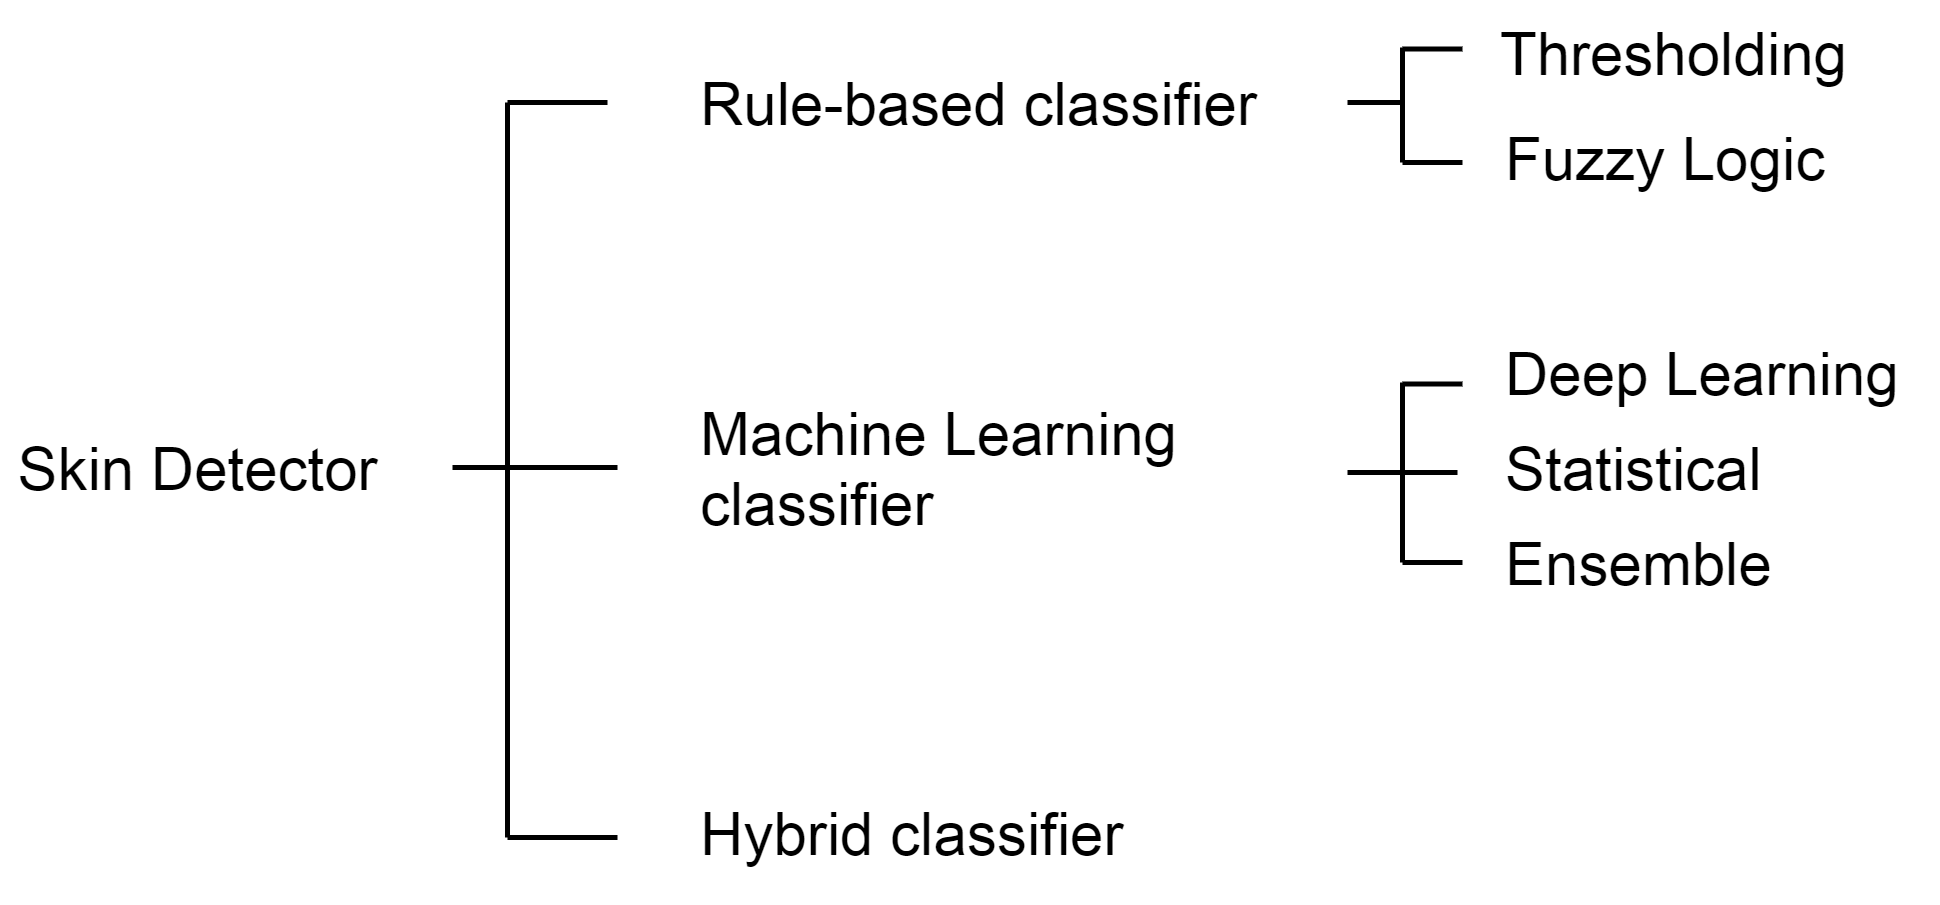
\includegraphics[width=0.9\linewidth]{images/introduction/taxonomy.png}
	\caption{Taxonomy of skin detectors.}
	\label{fig:taxonomy}
\end{figure}

\noindent{This section describes some common skin detection approaches. A chronological organization of the review with regards to the proposed taxonomy is reported in \autoref{tab:state-of-the-art}.}\\
\textbf{Jones and Rehg 2002}~\cite{jones2002statistical} is a machine learning statistical method based on the construction of a skin-color histogram model from an image database.
Then, a Bayesian classifier uses the model to make predictions on the desired images. The histogram model is built from an image database by analyzing the frequency that every pixel (R,G,B) combination has to be either skin or non-skin.
The Bayes rule utilizes a threshold to classify pixels based on their probability of being skin pixels.\\
\textbf{Kovac \textit{et al.} 2003}~\cite{kovac2003human} is a rule-based thresholding method that uses the union of a pair of rules to segment skin regions.
The first rule specializes in finding skin at uniform daylight illumination.
The second rule specializes in finding skin under flashlight or lateral daylight illumination.\\
\textbf{Chen and Wang 2007}~\cite{chen2007region} is a hybrid approach consisting of four main stages: image segmentation, key skin region extraction, similarity measurement, and skin region classification.
In the first stage, an unsupervised segmentation of color-texture regions in images is applied to segment the image into homogeneous regions.
In the second stage, a skin extractor is used for extracting the key skin regions. Firstly, the candidates of key skin regions are chosen by a rule-based skin classifier.
Then, the confidence values of the candidate regions are calculated as the proportion of the detected skin pixel count to the total pixel count of the region. The region with the largest confidence value will be the key skin region.
In the third stage, the similarity measure between the key skin region and all other regions is calculated to merge more possibly skin regions.
In the last stage, an algorithm is used to determine whether a region should be classified as a skin region or a non-skin region.
The algorithm calculates the pixels overlap ratio of the two 2D skin-color histograms representing a region and the key skin region, and then utilizes a threshold to classify the region.\\
\textbf{Khan \textit{et al.} 2010}~\cite{khan2010skin} is a machine learning ensemble approach that utilizes a random forest, an ensemble of tree predictors, to classify skin regions.
The input is presented to each of the trees in the forest.
Each tree gives an independent classification prediction and \q{votes} for that class.
The forest chooses the classification having the most votes. An image database is used to train the forest trees.\\
\textbf{Iraji and Yavari 2011}~\cite{iraji2011skin} is a rule-based fuzzy logic approach that defines a set of rules in the YCbCr color space to distinguish skin and non-skin pixels.
There may be pixels whose color acts both as skin color and as non-skin color.
Thanks to fuzzy logic with a Mamdani inference system (based on the implication rules), it is possible to get a unique membership value for each pixel, making the classification straightforward.\\
\textbf{Kawulok \textit{et al.} 2014}~\cite{Kawulok2014EURASIP} is a hybrid method that combines spatial analysis on top of a machine learning classifier.
First, the input image is converted into a skin probability map using a statistical histogram skin color model and a Bayesian classifier.
Then, the probability map is processed to find seed pixels.
The initial seed pixels are expanded using distance transform to include more skin pixels.
Subsequently, a local skin color model is trained from the obtained result and used to detect further skin pixels.
Finally, the distance transform is applied one more time.\\
\textbf{Brancati \textit{et al.} 2017}~\cite{brancati2017human} is a rule-based thresholding approach that works in the YCbCr color space.
Dynamic correlation rules are used to evaluate the combinations of chrominance values to identify the skin pixels in the YCb and YCr subspaces.
The correlation rules depend on the shape and size of dynamically generated skin color clusters computed in the YCb and YCr subspaces.\\
\textbf{He \textit{et al.} 2019}~\cite{he2019semi} is a deep learning method based on a dual-task CNN for joint detection of skin and body.
The dual-task network contains a shared encoder but two decoders for skin and body separately.
For each decoder, its output also serves as a guide for its counterpart, making both decoders mutually guided.\\
\textbf{Tarasiewicz \textit{et al.} 2020}~\cite{tarasiewicz2020skinny} proposed Skinny, a deep learning approach based on an encoder-decoder CNN architecture called U-Net.
Inception and dense block are inserted into a modified U-Net architecture to benefit from a wider spatial context.\\

\begin{table}[!htbp]
    \centering
    \resizebox{\textwidth}{!}{
    \begin{tabular}{lccc}
    \toprule
    \textbf{Name} & \textbf{Year} & \textbf{Category} & \textbf{Subcategory} \\
    \midrule
         Tarasiewicz \textit{et al.}~\cite{tarasiewicz2020skinny} & 2020 & Machine Learning & Deep Learning: CNN\\
         He \textit{et al.}~\cite{he2019semi} & 2019 & Machine Learning & Deep Learning: CNN\\ % Dual Decoder
         Brancati \textit{et al.}~\cite{brancati2017human} & 2017 & Rule-based & Thresholding\\
         Kawulok \textit{et al.}~\cite{Kawulok2014EURASIP} & 2014 & Hybrid & Machine Learning + Spatial Analysis\\ % Spatial Analysis
         Iraji and Yavari~\cite{iraji2011skin} & 2011 & Rule-based & Fuzzy Logic\\
         Khan \textit{et al.}~\cite{khan2010skin} & 2010 & Machine Learning & Ensemble: RandomForest\\
         Chen and Wang~\cite{chen2007region} & 2007 & Hybrid & Rule-based + Region-growing\\
         Kovac \textit{et al.}~\cite{kovac2003human} & 2003 & Rule-based & Thresholding\\
         Jones and Rehg~\cite{jones2002statistical} & 2002 & Machine Learning & Statistical: Bayes\\
    \bottomrule
    \end{tabular}}
  \caption{%
    Common approaches to Skin Detection, sorted by year in descending order.
  }
  \label{tab:state-of-the-art}
\end{table}

  %%%%%%%%%%%%%%%%%%%%%%%%%%%%%%%%%%%%%%%%%%%%%%%%%%%%%%%%%%%%%%%%%%%%%%%%
\chapter{Datasets}\label{chap:datasets}
%%%%%%%%%%%%%%%%%%%%%%%%%%%%%%%%%%%%%%%%%%%%%%%%%%%%%%%%%%%%%%%%%%%%%%%%


\noindent The importance of databases can be demonstrated by looking at the challenges in the field of Artificial Intelligence.
For years, the research on Artificial Intelligence has focused on the same concept: a better algorithm would make better decisions, regardless of the data.
However, even the best algorithm would not work well if the learned data didn't reflect the real world.\\
A good dataset is one that fits the desired purpose.
However, there are some general considerations that indicate good quality in a dataset.
Completeness, balanced classes, good organization, and quality labeling define a dataset of high quality.

In skin detection, a dataset usually consists of two types of pictures: the original images and the labeled images.
Labeled images are the ground truths and can either be binary masks or segmentation masks, where only the skin pixels are present.
Some datasets focus on the skin of a specific body part, such as the face or the abdomen.


%%%%%%%%%%%%%%%%%%%%%%%%%%%%%%%%%%%%%%%%%%%%%%%%%%%%%%%%%%%%%%%%%%%%%%%%
\section{Datasets Overview}
%%%%%%%%%%%%%%%%%%%%%%%%%%%%%%%%%%%%%%%%%%%%%%%%%%%%%%%%%%%%%%%%%%%%%%%%

A summary of common skin detection datasets is presented in \autoref{tab:dataset_table}, starting from the oldest to the newest. Only public datasets featuring images and including ground truths are considered.\\ 
\textbf{TDSD}~\cite{zhu2004adaptive} is the acronym of Test Database for Skin Detection, which is a database featuring 555 full-body skin images. Its ground truths are segmentation masks. It is also referred to as IBTD.\\
\textbf{ECU}~\cite{phung2005skin} is a dataset created at the Edith Cowan University and represents the largest analyzed dataset, consisting of 3998 pictures. It has been categorized as a full-body dataset, but most of its content is half-body shots. It can also be referred to as Face and Skin Detection Database (FSD).\\
\textbf{Schmugge}~\cite{schmugge2007objective} is a facial dataset that includes 845 images taken from different databases. It provides several labeled information about each image and ternary ground truths.\\
\textbf{Pratheepan}~\cite{tan2011fusion} is composed of 78 pictures randomly sampled from the web, precisely annotated\cite{osman2016improved}. It stores the pictures containing a single subject with simple backgrounds and images containing multiple subjects with complex backgrounds in different folders.\\
\textbf{VPU}~\cite{sanmiguel2013skin}, as for Video Processing \& Understanding Lab, consists of 285 images taken from five different public datasets for human activity recognition. The size of the pictures is constant between the images of the same origin. The dataset provides native train and test splits. It can also be referred to as VDM.\\
\textbf{SFA}~\cite{casati2013sfa} is the acronym of Skin of FERET and AR Database and consists of 1118 semi-passport pictures with a very plain background, and skin and non-skin samples (ignored in this work). Its ground truths are segmentation masks.\\
\textbf{HGR}~\cite{Kawulok2014EURASIP} is a Hand Gesture Recognition Database that organizes 1558 hand gesture images in three sub-datasets. Two sub-datasets include size-fixed very high-resolution images together with downscaled alternatives (used in this work).\\
\textbf{abd-skin}~\cite{topiwala2019adaptation} is a database composed of 1400 size-fixed abdominal pictures accurately selected to represent different ethnic groups and body mass indices. It has native test and train splits.\\

\begin{table}[h]
    \centering
    \resizebox{\textwidth}{!}{
    \begin{tabular}{lcccc}
    \toprule
    \textbf{Name} & \textbf{Year} & \textbf{No. of Images} & \textbf{Shot Type} & \textbf{Skin Tones\textsuperscript{1}} \\
    \midrule
         abd-skin~\cite{topiwala2019adaptation} & 2019 & 1400 & abdomen & african, indian, hispanic, caucasian, asian\\
         HGR~\cite{Kawulok2014EURASIP} & 2014 & 1558 & hand & -\\
         SFA~\cite{casati2013sfa} & 2013 & 1118 & face & asian, caucasian, negro\\
         VPU~\cite{sanmiguel2013skin} & 2013 & 285 & full body & -\\
         Pratheepan~\cite{tan2011fusion} & 2012 & 78 & full body & -\\
         Schmugge~\cite{schmugge2007objective} & 2007 & 845 & face & skintones labels: light, medium dark\\
         ECU~\cite{phung2005skin} & 2005 & 3998 & full body & whitish, brownish, yellowish, and darkish\\
         TDSD~\cite{zhu2004adaptive} & 2004 & 555 & full body & different ethnic groups\\
    \bottomrule
    \end{tabular}}
  \caption{%
    Common Datasets used in Skin Detection\\
    \textsuperscript{1}The \q{Skin tones} column reports either the ethnic diversity cited in the corresponding papers or the labels utilized for the skin tone values, in case they are present.
  }
  \label{tab:dataset_table}
\end{table}

\noindent A few notable public datasets are missing from the analysis for the following reasons.
\textbf{Compaq}~\cite{jones2002statistical} is the first large skin dataset consisting of 4675 labeled pictures. Ground truths are annotated with a semi-automatic process, hence the accuracy is not high~\cite{mahmoodi2015sdd}. Moreover, it is no longer available for public use~\cite{ruiz2006skindiff}. Despite the mentioned limitations, it is still used in the skin detection domain~\cite{brancati2017human, dourado2019domain}.\\
\textbf{LVS}~\cite{jones2002statistical} is an image database containing 2118 labeled frames. Labeled Video Sentences (LVS) contains original images and ground truths of skin and non-skin regions. The ground truth masks do not include ambiguous skin regions. The ground truths are quite imprecise because features like eyes and mouth are counted as skin pixels, as seen in \autoref{fig:lvs-gt}.\\
Some databases have been discarded because they do not use images: 
\textbf{Feeval}~\cite{stottinger2009skin} uses video sequences;  \textbf{UCI}~\cite{bhatt2009efficient} contains a list of skin and non-skin pixels in the BGR color space.

\begin{figure}[h]
     \centering
     \begin{subfigure}[b]{0.3\textwidth}
         \centering
         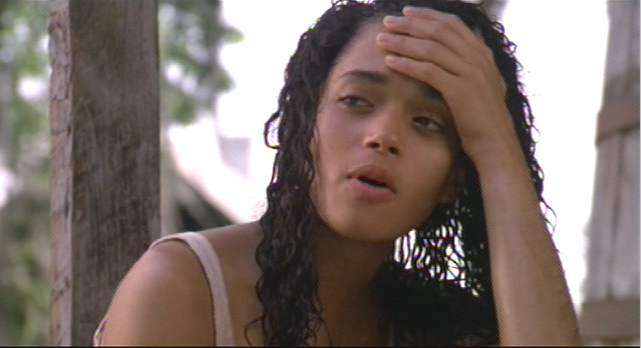
\includegraphics[width=\textwidth]{images/datasets/frame.25.png}
         \caption{}
         \label{fig:lvs-gt-x}
     \end{subfigure}
     \hfill
     \begin{subfigure}[b]{0.3\textwidth}
         \centering
         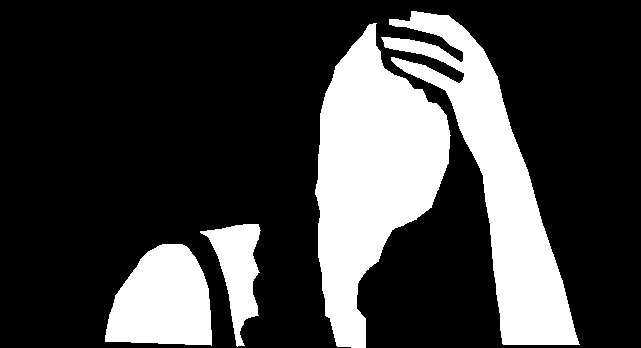
\includegraphics[width=\textwidth]{images/datasets/skin.25.png}
         \caption{}
         \label{fig:lvs-gt-skin}
     \end{subfigure}
    \hfill
     \begin{subfigure}[b]{0.3\textwidth}
         \centering
         
\includegraphics[width=\textwidth]{images/datasets/background.25.png}
         \caption{}
         \label{fig:lvs-gt-noskin}
     \end{subfigure}
        \caption{LVS~\cite{jones2002statistical} dataset example: (a) original image, (b) skin ground truth, (c) non-skin ground truth.
        Facial features like the eyes and mouth are treated as skin.}
        \label{fig:lvs-gt}
\end{figure}


%%%%%%%%%%%%%%%%%%%%%%%%%%%%%%%%%%%%%%%%%%%%%%%%%%%%%%%%%%%%%%%%%%%%%%%%
\section{Issues}
%%%%%%%%%%%%%%%%%%%%%%%%%%%%%%%%%%%%%%%%%%%%%%%%%%%%%%%%%%%%%%%%%%%%%%%%

Image databases are essential for developing skin detectors.
Over the years, new databases keep getting published, but there are still some limitations on their reliability.\\
The major limitations are described below, and some of them are illustrated in \autoref{fig:tdsd-gt}.

\begin{itemize}
    \item The number of pictures is sometimes not sufficiently high.
    \item The image quality is at times very low, and a sufficient intra-class variation is not present.
    \item The classes are often unbalanced, with one being much larger than the other, which may cause some metrics to give overoptimistic estimations~\cite{chicco2020advantages}.
    \item The ground truth labeling sometimes is performed using semi-automatic techniques, which give imprecise results~\cite{mahmoodi2015sdd}.
    Moreover, some skin regions are of dubious classification, especially the boundaries of the skin and around features such as eyes and mouth.
    \item Additional data is often cited in the original papers of the datasets, but not provided alongside it. Data about the lighting conditions, background complexity, number of subjects, indoor or outdoor scenery of an image may be extremely useful in some applications.
    \item Compression artifacts generated during the storage of ground truth masks represent another issue. The artifacts are inconvenient for either binary and segmentation masks and should be avoided by using lossless formats.
    \item Different skin tones are rarely evenly represented, and especially are not directly labeled.
    Furthermore, the categorization of skin tones does not follow a standard system and is questionable.
    \item Most image databases do not provide native training and testing splits, which confuses the evaluations in the literature.
\end{itemize}

\begin{figure}[!hbt]
     \centering
     \begin{subfigure}[b]{0.25\textwidth}
         \centering
         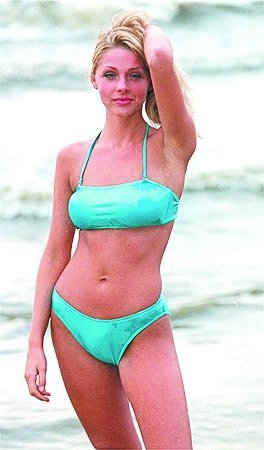
\includegraphics[width=\textwidth]{images/datasets/0487.jpg}
         \caption{}
         \label{fig:tdsd-gt-x}
     \end{subfigure}
     \hfill
     \begin{subfigure}[b]{0.25\textwidth}
         \centering
         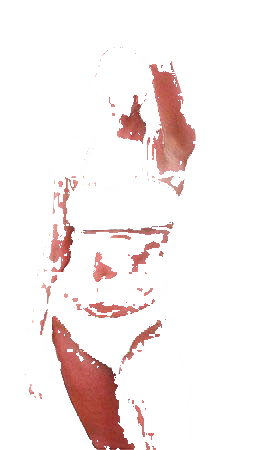
\includegraphics[width=\textwidth]{images/datasets/0487.png}
         \caption{}
         \label{fig:tdsd-gt-skin}
     \end{subfigure}
     \hfill
     \begin{subfigure}[b]{0.4\textwidth}
         \centering
         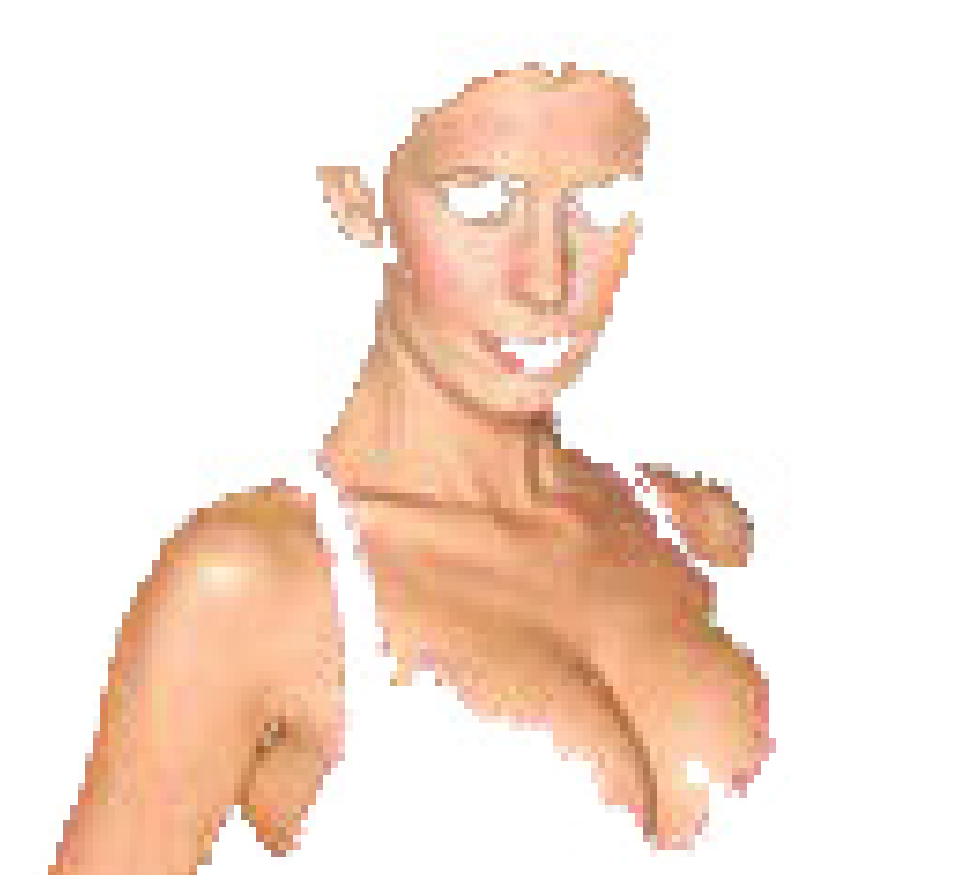
\includegraphics[width=\textwidth]{images/datasets/tdsd_artifacts.png}
         \caption{}
         \label{fig:tdsd-gt-noskin}
     \end{subfigure}
        \caption{TDSD~\cite{zhu2004adaptive} bad annotation examples: (a) original image No. 0487; (b) skin segmentation ground truth No. 0487; (c) compression artifacts.
        Test Database for Skin Detection (TDSD) contains both good and bad annotation examples. Ruiz-del-Solar and Verschae proposed three sub-dataset splits based on the annotation quality~\cite{ruiz2006skindiff}.
        Despite the issues, the dataset is important because, being born as a test dataset, it contains more uncorrelated images than those available in video datasets~\cite{bianco2015adaptive}.}
        \label{fig:tdsd-gt}
\end{figure}

%%%%%%%%%%%%%%%%%%%%%%%%%%%%%%%%%%%%%%%%%%%%%%%%%%%%%%%%%%%%%%%%%%%%%%%%
\section{Chosen Datasets}\label{sec:chosen-datasets}
%%%%%%%%%%%%%%%%%%%%%%%%%%%%%%%%%%%%%%%%%%%%%%%%%%%%%%%%%%%%%%%%%%%%%%%%

Accordingly to the issues previously mentioned, and considering the popularity, diversity, and size of the databases, the selected datasets for this work are ECU~\cite{phung2005skin}, HGR~\cite{Kawulok2014EURASIP} and Schmugge~\cite{schmugge2007objective}. A more detailed description of each one follows.

\noindent\textbf{ECU}~\cite{phung2005skin} is a dataset created at the Edith Cowan University that aims to support research on skin segmentation and face detection.
It contains 3998 pictures differing in terms of the depicted skin regions, skin tone types, lighting, and background, with both indoor and outdoor environments.
The authors did a rough categorization of the skin tones: 1665 images represent whitish and pinkish skin types; 1402 images represent yellowish and light brownish skin types; 965 images characterize reddish, darkish, and dark brownish skin types; the remaining ones generically represent other skin types.\\
\textbf{HGR}~\cite{Kawulok2014EURASIP} is a Hand Gesture Recognition Database of 1558 images. It organizes into three different sub-datasets: HGR1, HGR2A, and HGR2B.
HGR1 is a set of 899 pictures of various sizes and taken in uncontrolled light and background environments.
HGR2A contains 85 images of the same dimension taken in uniform lighting and both controlled and uncontrolled backgrounds.
HGR2B features 574 constant-sized pictures taken with a controlled background and in uniform lighting.
The skin tone diversity is very low as the images represent only a limited number of subjects.
Regarding the HGR2A and HGR2B sub-datasets, this work utilizes the downscaled versions of the pictures because high-resolution images would automatically be downscaled in approaches like neural networks.\\
\textbf{Schmugge}~\cite{schmugge2007objective} takes the name from its creator and consists of 845 images taken from different sources: the pictures representing skin pixels are collected from the AR face dataset~\cite{martinez1998ar}, the UOPB dataset~\cite{marszalec2000physics}, and the University of Chile dataset~\cite{ruiz2006skindiff}.
The first two include frontal facial images with varying illumination conditions and a very plain white background. Therefore, for these images, the non-skin pixels are not included.
The Chile dataset is composed of websites and digitized news clips and represents a variety of scenes, thus its non-skin pixels are included.
Other non-skin pixels are collected by randomly sampling the University of Washington content-based image retrieval database~\cite{berman1999flexible}.
Unlike other datasets, the ground truth follows a ternary representation: pixels are labeled as skin, non-skin, and \q{don't care}.
The \q{don’t care} label is assigned to pixels that are too ambiguous or tedious to label as either skin or non-skin.
This ternary division permits better management of pixels classification.
The dataset provides different files featuring additional data for each image, such as the skin tone, the light type, and the original database the picture is from. The ternary annotation system used in the dataset is shown in \autoref{fig:schmugge-ternary}.

\begin{figure}[hb]
    \centering
    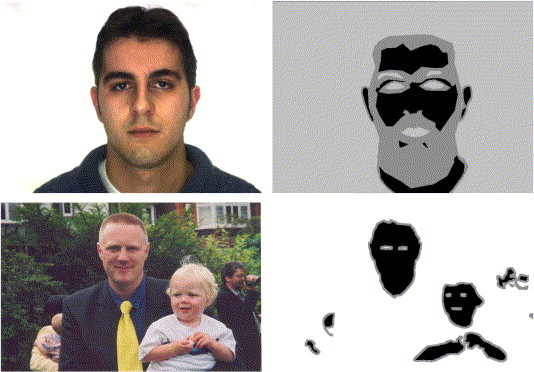
\includegraphics[width=0.7\linewidth]{images/datasets/schmugge_sample.jpg}
    \caption{Schmugge~\cite{schmugge2007objective} samples, RGB image on the left column and groundtruth on the right column. In annotations, skin pixels are black while non-skin pixels are white.
    Difficult and tedious regions to mark (\q{don’t care}) are colored in gray.
    The background in the top two images is marked in gray, indicating that those pixels did not participate in the evaluation. Adapted from Schmugge \textit{et al.} 2007~\cite{schmugge2007objective}}
    \label{fig:schmugge-ternary}
\end{figure}

  %%%%%%%%%%%%%%%%%%%%%%%%%%%%%%%%%%%%%%%%%%%%%%%%%%%%%%%%%%%%%%%%%%%%%%%%
\chapter{Investigated Methods}\label{chap:methods}
%%%%%%%%%%%%%%%%%%%%%%%%%%%%%%%%%%%%%%%%%%%%%%%%%%%%%%%%%%%%%%%%%%%%%%%%


\noindent As seen in \ref{sec:state-of-the-art}, there are several approaches to skin detection, and it can be confusing to make a choice.
All the different categories of methods are characterized by certain strength and weaknesses, therefore the choice to implement an approach should be made carefully.\\
\textbf{Rule-based} techniques represent a simple method to rapidly separate objects from their surroundings, don't require training, and generally are easy to implement.
However, color is the only feature they consider, and therefore the classification on backgrounds with skin-like colors, such as wood or clay, could be difficult.\\
\textbf{Machine learning} approaches are suitable when there is training data available.
There are several techniques with different features in this category.
Some uses only pixels color has the main drive for classification, while others manage to consider multiple features.\\
\textbf{Hybrid} methods are suitable when a single classification technique does not produce the desired results.

The chosen methods belong to the following categories: thresholding, traditional machine learning, deep learning.\\
Thresholding has been chosen because of the simplicity of the approach, which may demonstrate how powerful simple rules can be.\\
Machine learning and deep learning have been chosen for a comparison of their classification ability: it might be interesting to see how CNNs can learn about semantics from images~\cite{dharmaretnam2018emergence} and the comparison with respect to the traditional models.\\


\FloatBarrier
%%%%%%%%%%%%%%%%%%%%%%%%%%%%%%%%%%%%%%%%%%%%%%%%%%%%%%%%%%%%%%%%%%%%%%%%
\section{Thresholding}
%%%%%%%%%%%%%%%%%%%%%%%%%%%%%%%%%%%%%%%%%%%%%%%%%%%%%%%%%%%%%%%%%%%%%%%%

Thresholding methods are based on the idea that human skin can be grouped in clusters within a color space.
Therefore, the main process is to define the boundaries of the clusters.
Color images are segmented by designating separate thresholds for each color component, as seen in \autoref{fig:thresh-cube}.
The pixels falling within the range of these thresholds are classified as skin pixels.

There are static and dynamic thresholding methods.
\textbf{Static thresholding} consists of simple fixed rules to define the cluster boundaries.
In \textbf{Dynamic thresholding} the rules defining the boundaries depend on some variables.

\begin{figure}[h]
    \centering
    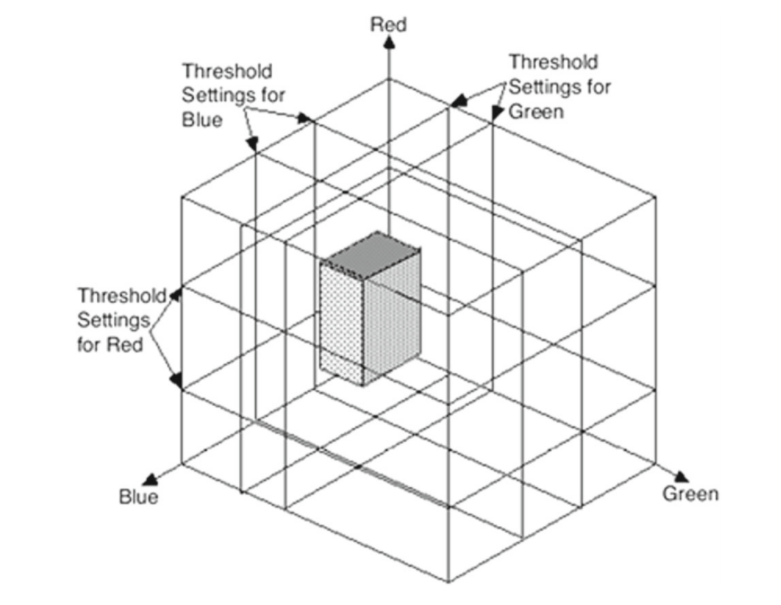
\includegraphics[width=0.7\linewidth]{images/approaches/thresholding/thresh_cube.png}
    \caption{Separate threshold settings for each color component.
    The shaded area is the Boolean AND of the three threshold settings. Adapted from John C. Russ 2007~\cite{zbMATH05833717}}
    \label{fig:thresh-cube}
\end{figure}

In literature, there isn't an agreement on the best color space to use. Nonetheless, to select the most suitable color space, its features should be taken into account.
For example, RGB describes a high correlation between color channels. An interesting technique to increase the detector accuracy is to combine channels of different color spaces~\cite{bin2007rgb}.
Several color spaces have been tested over the years: RGB~\cite{kovac2003human, cheddad2009skin, chen2012statistical}, RGB-H-CbCr~\cite{bin2007rgb}, HSV~\cite{garcia1999face, baskan2002projection, do2007skin}, YUV~\cite{yao2001face, vadakkepat2008multimodal}, YCbCr~\cite{garcia1999face, vadakkepat2008multimodal,  brancati2017human}.
Despite their simplicity, thresholding methods are relevant because of their low computational cost.
Their efficiency makes hardware implementations suitable, for example on Field Programmable Gate Array (FPGA)~\cite{chen2012statistical}.\\
An example of threshold rules in the RGB color space is presented below (taken from Kovac \textit{et al}. 2003~\cite{kovac2003human}):

\begin{minipage}{\linewidth}
\begin{verbatim}
    # The skin colour at uniform daylight illumination
    R > 95 AND G > 40 AND B > 20 AND
    max{R, G, B} - min{R, G, B} > 15 AND
    |R - G| > 15 AND R>G AND R>B
    
    OR
    
    # The skin colour under flashlight or (light) daylight
    # lateral illumination
    R > 220 AND G > 210 AND B > 170 AND
    |R - G| <= 15 AND R>B AND G>B
\end{verbatim}
\end{minipage}


\FloatBarrier
%%%%%%%%%%%%%%%%%%%%%%%%%%%%%%%%%%%%%%%%%%%%%%%%%%%%%%%%%%%%%%%%%%%%%%%%
\subsection{Implementation}\label{sec:impl-thresh}
%%%%%%%%%%%%%%%%%%%%%%%%%%%%%%%%%%%%%%%%%%%%%%%%%%%%%%%%%%%%%%%%%%%%%%%%

The chosen implementation\footnote{Source code available at \url{https://github.com/nadiabrancati/skin\_detection/}} is a dynamic thresholding approach~\cite{brancati2017human} published in 2017.
An overview of the algorithm is presented below:

\begin{enumerate}[Step 1:]
\item RGB to YCbCr conversion
\item Computation of $Cr_{max}$ and $Cb_{min}$
\item Pixel-wise computation of correlation rules parameters
\item Pixel-wise correlation rules check
\end{enumerate}

The method works in the YCbCr color space, so the first thing it does is the conversion of an RGB input image by using the ITU-R BT.601-5 conversion~\cite{bt2011studio}.
The skin pixels clusters assume a trapezoidal shape in the YCb and YCr color subspaces, as seen in \autoref{fig:trapeze-illuminations}.
Moreover, the shape and size of the trapezium vary according to many factors, such as the illumination conditions. 

In high illumination conditions, the base of the trapezium results larger.
Besides, the chrominance components of a skin pixel P with coordinates ($P_Y$, $P_{Cb}$, $P_{Cr}$) in the YCbCr space exhibit the following behavior: the further is the ($P_Y$, $P_{Cr}$) point from the longer base of the trapezium in the YCr subspace, the further is the ($P_Y$, $P_{Cb}$) point from the longer base of the trapezium in the YCb subspace, and vice versa.

\begin{figure}[h]
    \centering
    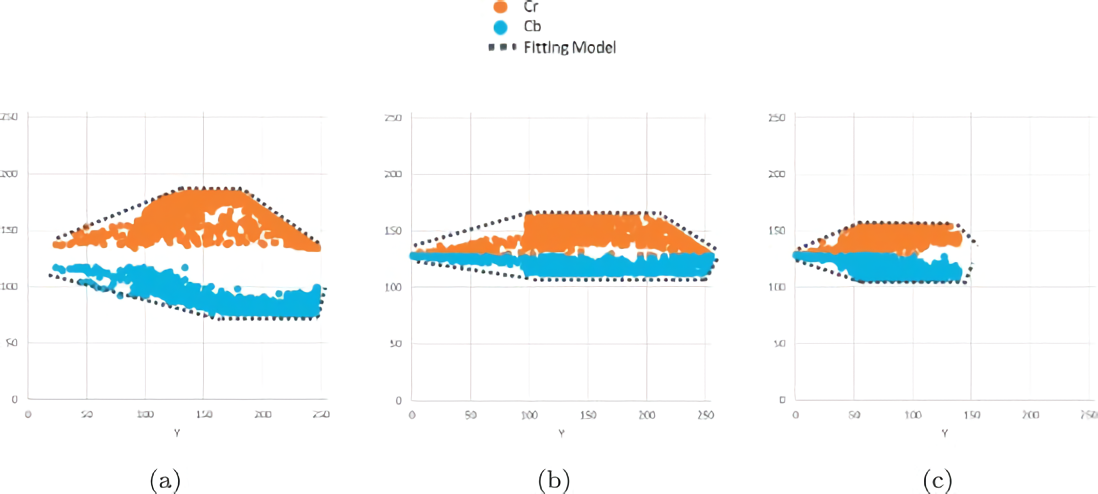
\includegraphics[width=0.9\linewidth]{images/approaches/thresholding/trapezia_illuminations.png}
    \caption{Fitting model for the YCb and YCr subspaces, in different conditions of illumination: (a) indoors with artificial light (b) outdoors with sunlight and (c) with low lighting.
    Adapted from Brancati \textit{et al.} 2017~\cite{brancati2017human}.}
    \label{fig:trapeze-illuminations}
\end{figure}

The aforementioned observations are the base of the method: it tries to define image-specific trapeziums in the YCb and YCr color subspaces and then verifies that the correlation rules between the two subspaces reflect the inversely proportional behavior of the chrominance components.

The first step is the computation of the height of the trapeziums in the YCb and YCr subspaces (the trapeziums are referred to as $T_{YCb}$ and $T_{YCr}$ in the following), which will be useful later on.
Referring to \autoref{fig:trapeze-other-sides} for a visual representation, it can be noticed that by varying the $Y$ value from its minimum value $0$, to its maximum value $255$, the coordinates of points belonging to the longer bases of $T_{YCr}$ and $T_{YCb}$ are given by ($Y$,$Cr_{min}$) and ($Y$,$Cb_{max}$) in the YCr and YCb subspaces.
The coordinates of points belonging to the remaining sides of the trapezium are given by [$Y$,$H_{Cr}(Y)$] and [$Y$, $H_{Cb}(Y)$] with:

\begin{equation}
\begin{aligned}
&H_{C r}(Y)=\left\{\begin{array}{ll}
C r_{\min }+h_{C r}\left(\frac{Y-Y_{\min }}{Y_{0}-Y_{\min }}\right) & Y \in\left[Y_{\min }, Y_{0}]\right. \\
C r_{\max } & Y \in\left[Y_{0}, Y_{1}\right] \\
C r_{\min }+h_{C r}\left(\frac{Y-Y_{\max }}{Y_{1}-Y_{\max }}\right) & \left.Y \in[ Y_{1}, Y_{\max }\right]
\end{array}\right. \\
&H_{C b}(Y)=\left\{\begin{array}{ll}
C b_{\min }+h_{C b}\left(\frac{Y-Y_{2}}{Y_{\min }-Y_{2}}\right) & Y \in\left[Y_{\min }, Y_{2}]\right. \\
C b_{\min } & Y \in\left[Y_{2}, Y_{3}\right] \\
C b_{\min }+h_{C b}\left(\frac{Y-Y_{3}}{Y_{\max }-Y_{3}}\right) & \left.Y \in[ Y_{3}, Y_{\max }\right]
\end{array}\right.
\end{aligned}
\end{equation}

where $h_{Cr} = Cr_{max} - Cr_{min}$ and $h_{Cb} = Cb_{max} - Cb_{min}$ represent the heights of $T_{YCr}$ and $T_{YCb}$, respectively.

\noindent The $Cr_{max}$ and $Cb_{min}$ values are computed by taking into account the histogram of the pixels with the following values: $Cr \in [Cr_{min}, 183]$ and $Cb \in [77,Cb_{max}]$, looking for the maximum of Cr and the minimum of Cb that are associated with at least 10\% of the pixels in the image.
The $Y_0$ and $Y_1$ values are respectively set as the 5th percentile and the 95th percentile of the luminance values associated with the pixels of the image with $Cr = Cr_{max}$.
The same procedure is followed to find the $Y_2$ and $Y_3$ values, considering the pixels with $Cb = Cb_{min}$. This process is illustrated in \autoref{fig:dyc-percentile}.

\begin{figure}[!htb]
	\centering
	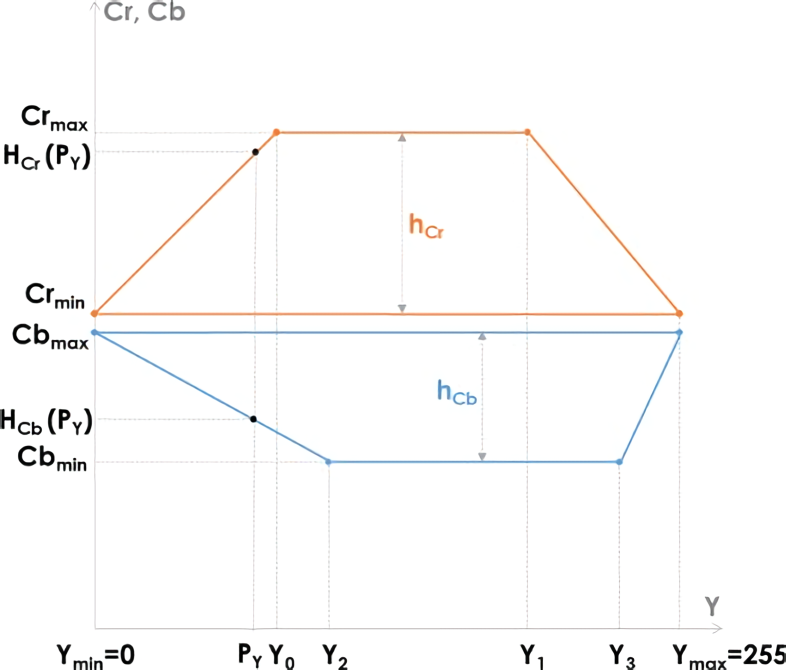
\includegraphics[width=0.6\linewidth]{images/approaches/thresholding/trapezia_other_sides.png}
	\caption{Graphical representation of $T_{YCr}$ and $T_{YCb}$. Adapted from Brancati \textit{et al.} 2017~\cite{brancati2017human}.}
	\label{fig:trapeze-other-sides}
\end{figure}

\begin{figure}[!htb]
	\centering
	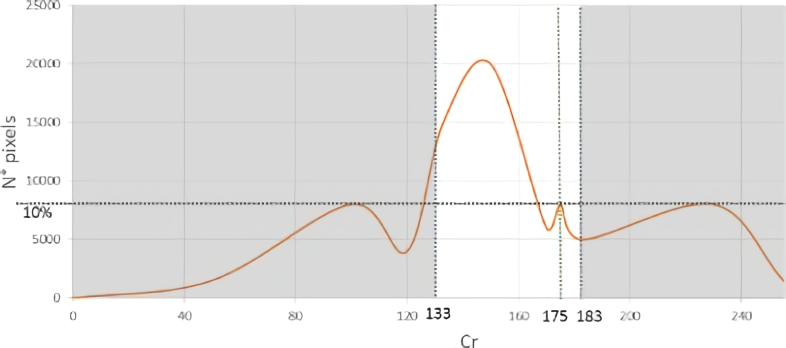
\includegraphics[width=0.9\linewidth]{images/approaches/thresholding/dyc_percentile.png}
	\caption{Computation of $Cr_{max}$ on the histogram of Cr values. Adapted from Brancati \textit{et al.} 2017~\cite{brancati2017human}.}
	\label{fig:dyc-percentile}
\end{figure}

The correlation rules between the chromatic components $P_{Cr}$ and $P_{Cb}$ of a pixel $P$ are defined by the computation of some parameters, as follows:

\begin{equation}
\begin{aligned}
&P_{C r}-P_{C b} \geq I_{P} \\
\end{aligned}
\end{equation}

\begin{equation}
\begin{aligned}
&\left|P_{C b}-P_{C b_{s}}\right| \leq J_{P}\\
\end{aligned}
\end{equation}

where $I_P$ is the minimum difference between the values $P_{Cr}$ and $P_{Cb}$, $P_{C b_{s}}$ is an estimated value of $P_{Cb}$, and $J_P$ is the maximum distance between the points $(P_Y, P_{Cb})$ and $(P_Y, P_{C b_{s}})$.

\noindent A pixel $P$ is classified as a skin pixel if both the conditions hold. The first rule indicates that the chrominance components should be sufficiently far from each other.
The second represents the range of values delimiting the $P_{C b_{s}}$ value, to which the $P_{Cb}$ should belong. \autoref{fig:trapeze-params} gives a visual representation of the operations to perform to compute the required parameters.

\begin{figure}[h]
	\centering
	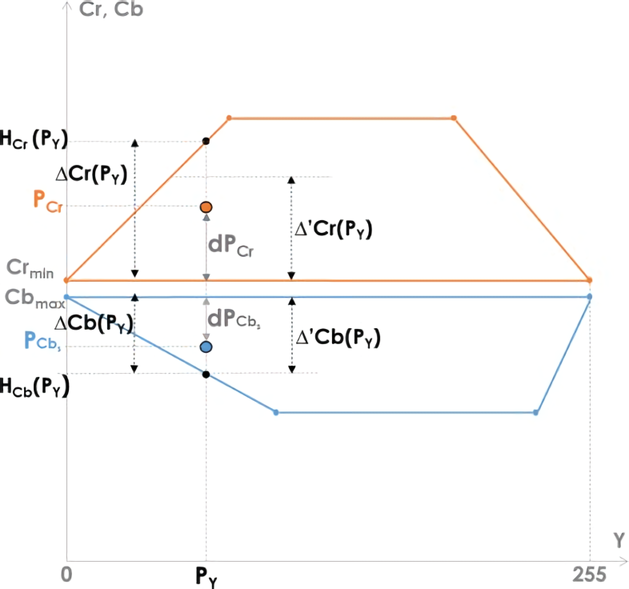
\includegraphics[width=0.6\linewidth]{images/approaches/thresholding/trapezia_params.png}
	\caption{Computation of the correlation rules parameters. Adapted from Brancati \textit{et al.} 2017~\cite{brancati2017human}.}
	\label{fig:trapeze-params}
\end{figure}

\begin{equation}
\begin{aligned}
P_{C b_{s}} = Cb_{max} - dP_{C b_{s}}\\
P_{Cr} = Cr_{min} + dP_{Cr}
\end{aligned}
\end{equation}

with $dP_{C b_{s}}$ and $dP_{Cr}$ as the distances respectively between the points $(P_Y, P_{C b_{s}})$ and $(P_Y, P_{Cr})$, and the longer bases of the trapezium in the corresponding subspaces.
It is possible to compute $dP_{C b_{s}}$ with respect to $dP_{Cr}$ on the basis of the inversely proportional behavior of the chrominance components observed within the trapezium:

\begin{equation}
\begin{aligned}
dP_{C b_{s}} = \alpha \cdot dP_{Cr}
\end{aligned}
\end{equation}

where $\alpha$ takes into account the different shapes of the trapezium, being computed as the ratio between the normalized heights of the two trapeziums in correspondence with the current luminance value $P_Y$ as follows:

\begin{equation}
\begin{aligned}
\Delta_{Cr}(P_Y) = H_{Cr}(P_Y) - Cr_{min}\\
\Delta_{Cb}(P_Y) = Cb_{max} - H_{Cb}(P_Y)
\end{aligned}
\end{equation}

where $\Delta_{Cr}(P_Y)$ and $\Delta_{Cb}(P_Y)$ represent the distances between the points $(P_Y, H_{Cr}(P_Y))$ and $(P_Y, H_{Cb}(P_Y))$ and the longer base of their respective trapezium.

\noindent Now, the values of $\Delta_{Cr}(P_Y)$ and of $\Delta_{Cb}(P_Y)$ are normalized with respect to the difference in the size of the trapeziums:

\begin{equation}
\begin{aligned}
&\Delta_{C r}^{\prime}\left(P_{Y}\right)=\left\{\begin{array}{ll}
\Delta_{C r}\left(P_{Y}\right) \cdot \frac{A_{T_{YCb}}}{A_{T_{YCr}}} & \text { if } A_{T_{YCr}} \geq A_{T_{YCb}} \\
\Delta_{C r}\left(P_{Y}\right) & \text { otherwise }
\end{array}\right. \\ \\
&\Delta_{C b}^{\prime}\left(P_{Y}\right)=\left\{\begin{array}{ll}
\Delta_{C b}\left(P_{Y}\right) & \text { if } A_{T_{YCr}} \geq A_{T_{YCb}} \\
\Delta_{C b}\left(P_{Y}\right) \cdot \frac{A_{T_{YCr}}}{A_{T_{YCb}}} & \text { otherwise }
\end{array}\right.
\end{aligned}
\end{equation}

where $A_{T_{YCr}}$ and $A_{T_{YCb}}$ are the areas of the trapeziums $T_{YCr}$ and $T_{YCb}$, respectively.
Then, the value $\alpha$ is given by:

\begin{equation}
\begin{aligned}
\alpha=\frac{\Delta_{C b}^{\prime}\left(P_{Y}\right)}{\Delta_{C r}^{\prime}\left(P_{Y}\right)}\\
\end{aligned}
\end{equation}

\noindent Finally, the remaining parameters $I_P$ and $J_P$ are given by:

\begin{equation}
\begin{aligned}
I_{P}=s f \cdot\left[\left(\Delta_{C r}^{\prime}(Y)-d P_{C r}\right)+\left(\Delta_{C b}^{\prime}(Y)-d P_{C b_{s}}\right)\right]
\\ \\
J_{P}=d P_{C b_{s}} \cdot \frac{d P_{C b_{s}}+d P_{C r}}{\Delta_{C b}^{\prime}(Y)+\Delta_{C r}^{\prime}(Y)}
\\ \\
s f=\frac{\min \left(\left(Y_{1}-Y_{0}\right),\left(Y_{3}-Y_{2}\right)\right)}{\max \left(\left(Y_{1}-Y_{0}\right),\left(Y_{3}-Y_{2}\right)\right)}
\end{aligned}
\end{equation}


\FloatBarrier
%%%%%%%%%%%%%%%%%%%%%%%%%%%%%%%%%%%%%%%%%%%%%%%%%%%%%%%%%%%%%%%%%%%%%%%%
\section{Statistical}
%%%%%%%%%%%%%%%%%%%%%%%%%%%%%%%%%%%%%%%%%%%%%%%%%%%%%%%%%%%%%%%%%%%%%%%%

Large amount of data can support simple and computationally efficient learning algorithms~\cite{jones2002statistical}.
Statistical methods aim at creating a model to understand how the data are related in order to make predictions (an example can be seen in \autoref{fig:statistical-model-example}).
When performing classification, these models not only allow to predict the class label, but also to obtain a probability of the respective label.
This probability gives the confidence on the prediction.

Given a probability, different rules can be used to perform the classifications, with one of the most common being the Bayes rule.
In binary classification problems, a single threshold is involved to choose at which probability one class should be classified over another.
The thresholding rule is not unique, multiple rules have been used in the literature~\cite{jones2002statistical, phung2001universal}.

% IN SKIN DETECTION
In skin detection, one of the most popular work of statistical modeling has been published in 2002~\cite{jones2002statistical}: a Bayesian classifier has been used to perform classifications starting from the probabilities given by statistical models.
In the same work, skin and non-skin gaussian mixture models using a parallel implementation of the standard EM algorithm~\cite{redner1984mixture} and $16$ gaussians in each model have been trained.
A comparison with histogram models of size $32$ is presented.
The results describe slightly better performance in the case of the histogram models, which also took only a matter of minutes to train, as opposed to about $24$ hours required by the gaussian mixture models.
A mixture model is also slower to use during classification since all the gaussians must be evaluated in computing the probability of a single color value.
Contrarily, a histogram model translates to a fast classifier since only two table lookups are required to compute the probability of skin.
However, from a storage point of view, the gaussian mixture models are much more compact: $896$ bytes in contrast to $262$ Kbytes of the histogram models.\\
Gomez \textit{et al.} 2002~\cite{gomez2002selecting} presented a work in which two 3-dimensional histogram models are constructed to represent the skin and non-skin classes, and the probability is computed with a rule different than the Bayes theorem.

\begin{figure}[h]
    \centering
    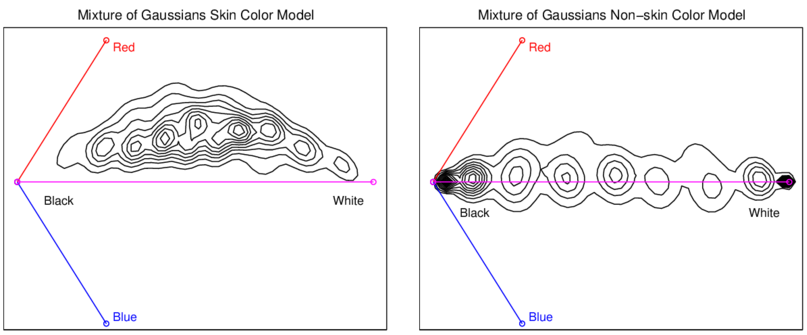
\includegraphics[width=0.9\linewidth]{images/approaches/statistical/statistical_model.png}
    \caption{Mixture of gaussians are an example of statistical models.
    Adapted from Jones and Rehg 2002~\cite{jones2002statistical}}
    \label{fig:statistical-model-example}
\end{figure}


\FloatBarrier
%%%%%%%%%%%%%%%%%%%%%%%%%%%%%%%%%%%%%%%%%%%%%%%%%%%%%%%%%%%%%%%%%%%%%%%%
\subsection{Implementation}\label{sec:impl-bayes}
%%%%%%%%%%%%%%%%%%%%%%%%%%%%%%%%%%%%%%%%%%%%%%%%%%%%%%%%%%%%%%%%%%%%%%%%

%% SPIEGO MODELLO SCELTO
The chosen implementation\footnote{Source code available at \url{https://github.com/Chinmoy007/Skin-detection}}\ uses three-dimensional histograms to model the data and probability calculus to perform the classification~\cite{acharjee2018skin}.
The training data is used to construct two histogram models representing the probabilities of skin and non-skin classes, with RGB as the color space and a histogram size of $256$ bins per color component.
The models are saved as a lookup table.
The thresholding value utilized to label skin pixels is $0.555555$.\\
An overview of the algorithm is presented below:
\vspace{5mm}

\begin{minipage}{\linewidth}%
\noindent Training:
    \begin{enumerate}[Step 1:]
    \item Initialize two 3-dimensional data structures
    \item Pick an image and the corresponding mask from the training dataset
    \item Loop every (R,G,B) pixel of the image
    \item Pick the corresponding pixel from the mask: if it is a skin pixel, increase the value at position [R, G, B] of the data structure representing skin, otherwise increase the value in the other structure
    \item Return to the first step until the training images have all been processed 
    \end{enumerate}
    
    \vspace{3mm}
    \noindent Predicting:
    \begin{enumerate}[Step 1:]
    \item Loop every (R,G,B) pixel from input image
    \item Calculate the probability of that (R,G,B) color combination of being skin
    \item If skin probability > $\Theta$, the pixel is classified as skin
    \end{enumerate}
\end{minipage}

\vspace{7mm}
\noindent The key step in skin pixel classification is the computation of $P (skin \mid rgb)$, which is the probability of a given $rgb$ pixel to belong to the skin class, and it is given by the following rule:

\begin{equation}
    P(skin \mid rgb) = \frac{s[rgb]}{s[rgb] + n[rgb]}
\end{equation}

where $s[rgb]$ is the pixel count contained in bin $rgb$ of the skin histogram and $n[rgb]$ is the equivalent count from the non-skin histogram.\\
% threshold
A particular RGB value is labeled skin if:

\begin{equation}
\label{eqn:bayes-thresh}
P(s k i n \mid r g b) \geq \Theta
\end{equation}

where  $0 \leq \Theta \leq 1 $ is a threshold value that can be adjusted to trade-off between true positives and false positives.

\noindent It is important to note that using color spaces other than RGB (such as YCBCr or HSV) will not improve the performance of the skin detector~\cite{jones2002statistical}.
The Detector performance depends entirely on the amount of overlap between the skin and non-skin samples. Colors that occur in both classes with comparable frequencies cannot be classified reliably.


%% HISTOGRAM MODEL DESCRIPTION - SPIEGO DETTAGLIATO
There are different ways to build the skin and non-skin color models.
One of the most common is to utilize \textbf{histogram models}: the skin and non-skin pixels contained in the training set images are placed into the skin and non-skin histograms, respectively.\\
Before constructing an histogram model, two requirements are needed: a color space and the size of the histogram, which is measured by the number of bins per color channel.
The fact that the performance of the classifier is independent of the color space, and RGB being the most common and natural color space used in image representation, makes RGB the favorite choice.
Color images usually store $24$ bits for each pixel, as there are three color components represented by $8$ bits each. Each color component is thereby able to represent $2^8=256$ levels of intensity.

\begin{figure}[h]
     \centering
     \begin{subfigure}[b]{0.45\textwidth}
         \centering
         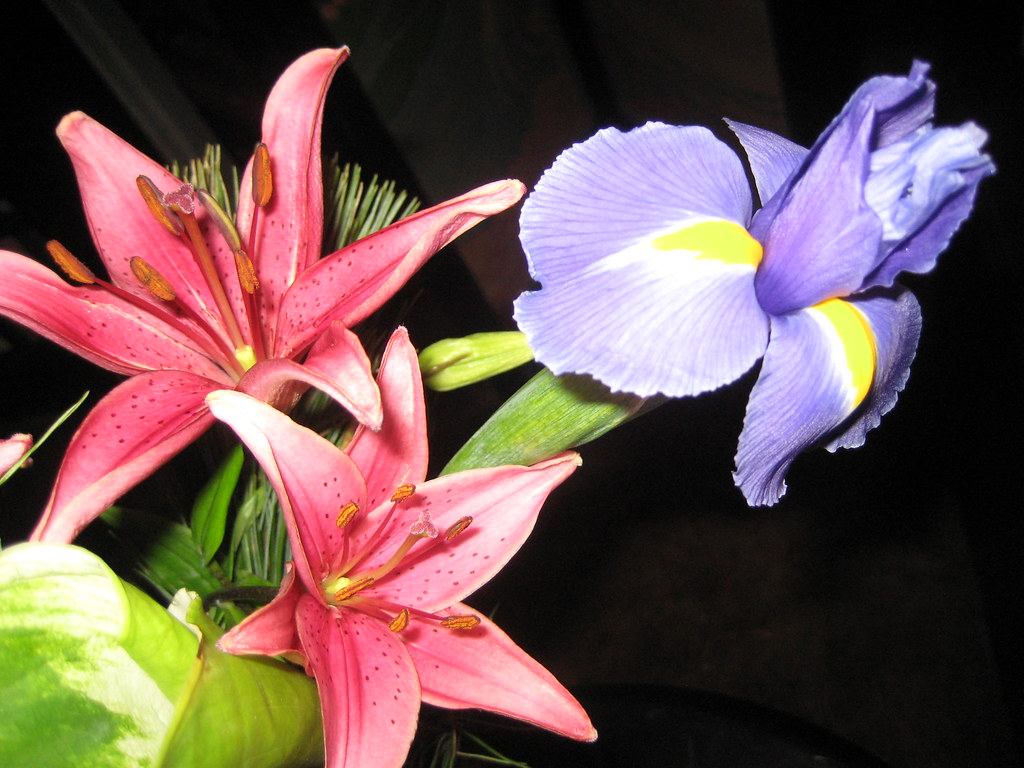
\includegraphics[width=\textwidth]{images/approaches/statistical/3d-hist-orig.jpg}
         \caption{}
         \label{fig:3d-hist-orig}
     \end{subfigure}
     \hfill
     \begin{subfigure}[b]{0.45\textwidth}
         \centering
         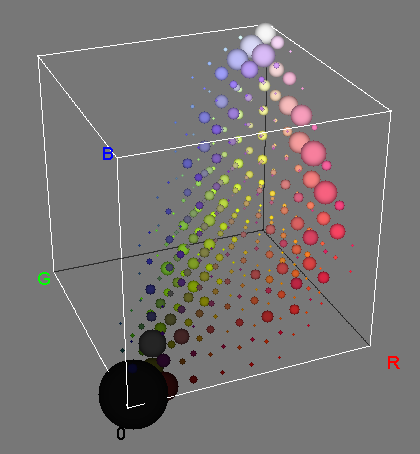
\includegraphics[width=\textwidth]{images/approaches/statistical/3d-hist-plug.png}
         \caption{}
         \label{fig:3d-hist-plug}
     \end{subfigure}
        \caption[footnote-3d]{3D histogram representation: (a) original photo by Jose and Roxanne licensed under CC BY 2.0; (b) visualization made utilizing the \q{3D Color Inspector} plugin of ImageJ.\footnotemark}
        \label{fig:3d-hist}
\end{figure}
\footnotetext{Plugin available at \url{https://imagej.nih.gov/ij/plugins/color-inspector.html}} % Anywhere on the same page where the float appears - TODO

When building the histogram, the number of bins is important. Too few bins could result in poor accuracy, while too many bins could lead to over-fitting~\cite{jones2002statistical}.
Reducing the number of bins helps to \q{generalise} and compact the histogram~\cite{gomez2002selecting}.
By using fewer bins, a set of points of similar color is represented by a single color (this technique is called color quantization. An example of a 3D histogram using the technique is depicted in \autoref{fig:3d-hist}).
By using a $24$-bit pixel representation, the histogram model would have a size of $256$ bins per color channel, which correspond to more than 16 million ($256^3$) bins, each mapped to a specific (R,G,B) color triple.
Jones and Rehg (2002)~\cite{jones2002statistical} found the best histogram size in their experiments to be $32$.
They also reported that, with a histogram size of $256$, $77\%$ of the possible $24$-bit RGB colors are never encountered, and thus the histogram is mostly empty.\\
Using a histogram size of $256$ in the RGB color space means that each of the three histogram dimensions is divided into $256$ bins. And each bin stores an integer counting the number of times that color value occurred in the entire database of images.


\FloatBarrier
%%%%%%%%%%%%%%%%%%%%%%%%%%%%%%%%%%%%%%%%%%%%%%%%%%%%%%%%%%%%%%%%%%%%%%%%
\section{Convolutional Neural Networks}
%%%%%%%%%%%%%%%%%%%%%%%%%%%%%%%%%%%%%%%%%%%%%%%%%%%%%%%%%%%%%%%%%%%%%%%%

Convolutional Neural Networks (CNNs) are a type of Neural Network commonly applied to analyze visual scenes. Their structure is inspired by the human brain, mimicking the way that biological neurons signal to one another.


\FloatBarrier
%%%%%%%%%%%%%%%%%%%%%%%%%%%%%%%%%%%%%%%%%%%%%%%%%%%%%%%%%%%%%%%%%%%%%%%%
\subsection{Neural Networks}
%%%%%%%%%%%%%%%%%%%%%%%%%%%%%%%%%%%%%%%%%%%%%%%%%%%%%%%%%%%%%%%%%%%%%%%%

A \textbf{biological neuron} has specialized protrusions called dendrites and axons.
Dendrites bring information to the cell body, and axons take information away from the cell body.
Information flows from one neuron to another across a small gap between them named synapse.
The dendrites carry the signal to the cell body where they all get summed; if the final sum is above a certain threshold, the neuron can fire, sending a spike along its axon.

\begin{figure}[h]
	\centering
	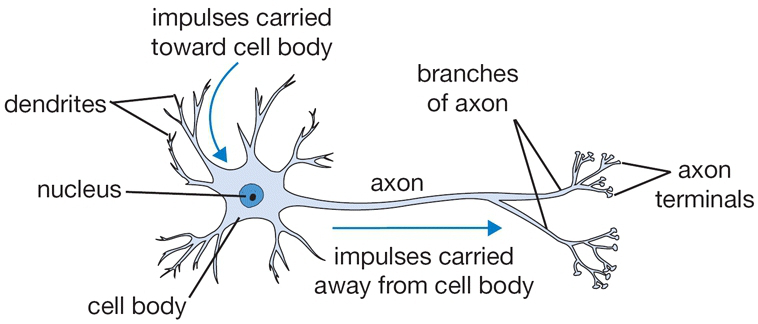
\includegraphics[width=0.7\linewidth]{images/approaches/deep_learning/neuron_b.png}
	\caption[footnote-3d]{Biological neuron.\footnotemark}
	\label{fig:neuron-bio}
\end{figure}
\footnotetext{The figure is adapted from \url{https://cs231n.github.io/neural-networks-1/}}

In the \textbf{computational model of a neuron}, also named Perceptron, the signals that travel along the axons $x_i$ interact multiplicatively $(w_ix_i)$ with the dendrites of the other neuron based on the synaptic strength $w_i$ at that synapse.
The dendrites bring the signals to the cell body, where they all get summed. The idea is that the synaptic strengths (the weights $w$) are learnable and control the strength of influence of one neuron on another. 
The neuron then performs a transformation to the input through the activation function $f(x)$ and generates the output $y$.
The activation function is typically a non-linear transformation that is applied to the input data.
The bias value $b$ allows the activation function to be shifted to the left or right, to better fit the data.
The weights and biases represent the parameters of the network.

\begin{figure}[htbp]
  \centering
  \includesvg[width=0.7\linewidth]{images/approaches/deep_learning/neuron_c.svg}
  \caption{Neuron computational model.}
  \label{fig:neuron-comp}
\end{figure}

A \textbf{Neural Network} is a group of multiple neurons connected together, as shown in \autoref{fig:forward-prop}.
Neurons are typically organized into different layers.
Neurons of one layer connect only to neurons of the immediately preceding and immediately following layers, therefore the output of a layer becomes the input of the next layer.
The first layer is the input layer, where each neuron represents a feature in the dataset, the last layer is the output layer, and all the other layers are the hidden layers.
Although a single output is depicted in the figure, the output layer can have different sizes. It can vary from one output for a single class classification to thousands of pixels of an image classification map.

\begin{figure}[h]
	\centering
	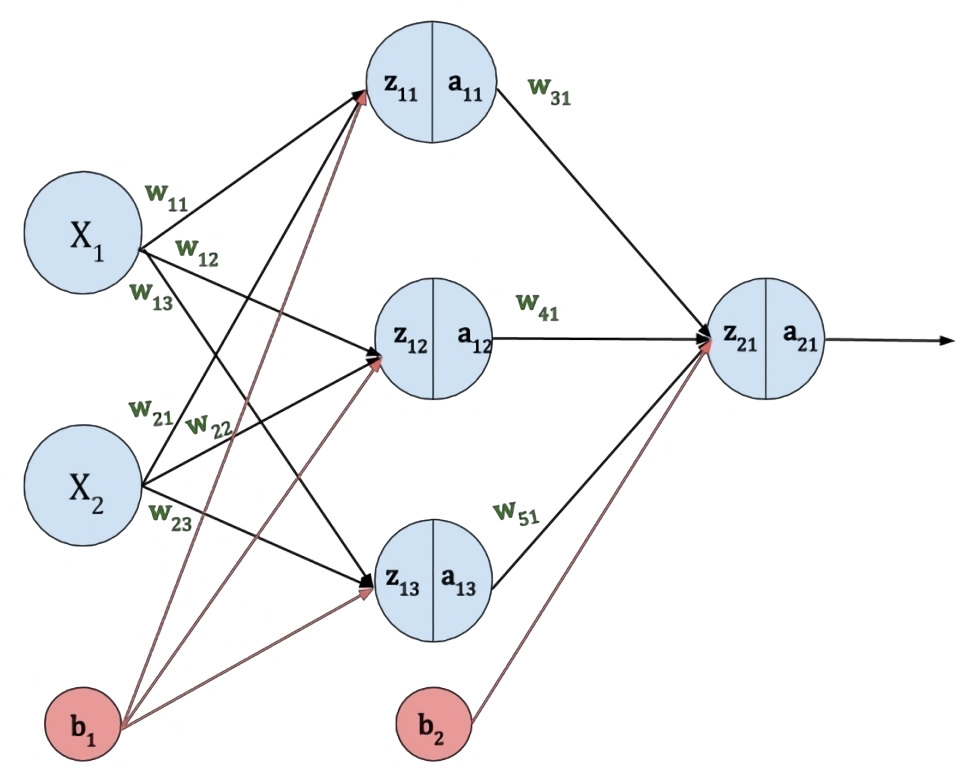
\includegraphics[width=0.7\linewidth]{images/approaches/deep_learning/forwardpass.jpg}
	\caption[footnote-3d]{A two-layer Neural Network architecture. Conventionally, the input layer is not counted for defining the number of layers of a Neural Network.
	There are two input features: $x_1$ and $x_2$, a hidden layer with three neurons, and an output layer with one neuron.
	Each neuron has assigned the weight parameter $W_{ij}$. The $b_1$ and $b_2$ are the bias parameters for the input layer and hidden layer, respectively.}
	\label{fig:forward-prop}
\end{figure}

\noindent Once the dataset and problem are defined, the main steps to train a Neural Network are the following:
\begin{enumerate}[Step 1:]
\item Construct the network architecture and initialize with random weights
\item Do a forward pass (Forward propagation)
\item Calculate the total error, which needs to be minimized
\item Back propagate the error and Update weights
\item Repeat the steps(2-4) for No. of epochs/until error is minimum.
\end{enumerate}

\noindent In \textbf{forward propagation}, the input data is fed to the network in the forward direction: each hidden layer gets the data, perform calculation and pass the result to the next layer.
Finally, the output layer calculates the output of the model.\\
The forward propagation for the network in \autoref{fig:forward-prop} is described below.
The input is represented by $X$, which can be imagined as a matrix of 2 rows and 1 column.
The next layer is represented by $z_{11}$, $z_{12}$, $z_{13}$, which are the values of the intermediate neurons calculated from the weight, bias, and neuron values of the previous layer.
This layer can be imagined as a matrix of 3 rows and 1 column.
In this case, there are two input nodes and three output nodes that the parameters must fit. $W_{\text {pln, nln }}^{\text {(layer) }}$ is the parameter to be optimized, in which $pln$ and $nln$ represent the previous layer input neuron and the next layer output neuron, respectively.
The bias parameter for the input layer is represented by $b_1$.

\begin{equation}
\begin{aligned}
{\left[\begin{array}{l}
z_{11} \\
z_{12} \\
z_{13}
\end{array}\right]=\left[\begin{array}{ll}
w_{11} & w_{21} \\
w_{12} & w_{22} \\
w_{13} & w_{23}
\end{array}\right]\left[\begin{array}{l}
x 1 \\
x 2
\end{array}\right]+\left[\begin{array}{l}
b_{1} \\
b_{1} \\
b_{1}
\end{array}\right]} \\
Z^{[1]}=W^{[1]} X+b^{[1]}
\end{aligned}
\end{equation}

\noindent An activation function $\sigma(Z)$ will be applied to the intermediate neuron values to learn the non-linear patterns between inputs and target output variables.
The $a_{11}$, $a_{12}$, and $a_{13}$ values are the output of the activation function that is applied to $z_{11}$, $z_{12}$ and $z_{13}$, respectively.

\begin{equation}
\begin{aligned}
\left[\begin{array}{l}
a_{11} \\
a_{12} \\
a_{13}
\end{array}\right] &=\sigma\left[\begin{array}{l}
z_{11} \\
z_{12} \\
z_{13}
\end{array}\right] \\
A^{[1]} &=\sigma\left(Z^{[1]}\right)
\end{aligned}
\end{equation}

\noindent At the next step, $A^{[1]}$ becomes the input layer and $z_{21}$ becomes the output layer.
There are three input nodes and an output node that the parameters must fit, so $W^{[2]}$ is a matrix with one row and three columns.
The bias parameter for the hidden layer is represented by $b_2$.

\begin{equation}
\begin{gathered}
{\left[z_{21}\right]=\left[\begin{array}{lll}
w_{31} & w_{41} & w_{51}
\end{array}\right]\left[\begin{array}{l}
a 11 \\
a 12 \\
a 13
\end{array}\right]+\left[b_{2}\right]} \\
Z^{[2]}=W^{[2]} A^{[1]}+b^{[2]}
\end{gathered}
\end{equation}

\noindent The activation function $\sigma(Z)$ is applied to the obtained values, and the algorithmic step represented by this layer finishes.

\begin{equation}
\begin{aligned}
&{\left[a_{21}\right]=\sigma\left[z_{21}\right]} \\
&A^{[2]}=\sigma\left(Z^{[2]}\right)
\end{aligned}
\end{equation}

\noindent The output of the neural network is calculated, hence the forward propagation algorithm ends.

\textbf{Activation functions} are an important part of Neural Networks.
Without them, the networks are just the weighted sum of their inputs plus a bias term, unable to learn any complex and nonlinear function.
Activation functions are means to introduce non-linearity to the model.
There are different classes of activation functions available, with common ones being the Sigmoid, the ReLU, the Tanh, and the Linear activation functions.
The mentioned activation functions are illustrated in \autoref{fig:activation-functions}.

\begin{figure}[h]
	\centering
	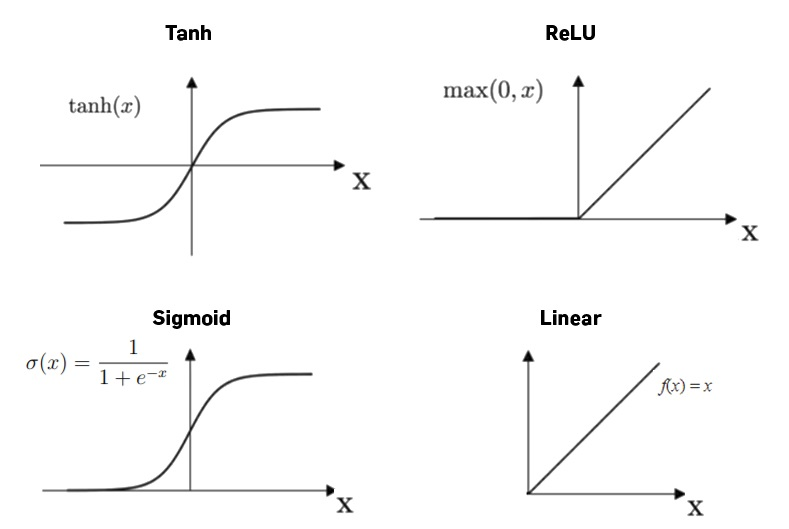
\includegraphics[width=0.9\linewidth]{images/approaches/deep_learning/activation_functions_f.jpg}
	\caption{Common activation functions. The Tanh function forces the values to be between $-1$ and $1$. The Sigmoid function forces the values to be between $0$ and $1$. The ReLU function cuts values below zero. The Linear activation function returns the input.}
	\label{fig:activation-functions}
\end{figure}

The next step in a Neural Network is to \textbf{compute the loss (error)}. Once the output of the network is obtained, it is compared to the desired output value (the so-called ground truth), and a loss function computes the error signal, which measures how well the network predicts outputs.\\
A popular loss function is the Cross-Entropy Loss, defined as follows:

\begin{equation}
\begin{aligned}
&J=-\frac{1}{m} \sum_{i=1}^{m} L\left(a^{[2](i)}, y^{(i)}\right) \\
&L\left(a^{[2]}, y\right)=-y \log a^{[2]}-(1-y) \log \left(1-a^{[2]}\right)
\end{aligned}
\end{equation}

where L is the loss function and J is the cost function: the average loss over the entire training dataset.

\noindent The goal is to then find a set of weights and biases that minimizes the error.
However, it is impossible to compute the error signal for internal neurons directly because the output values of these neurons are unknown.
The idea is to propagate the error signal back to all neurons by computing the gradient of the loss function with respect to each weight.
The derivative of the loss function on each parameter gives information about how changing the parameter impacts the function value.
The algorithm that computes the gradient is called \textbf{backpropagation}.

\begin{figure}[h]
	\centering
	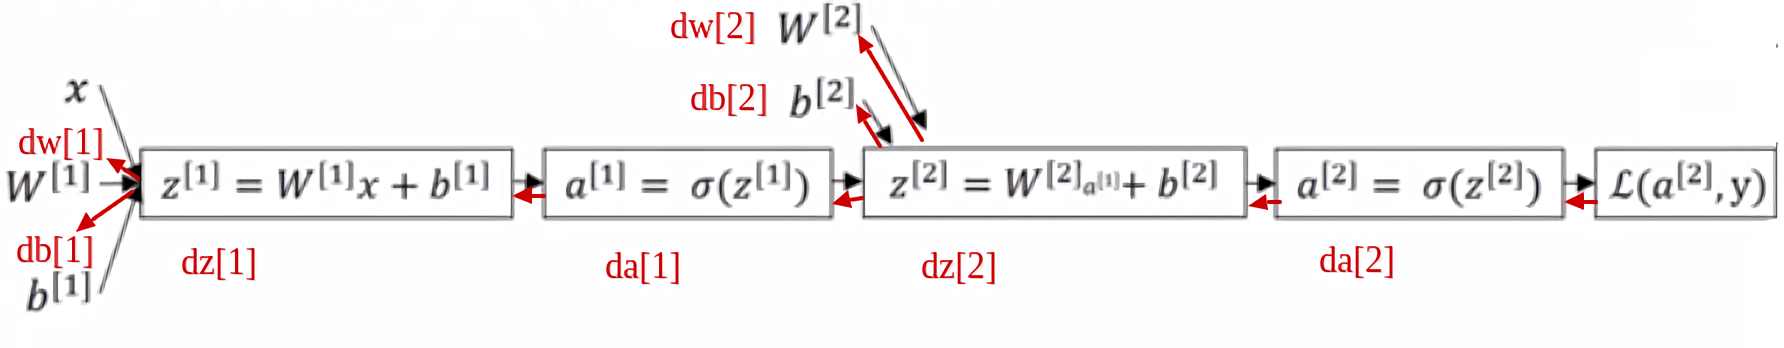
\includegraphics[width=0.9\linewidth]{images/approaches/deep_learning/backprop_nn.png}
	\caption[footnote-3d]{The red line represents the back-propagation process. The $da[2]$, $dz[2]$, $dw[2]$, $db[2]$, $da[1]$, $dz[1]$, $dw[1]$ and $db[1]$ are the partial derivative of the loss function with respect to $a[2]$, $z[2]$, $w[2]$, $b[2]$, $a[1]$, $z[1]$, $w[1]$ and $b[1]$ respectively.}
	\label{fig:backprop}
\end{figure}

While performing the derivative calculation, it is also necessary to calculate the derivative of the activation function. Below is presented the derivative of the Sigmoid Activation function:

\begin{equation}
\begin{aligned}
\sigma(x) &=\frac{1}{1+e^{-x}}=\left(1+e^{-x}\right)^{-1} \\
\sigma^{\prime}(x) &=\left(1+e^{-x}\right)^{-2} e^{-x} \\
&=\frac{e^{-x}}{\left(1+e^{-x}\right)^{2}} \\
&=\frac{1}{\left(1+e^{-x}\right)} * \frac{1+e^{-x}-1}{\left(1+e^{-x}\right)} \\
&=\frac{1}{\left(1+e^{-x}\right)} *\left(1-\frac{1}{1+e^{-x}}\right) \\
&=\sigma(x)(1-\sigma(x))
\end{aligned}
\end{equation}

\noindent The computation of the partial derivative of weight and bias parameters is done as follows:

\begin{align}
d a^{[2]}&=\frac{\partial L}{\partial a^{[2]}} & d a^{[1]}&=\frac{\partial L}{\partial a^{[1]}} \nonumber\\
d z^{[2]}&=\frac{\partial L}{\partial z^{[2]}} & d z^{[1]}&=\frac{\partial L}{\partial z^{[1]}} \nonumber\\
d w^{[2]}&=\frac{\partial L}{\partial w^{[2]}} & d w^{[1]}&=\frac{\partial L}{\partial w^{[1]}} \nonumber\\
d b^{[2]}&=\frac{\partial L}{\partial b^{[2]}} & d b^{[1]}&=\frac{\partial L}{\partial b^{[1]}} 
\end{align}

\noindent When the error signal for each neuron is computed, the weights coefficients of each neuron input node may be modified to minimize the error.
The \textbf{weight updating} is commonly performed by a gradient descent algorithm, which takes advantage of the already calculated gradients.
The weight and bias parameters are updated by subtracting the partial derivative of the loss function with respect to those parameters.
A visualization of the gradient descent algorithm is displayed in \autoref{fig:grad-descent}.
The step size can be modified accordingly thanks to the learning rate coefficient $\alpha$, which controls how much to update the parameter.

\begin{equation}
\begin{aligned}
W^{[1]}=W^{[1]}-\alpha \frac{\partial L}{\partial W^{[1]}}\\
b^{[1]}=b^{[1]}-\alpha \frac{\partial L}{\partial b^{[1]}}\\
W^{[2]}=W^{[2]}-\alpha \frac{\partial L}{\partial W^{[2]}}\\
b^{[2]}=b^{[2]}-\alpha \frac{\partial L}{\partial b^{[2]}}
\end{aligned}
\end{equation}

\begin{figure}[!htb]
	\centering
	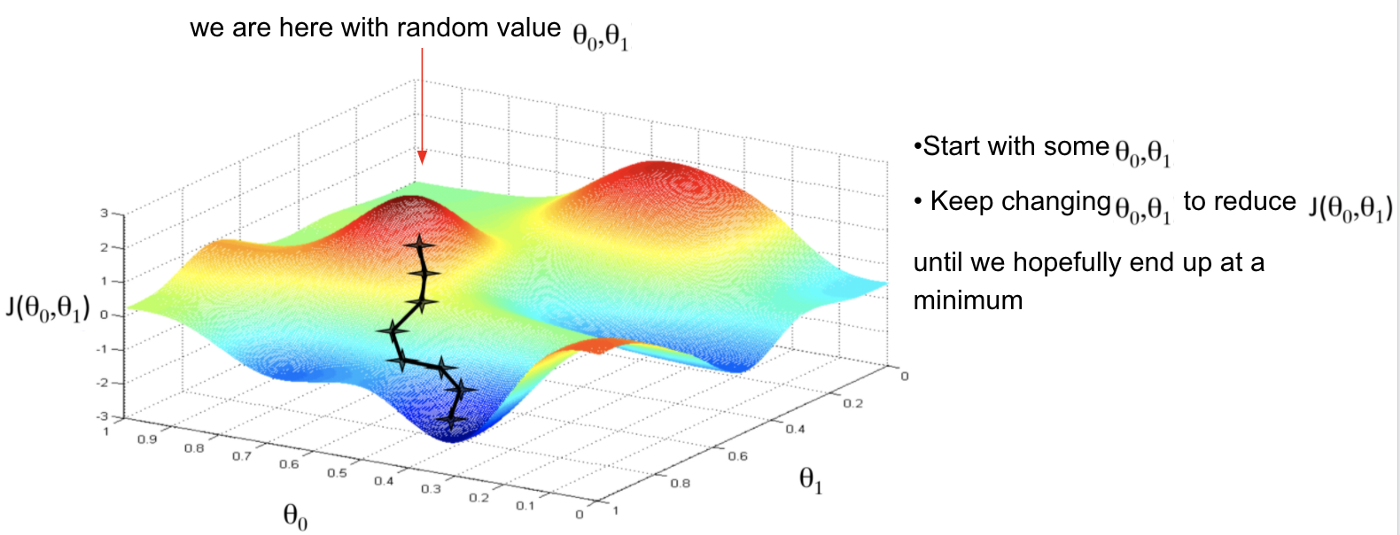
\includegraphics[width=0.9\linewidth]{images/approaches/deep_learning/grad_descent.png}
	\caption{Visualization of the gradient descent algorithm. $\theta_0$ and $\theta_1$ represent the parameters to update: the bias and the weight values, respectively.}
	\label{fig:grad-descent}
\end{figure}


\FloatBarrier
%%%%%%%%%%%%%%%%%%%%%%%%%%%%%%%%%%%%%%%%%%%%%%%%%%%%%%%%%%%%%%%%%%%%%%%%
\subsubsection*{Convolutions in Neural Networks}
%%%%%%%%%%%%%%%%%%%%%%%%%%%%%%%%%%%%%%%%%%%%%%%%%%%%%%%%%%%%%%%%%%%%%%%%

A Convolutional Neural Network (CNN) has the same architecture as the usual Neural Network but arranges its neurons in three dimensions (width, height, depth). Every layer of a CNN transforms the 3D input volume to a 3D output volume of neuron activations.
There are three typologies of layers utilized in a CNN architecture: the convolutional layer, which increases the efficiency of the forward function and vastly reduces the number of parameters, the pooling layer, and the fully-connected layer, which is the regular layer present in Neural Networks.
Typically convolutional layers are followed by an activation function, such as a ReLU.
The convolutional and pooling layers are used for feature extraction, while the fully connected layers are used for classification. An architecture overview is displayed in \autoref{fig:cnn-arch}.

\begin{figure}[h]
	\centering
	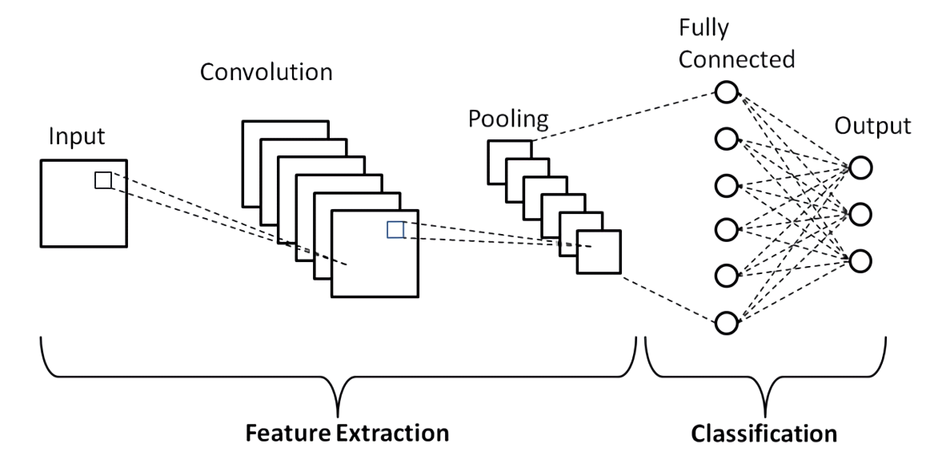
\includegraphics[width=0.9\linewidth]{images/approaches/deep_learning/cnn_arch.png}
	\caption{Overview of a CNN architecture.}
	\label{fig:cnn-arch}
\end{figure}

The \textbf{Convolutional layer}’s parameters consist of a set of learnable filters. Every filter is small spatially (along width and height) but extends through the full depth of the input volume.
A typical filter on the first layer of a Convolutional Neural Network might have size 5x5x3 because colored images have depth 3, the color channels.
During the forward pass, each filter is slid across the width and height of the input volume. The dot products between the entries of the filter and the input at any position are computed.
As the filter slides over the width and height of the input volume, it produces a 2-dimensional activation map that represents the responses of that filter at every spatial position.
In this way, the network will learn filters that activate when they see some type of visual features, such as an edge.
Inside a convolutional layer, there is a set of filters: each of them extracts a particular feature and produces a separate 2-dimensional activation map.
These activation maps are stacked along the depth dimension and produce the output volume.

The first advantage of a convolutional layer is the \textbf{local connectivity} (depicted in \autoref{fig:cnn-local}): each neuron of the layer is connected only to a local region of the input volume.
The spatial extent of this connectivity is a hyperparameter called the receptive field of the neuron (equivalently this is the filter size). The connections are local in 2D space (along width and height) but always full along with the entire depth of the input volume.

The second advantage is \textbf{parameter sharing}.
It is possible to dramatically reduce the number of parameters by making one reasonable assumption: if one feature is useful to compute at some spatial position (x,y), then it should also be useful to compute at a different position (x2,y2).
A practical application of this reasoning can be found in \autoref{fig:cnn-filters}.
The parameter sharing is done by slicing the depth of the volume size into 2-dimensional slices, called depth slices. The neurons in each depth slice share the same weights and bias.
For example, a volume of size 55x55x96 has 96 depth slices, each of size 55x55; by using a filter size of 11x11x3 on the volume, the convolutional layer will have only 96 unique sets of weights for a total of $96*11*11*3 = 34\,848$ unique weights, or $34\,944$ parameters (+$96$ biases).
Without this technique, the parameters would have been much more: $96*55*55 = 290\,400$ neurons, each using $11*11*3 = 363$ weights and $1$ bias, for a total of $290\,400 * 364 = 105\,705\,600$ parameters.
During backpropagation, every neuron in the volume will compute the gradient for its weights, but these gradients will be added up across each depth slice, and only update a single set of weights per slice.

\begin{figure}[!h]
     \centering
     \begin{subfigure}[b]{0.45\textwidth}
         \centering
         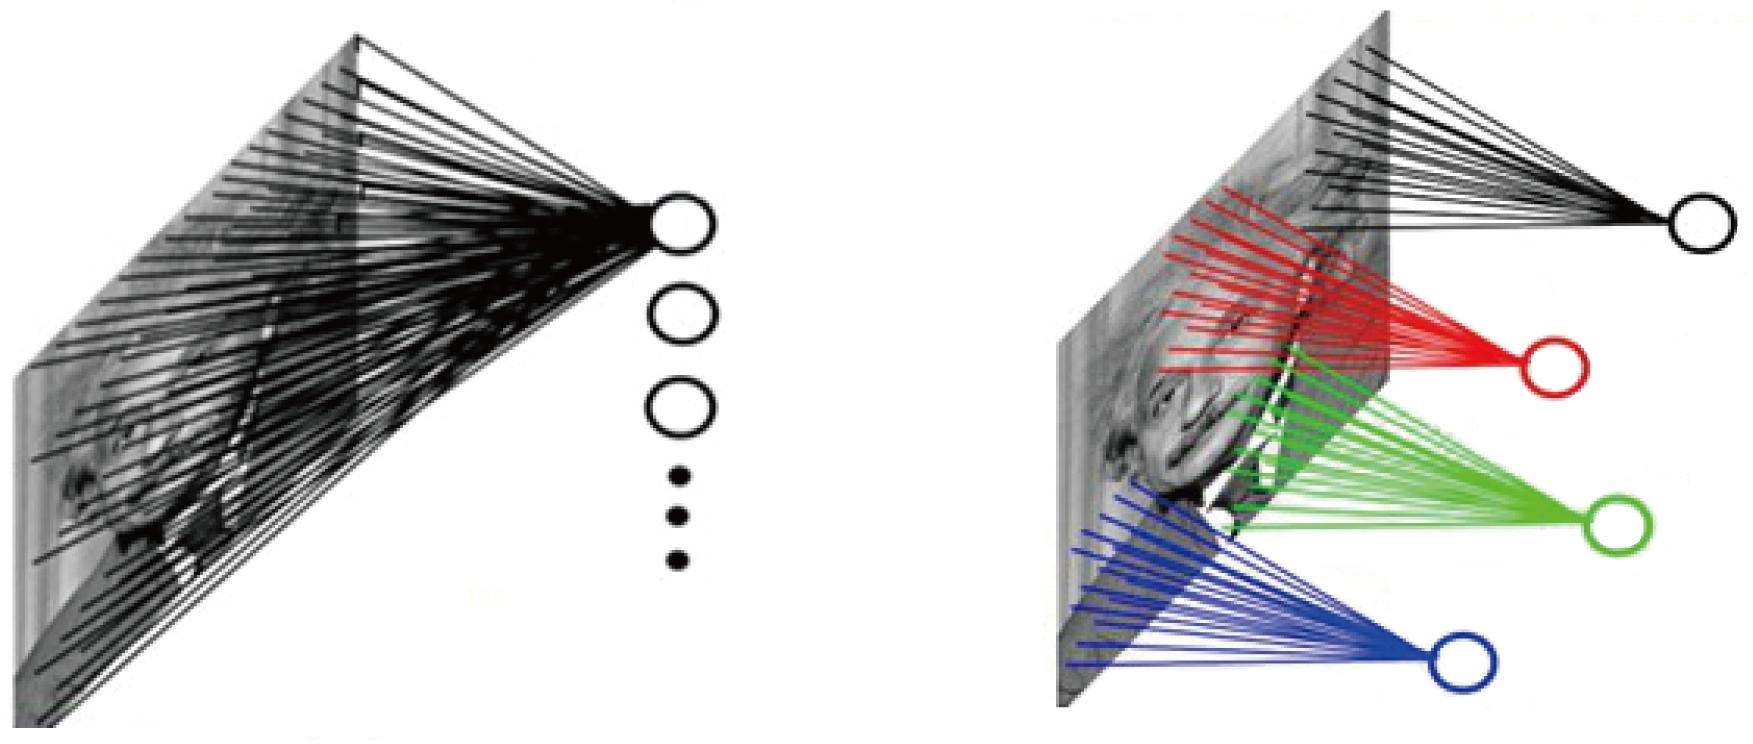
\includegraphics[width=\textwidth]{images/approaches/deep_learning/cnn_local.png}
         \caption{}
         \label{fig:cnn-local}
     \end{subfigure}
     \hfill
     \begin{subfigure}[b]{0.45\textwidth}
         \centering
         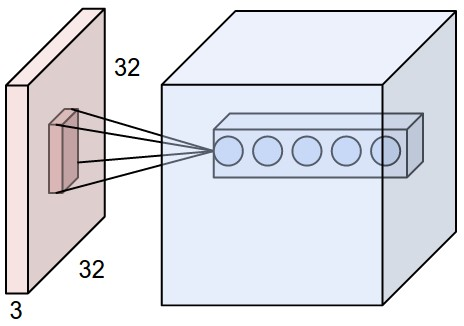
\includegraphics[width=\textwidth]{images/approaches/deep_learning/conv_filter_depth.jpeg}
         \caption{}
         \label{fig:cnn-filter-depth}
     \end{subfigure}
        \caption{Some Convolutional layer features. (a) Global (left) and local (right) perception.
        (b) The red volume represents an example input, a 32x32x3 image, and the blue volume is an example volume of neurons in the first Convolutional layer.
        Each neuron in the convolutional layer is connected only to a local region in the input volume spatially, but to the full depth (all color channels).
        Note, there are multiple neurons (5 in this example) along with the depth, all looking at the same region in the input: these neurons share the same receptive field.
        Despite this, they do not share the same weights, because they are associated with 5 different filters.}
        \label{fig:cnn-features-1}
\end{figure}

\begin{figure}[h]
	\centering
	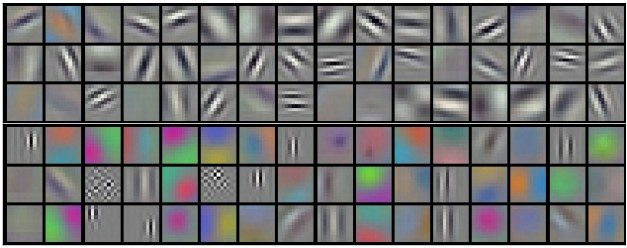
\includegraphics[width=0.9\linewidth]{images/approaches/deep_learning/filters.jpeg}
	\caption{Example filters adapted from Krizhevsky \textit{et al.} 2012~\cite{krizhevsky2012imagenet}.
	Each of the 96 filters shown here is of size [11x11x3], and each one is shared by the 55*55 neurons in one depth slice.
	Notice that the parameter sharing assumption is relatively reasonable: if detecting a horizontal edge is important at some location in the image, it should intuitively be useful at some other location as well.
	There is therefore no need to relearn to detect a horizontal edge at every one of the 55*55 distinct locations in the Conv layer output volume.}
	\label{fig:cnn-filters}
\end{figure}

It is common to periodically insert a \textbf{Pooling layer}, which performs a form of non-linear down-sampling, in-between successive Convolutional layers in a CNN architecture.
Its function is to progressively reduce the spatial size of the representation to reduce the number of parameters and computation in the network, and hence to also control overfitting.
There are several non-linear functions to implement pooling, where max pooling is the most common (depicted in \autoref{fig:max-pool}.
It partitions the input image into a set of rectangles and, for each such sub-region, outputs the maximum.
It is important to note that pooling loses the precise spatial relationships between high-level parts (such as nose and mouth in a face image).

\begin{figure}[h]
	\centering
	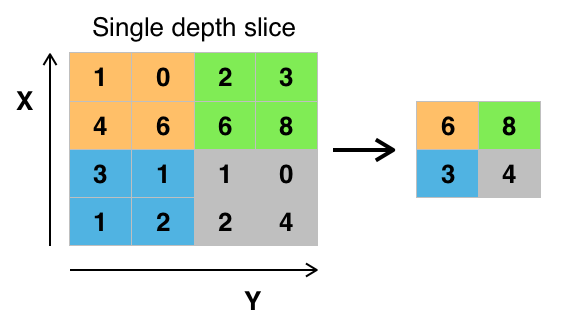
\includegraphics[width=0.7\linewidth]{images/approaches/deep_learning/Max_pooling.png}
	\caption{Max pooling with a 2x2 filter and stride = 2: the filter moves two pixels right for each horizontal movement and two pixels down for each vertical movement.}
	\label{fig:max-pool}
\end{figure}

\FloatBarrier
%%%%%%%%%%%%%%%%%%%%%%%%%%%%%%%%%%%%%%%%%%%%%%%%%%%%%%%%%%%%%%%%%%%%%%%%
\subsection{Implementation}\label{sec:impl-unet}
%%%%%%%%%%%%%%%%%%%%%%%%%%%%%%%%%%%%%%%%%%%%%%%%%%%%%%%%%%%%%%%%%%%%%%%%

%% SPIEGO MODELLO SCELTO
The chosen implementation\footnote{Source code available at \url{https://github.com/ttarasiewicz/Skinny}} consists of a modified U-Net~\cite{ronneberger2015u} incorporating dense blocks and inception modules to benefit from a wider spatial context.
The network is named Skinny~\cite{tarasiewicz2020skinny} and is depicted in \autoref{fig:skinny-arch}.
An additional deep level is appended to the original U-Net model, to better capture large-scale contextual features in the deepest part of the network.
The features extracted in the contracting path propagate to the corresponding expansive levels through the dense blocks.
The original U-Net convolutional layers are replaced with the inception modules: before each max-pooling layer, in the contracting path, and after concatenating features, in the expanding path.
Thanks to these architectural choices, Skinny benefits from a wider pixel context.

\begin{figure}[h]
	\centering
	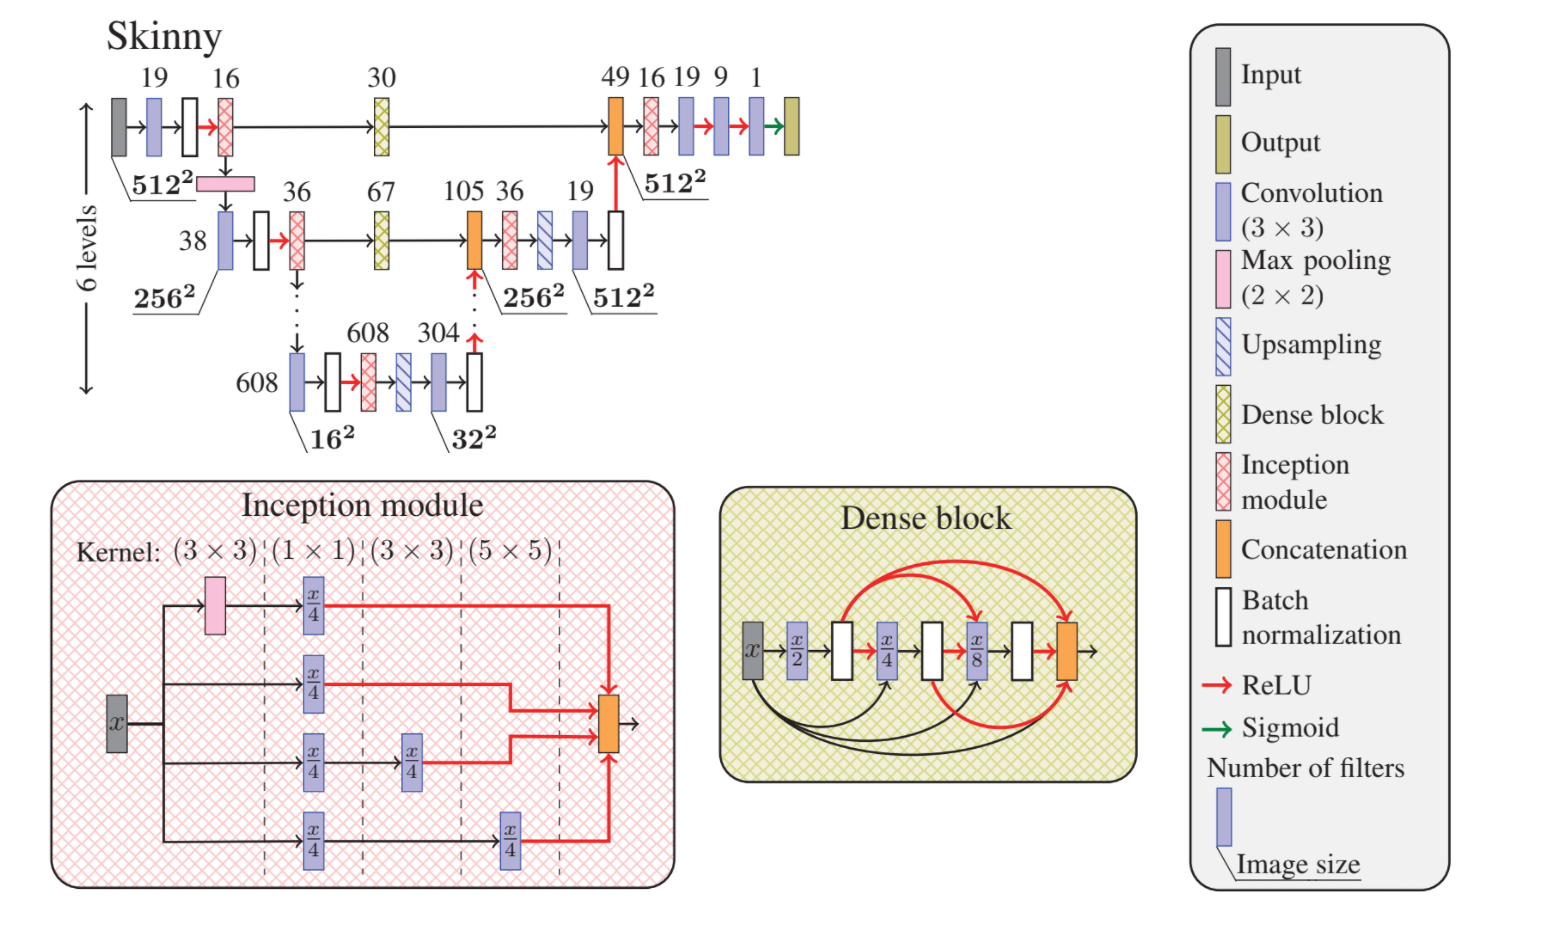
\includegraphics[width=0.9\linewidth]{images/approaches/deep_learning/skinny_arch.png}
	\caption{The architecture of Skinny.
	Adapted from Tarasiewicz \textit{et al.} 2020~\cite{tarasiewicz2020skinny}}
	\label{fig:skinny-arch}
\end{figure}


%% SPIEGO NEL DETTAGLIO
\noindent In image segmentation, it would be useful for the output of a Neural Network to be directly a classification map.
It can be achieved by decapitating the fully connected layers of a CNN network, converting it into a \textbf{Fully Convolutional Network (FCN)}~\cite{long2015fully}.
In fact, fully connected layers can be viewed as convolutions with kernels that cover their entire input regions.
An example of a fully convolutional network is the \textbf{U-Net}~\cite{ronneberger2015u} (called in this way because of its U shape, which can be seen in \autoref{fig:enc-dec}), a famous network used for semantic segmentation.
The architecture of an FCN can be seen as a union of two networks: an encoder, which takes the input and output a feature map, and a decoder, which takes the feature vector from the encoder and gives a classification map in output.

\begin{figure}[h]
	\centering
	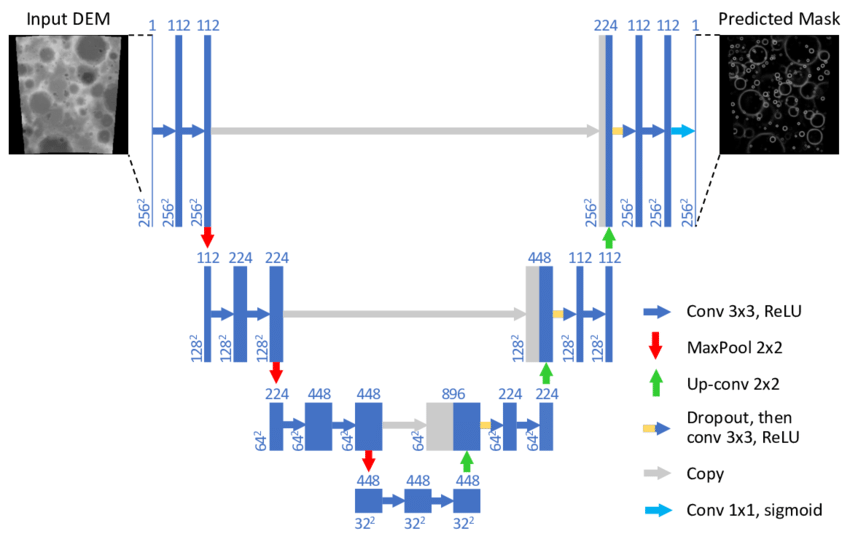
\includegraphics[width=0.9\linewidth]{images/approaches/deep_learning/unet_arch.png}
	\caption{U-Net is a Fully Convolutional Network that utilizes the encoder-decoder architecture.
	The encoder consists of the contracting pathway of the network, while the decoder consists of the expanding pathway.
	Adapted from Silburt \textit{et al.} 2019~\cite{silburt2019lunar}}
	\label{fig:enc-dec}
\end{figure}

The encoder performs the feature extraction task via multiple down-sampling operations, in the same way as the first part of a CNN.
The decoder must then up-sample these feature maps multiple times until the achievement of the desired classification map, which size is determined by the architecture.
The upsampling operation is possible thanks to the skip connections.
\textbf{Skip connections} are used to skip features from the contracting path to the expanding path in order to recover spatial information lost during downsampling, making fully convolutional methods suitable for semantic segmentation.
The \textbf{Up-sampling layer} consists of a transposed convolution, an operation that goes in the opposite direction to a convolution, as shown in \autoref{fig:deconv}.

\begin{figure}[h]
	\centering
	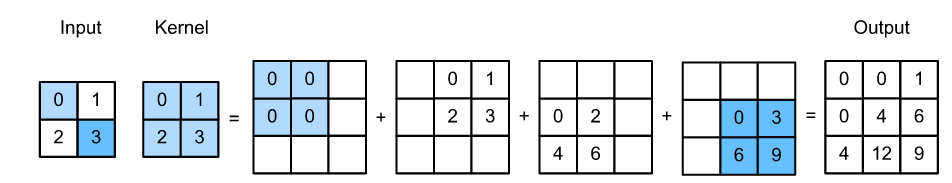
\includegraphics[width=0.9\linewidth]{images/approaches/deep_learning/deconv_w.png}
	\caption{Transposed convolution. Each element of the input feature map is taken and multiplied with every element of the kernel. The outputs of these operations are then summed.}
	\label{fig:deconv}
\end{figure}

The main advantage of the chosen implementation compared to a regular U-Net is the addition of inception modules and dense blocks.
Salient parts in the image can have extremely large variations in size.
For example, an image can represent a dog nearby or far away, and the size of the part of the image occupied by the dog varies.
Because of the huge variation in the location of the information, choosing the right kernel size for the convolution operation becomes tough.
A larger kernel is preferred for information distributed more globally, and a smaller kernel is preferred for information distributed more locally.
The solution is to have filters with multiple sizes operate on the same level. The \textbf{inception module}~\cite{szegedy2015going} (displayed in \autoref{fig:inception}) performs this operation.

\textbf{Dense blocks}~\cite{huang2017densely} strengthen feature propagation and reuse.
A dense block comprises $n$ dense layers. These dense layers are connected using a dense circuitry such that each dense layer receives feature maps from all preceding layers and passes its feature maps to all subsequent layers.
The dimensions of the features (width, height) stay the same in a dense block, but the number of filters changes between them.
A dense layer can be imagined as a convolutional layer, followed by a batch normalization layer, and the activation function.

The goal of \textbf{Batch Normalization}~\cite{ioffe2015batch} is to achieve a stable distribution of activation values throughout training.
The distribution of the inputs to layers somewhere down in the network may change after each mini-batch of input images, as the weights refresh.
This can make the learning algorithm always pursue a moving target.
In a neural network, batch normalization is achieved through a normalization step that fixes the means and variances of each layer's inputs.
Ideally, the normalization would be conducted over the entire training set.
However, to use this step jointly with optimization methods, it is impractical to use global information.
Thus, normalization is restrained to each mini-batch in the training process.

\begin{figure}[h]
     \centering
     \begin{subfigure}[b]{0.45\textwidth}
         \centering
         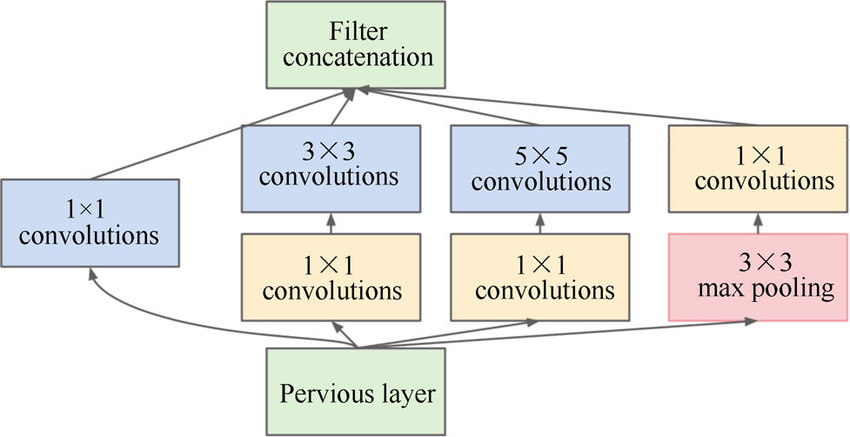
\includegraphics[width=\textwidth]{images/approaches/deep_learning/inception_mod.png}
         \caption{}
         \label{fig:inception}
     \end{subfigure}
     \hfill
     \begin{subfigure}[b]{0.45\textwidth}
         \centering
         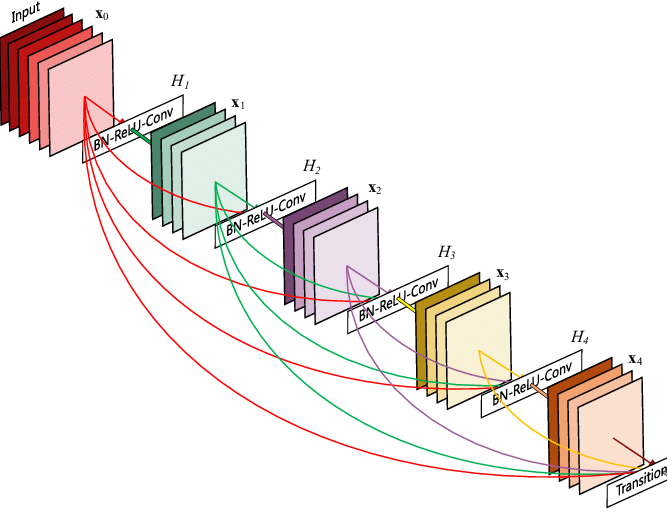
\includegraphics[width=\textwidth]{images/approaches/deep_learning/dense_block.png}
         \caption{}
         \label{fig:dense-block}
     \end{subfigure}
        \caption{(a) Inception module. 1x1 convolutions reduce the dimension along the direction of the number of channels, making the process less computationally expensive.
        Adapted from Szegedy \textit{et al.} 2015~\cite{szegedy2015going}.
        (b) A 5-layer dense block with a growth rate of k = 4.
        Every layer has access to its preceding feature maps, and therefore, to the collective knowledge.
        Each layer adds then new information to this collective knowledge, in concrete k feature maps of information.
        Adapted from Huang \textit{et al.} 2017~\cite{huang2017densely}.}
        \label{fig:inception-dense}
\end{figure}



  %%%%%%%%%%%%%%%%%%%%%%%%%%%%%%%%%%%%%%%%%%%%%%%%%%%%%%%%%%%%%%%%%%%%%%%%
\chapter{Results}\label{chap:results}
%%%%%%%%%%%%%%%%%%%%%%%%%%%%%%%%%%%%%%%%%%%%%%%%%%%%%%%%%%%%%%%%%%%%%%%%

% cosa metto qui? magari la parte delle metriche?

%%%%%%%%%%%%%%%%%%%%%%%%%%%%%%%%%%%%%%%%%%%%%%%%%%%%%%%%%%%%%%%%%%%%%%%%
\section{Metrics}
%%%%%%%%%%%%%%%%%%%%%%%%%%%%%%%%%%%%%%%%%%%%%%%%%%%%%%%%%%%%%%%%%%%%%%%%

Metrics give accurate measurements about how a process is functioning and provide a measure to suggest the improvements.
Developing and understanding standardized metrics is crucial to guide decision-making and prevent the need to make hasty decisions~\cite{austin2021need}.

As stated in \ref{sec:state-of-the-art}, skin detection is a two-class problem.
To evaluate a binary classifier, the ideal data (the ground truth) is compared to the predicted data given by the method.
In the case of skin detection, data is generally represented by binary masks.
The primitive metrics to define are the ones inside a confusion matrix, depicted in \autoref{fig:confmat}.
A \textbf{False Positive} is an error in binary classification in which a test result incorrectly indicates the presence of a condition such as a disease when the disease is not present.
A \textbf{False Negative} represents the opposite case: the test result incorrectly fails to indicate the presence of a condition when it is present.
These are the two kinds of errors in a binary test, in contrast to the two kinds of correct results (a \textbf{True Positive} and a \textbf{True Negative}).
It is important to note that the gravity of an error depends on the contest. %In the medical field, a False Negative may represent a bigger problem than a False Positive 
An example of different error seriousness is illustrated in \autoref{fig:bin-errors}.
In image segmentation, False Positives may represent a lesser gravity since a follow-up processing of the image could fix the issues, while the data of false negatives is lost.

\begin{figure}[h]
    \centering
    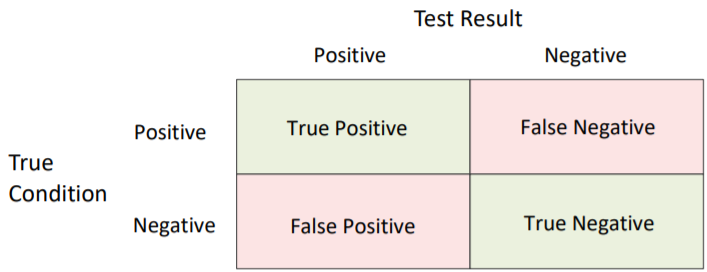
\includegraphics[width=0.7\linewidth]{images/results/confmat.png}
    \caption{A confusion matrix.}
    \label{fig:confmat}
\end{figure}

\begin{figure}[h]
    \centering
    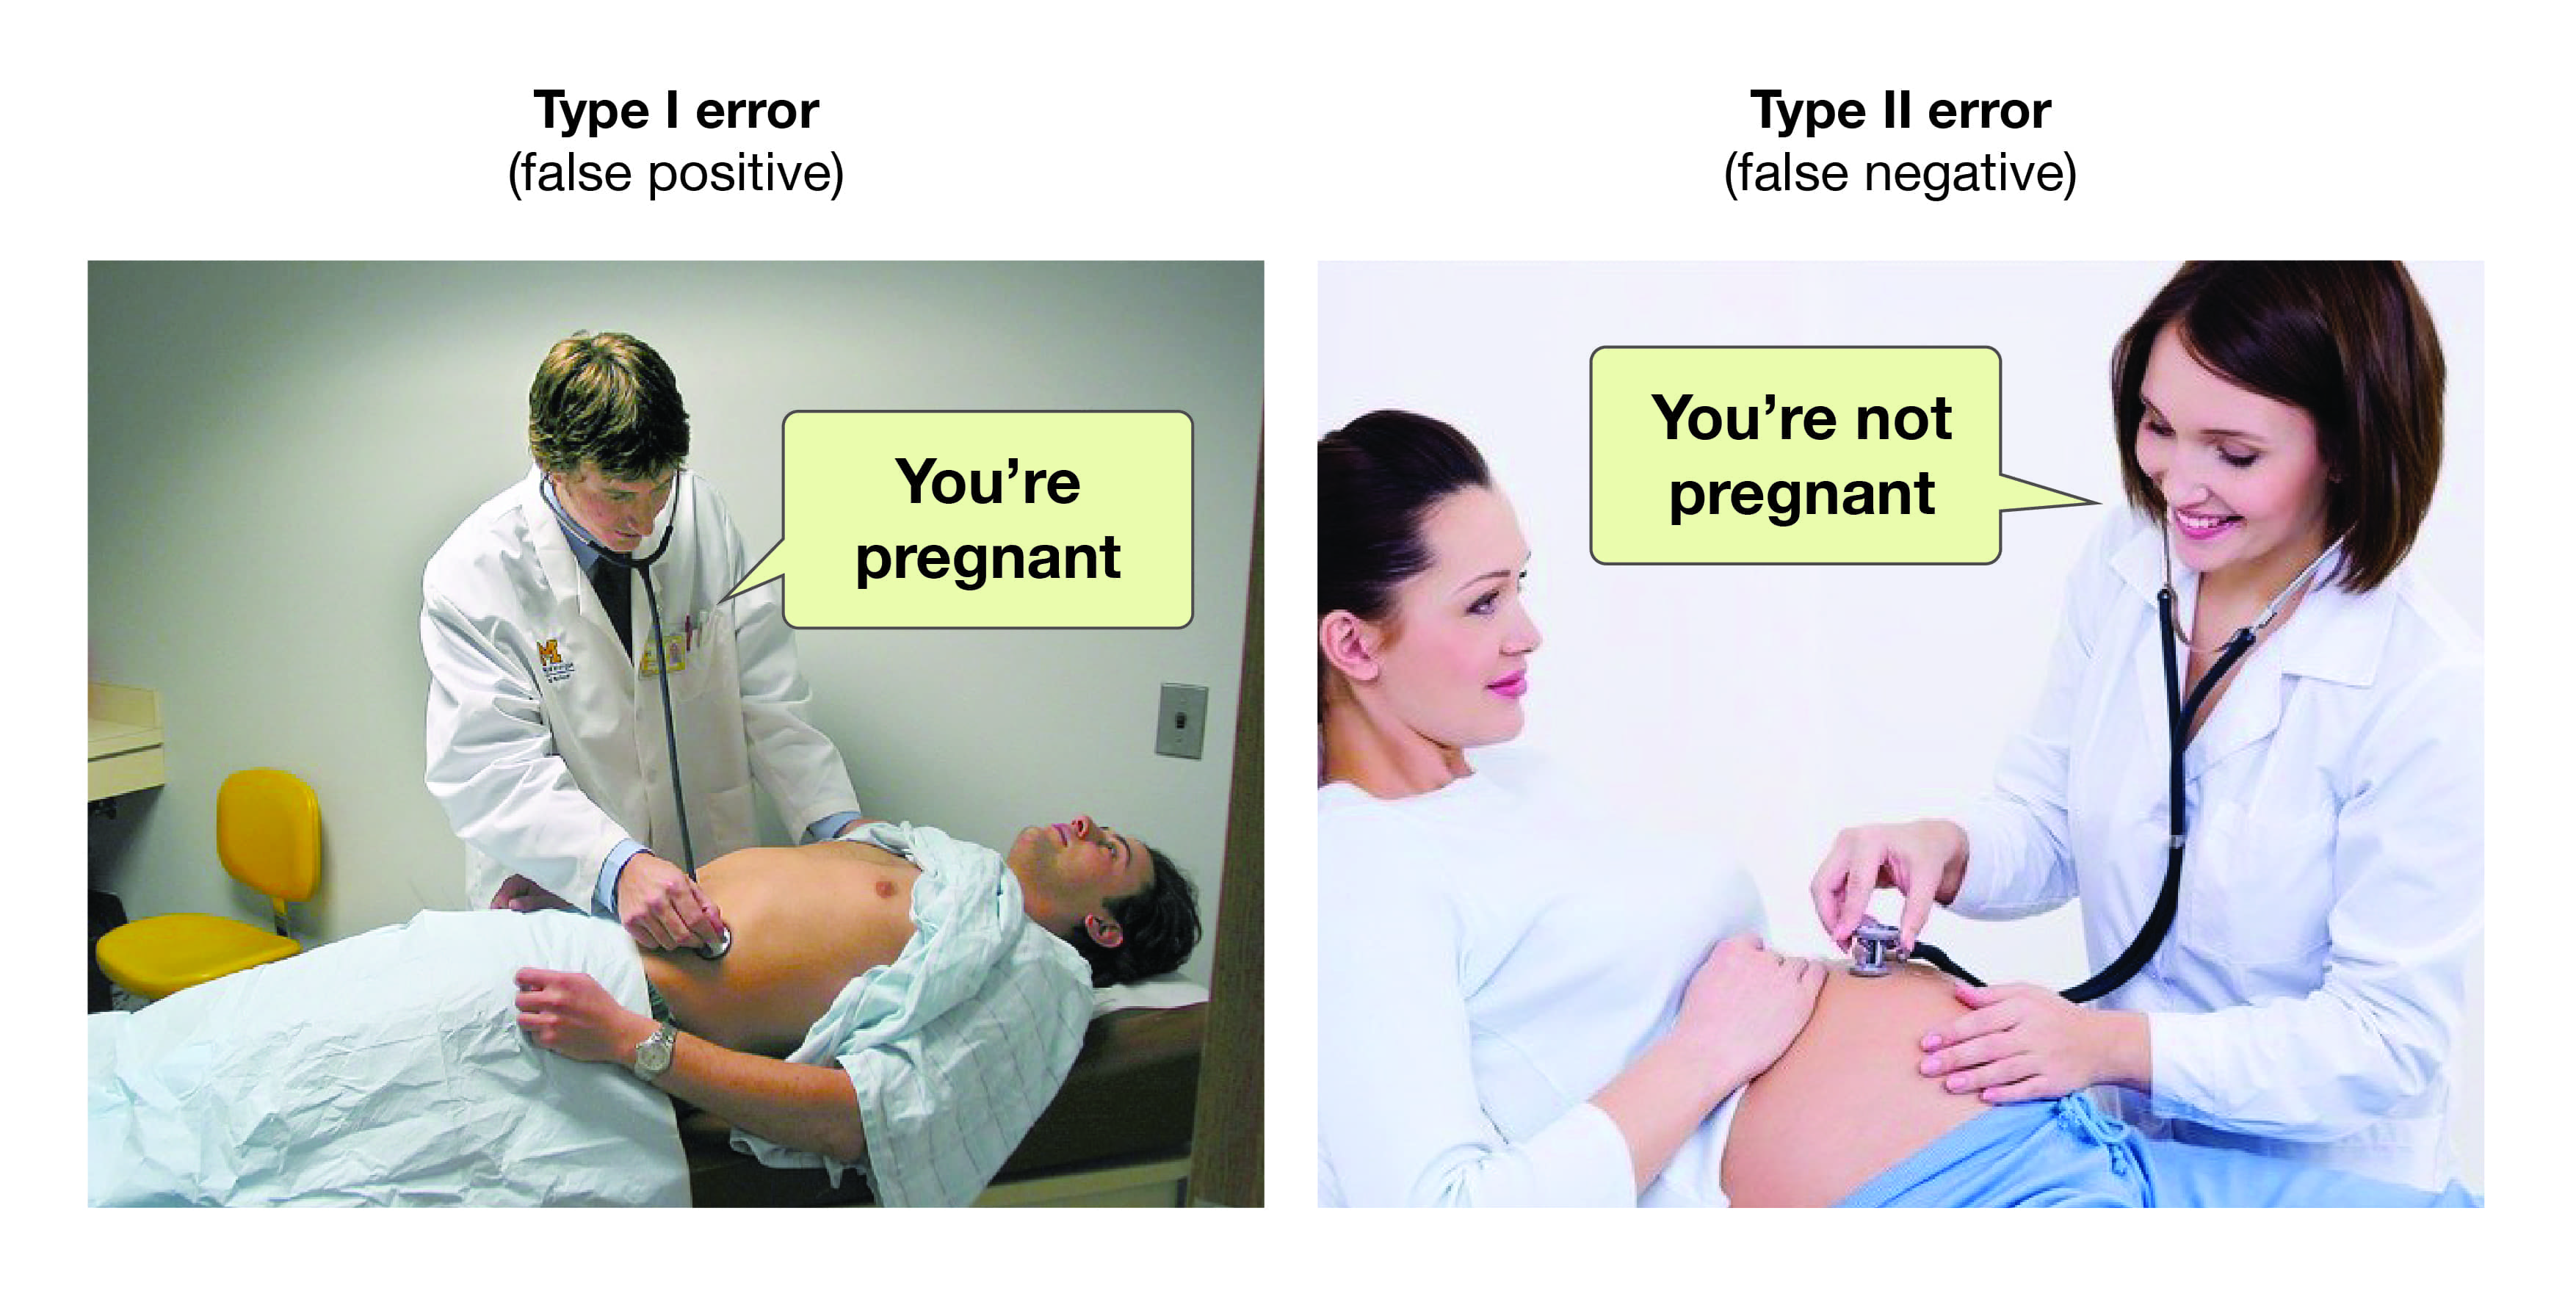
\includegraphics[width=0.9\linewidth]{images/results/bin_type_errors.jpeg}
    \caption{The gravity of an error depends on the contest in which it happens. False Negatives and False Positives can have different gravity.}
    \label{fig:bin-errors}
\end{figure}

Starting from the primitive metrics, it is possible to compute more complex evaluation metrics, such as Recall, Specificity, and Precision.\\
\textbf{Recall}, also called True Positive Rate or Sensitivity, represents how many relevant items are selected.\\
\textbf{Specificity}, also called False Positive Rate, represents how many negative elements are truly negative.\\
\textbf{Precision} represents how many selected items are relevant.\\
These metrics are calculated as follows:

\begin{equation}
    \begin{aligned}
    Recall &= \frac{TP}{TP + FN}\\[10pt]
    Specificity &= \frac{TN}{TN + FP}\\[10pt]
    Precision &= \frac{TP}{TP + FP}\\[10pt]
    \end{aligned}
\end{equation}

where $TP, TN, FP, FN$ are respectively True Positives, True Negatives, False Positives, and False Negatives.

\noindent Recall, Specificity, and Precision may not be enough to evaluate a classifier, so they are often combined into other metrics, such as F\textsubscript{1}-Score, IoU, and D\textsubscript{prs}.\\
\textbf{F\textsubscript{1}-Score}, also called F-Measure, Sørensen-Dice coefficient, or Dice similarity coefficient, is a measure of a test's accuracy.
The F\textsubscript{1} in its name means that the $\beta$ value of the generic F-Score is set to 1.
The $F_1$ score is the harmonic mean of precision and recall.
The more generic $F_\beta$ score applies additional weights, valuing one of precision or recall more than the other.\\
\textbf{Intersection Over Union (IoU)}, also named Jaccard index, measures similarity between finite sample sets, and is defined as the size of the intersection divided by the size of the union of the sample sets. The sample sets are represented by the ground truth and the prediction given by a skin detector.\\
\textbf{D\textsubscript{prs}}~\cite{intawong2013new} is a metric that focuses on segmentation algorithms. The already mentioned metrics are expressed as a compromise between two of the three aspects that are important for a quality assessment: Precision, Recall, and Specificity~\cite{intawong2013new}.
D\textsubscript{prs} takes into account all of the three aspects.
It measures the Euclidean distance between the segmentation, represented by the point $(PR, RE, SP)$, and the ground truth, the ideal point $(1, 1, 1)$, hence lower values are better in this case.\\
These metrics are calculated as follows:

\begin{equation}
    \begin{aligned}
    F_1&=\frac{2 T P}{2 T P+F P+F N}\\[10pt]
    IoU&=\frac{T P}{T P+F P+F N}\\[10pt]
    D_{p r s}&=\sqrt{(1-P R)^{2}+(1-R E)^{2}+(1-S P)^{2}}\\[10pt]
    \end{aligned}
\end{equation}

where $PR, RE, SP$ are Precision, Recall, and Specificity, respectively.

\noindent It is possible to note that F\textsubscript{1}-Score and IoU have a similar formula: the only difference is that  F\textsubscript{1} weights the True Positives higher.
When taking the average score of each metric over a set of inferences, IoU tends to penalize single instances of bad classification more than the F\textsubscript{1} score~\footnote{A detailed explanation can be found at \url{https://stats.stackexchange.com/a/276144}}.
Suppose for example that the vast majority of the inferences are moderately better with classifier A than B, but some of them are significantly worse using classifier A. It may be the case then that the F\textsubscript{1} metric favors classifier A while the IoU metric favors classifier B.
For a better interpretation of the average scores between multiple instances, the difference \textbf{F\textsubscript{1}-IoU} is taken into account.
The higher the difference, the more is the bad inferences in the set, while a lower difference means that the prediction set is more balanced.
All the described metrics range from 0 to 1, except for primitives, which are whole numbers, and D\textsubscript{prs}, which ranges from 0 to $\sqrt{3}$.

\noindent It is also important to note that F\textsubscript{1} and IoU do not take into account the True Negatives. In the case of skin detection the performances are generally measured on the skin class, hence this limitation is negligible. However, if True Negatives are important for an evaluation, more balanced metrics should be taken into account, such as the Matthews correlation coefficient (MCC)~\cite{chicco2020advantages}.


%%%%%%%%%%%%%%%%%%%%%%%%%%%%%%%%%%%%%%%%%%%%%%%%%%%%%%%%%%%%%%%%%%%%%%%%
\section{Experimental setup}
%%%%%%%%%%%%%%%%%%%%%%%%%%%%%%%%%%%%%%%%%%%%%%%%%%%%%%%%%%%%%%%%%%%%%%%%

% VALIDATION
Before the evaluation process on the chosen datasets, the selected methods have been validated on the datasets splits used in their original papers.
In this way, it has been possible to check their proper functioning.
The statistical method~\cite{acharjee2018skin} has not been validated because it does not refer to a paper and evaluations are not reported.
The thresholding method~\cite{brancati2017human} uses a metrics averaging of this type: the Recall, Precision, and Specificity measures are calculated as average scores over the set of instances, then the obtained scores are used to calculate F\textsubscript{1}-Score and D\textsubscript{prs}.
The U-Net approach~\cite{tarasiewicz2020skinny}, instead, calculates the F\textsubscript{1}-Score directly as the average score over all the set of instances.
The validation results are shown in \autoref{tab:methods-val-dyc}
and \autoref{tab:methods-val-skinny}.

\begin{table}[h]
    \centering
    \resizebox{\columnwidth}{!}{
        \begin{tabular}{l@{\hskip 12mm}ccc@{\hskip 8mm}ccc}
        \toprule
        & \multicolumn{3}{c}{F\textsubscript{1}-Score} & \multicolumn{3}{c}{D\textsubscript{prs}}\\
        & HGR\textsuperscript{1} & ECU & Pratheepan & HGR\textsuperscript{1} & ECU & Pratheepan\\
        \midrule
        Original & \monosp{0.8252} & \monosp{0.6550} & \monosp{0.6592} & \monosp{0.2667} & \monosp{0.5043} & \monosp{0.5149}\\
        Implementation & \monosp{0.8257} & \monosp{0.6586} & \monosp{0,6630} & \monosp{0.2660} & \monosp{0.5006} & \monosp{0.5096}\\
        \midrule
        Change & \monosp{0.0005} & \monosp{0.0036} & \monosp{0.0038} & \monosp{0.0007} & \monosp{0.0037} & \monosp{0.0053}\\
        \bottomrule
        \end{tabular}}
    \caption{Brancati \textit{et al.} 2017~\cite{brancati2017human} validation data.\\
    Each dataset was used in its entirety to perform the testing.\\
    \textsuperscript{1}HGR consists of: HGR1, HGR2A-downscaled, HGR2B-downscaled.}
    \label{tab:methods-val-dyc}
\end{table}

\begin{table}[h]
    \centering
    %\resizebox{\columnwidth}{!}{
        \begin{tabular}{l@{\hskip 12mm}cc}
        \toprule
        & \multicolumn{2}{c}{F\textsubscript{1}-Score}\\
        & HGR\textsuperscript{1} & ECU\textsuperscript{2}\\
        \midrule
        Original & \monosp{0.9494} & \monosp{0.9230}\\
        Implementation & \monosp{0.9308}  & \monosp{0.9133}\\
        \midrule
        Change & \monosp{0.0186} & \monosp{0.0097}\\
        \bottomrule
        \end{tabular}%}
    \caption{Tarasiewicz \textit{et al.} 2020~\cite{tarasiewicz2020skinny} validation data.\\
    \textsuperscript{1}HGR consists of: HGR1, HGR2A-downscaled, HGR2B-downscaled.\\
    \textsuperscript{2}ECU was split accordingly to the original work of the method.\\
    The model was trained on the ECU splits; HGR has not been used for training.\\
    The testing was performed on the test set of ECU and the entirety of HGR.}
    \label{tab:methods-val-skinny}
\end{table}


% DATASETS
After the validation phase, the setup of the experiments begins with the definition of the employed datasets:
\begin{itemize}
    \item ECU: 3998 images.
    \item HGR: 1558 images from HGR1, HGR2A-downscaled, HGR2B-downscaled sub-datasets.
    \item Schmugge: 840 images.
    The pictures have been processed by reading the \path{.config.SkinImManager} file provided by the dataset.
    Five pictures have been ignored because of faulty ground truths: \path{aa50.gt.d3}, \path{dd71.gt.d3}, \path{hh54.gt.d3}, and \path{aa69.gt.d3} that has a duplicated entry in the file.
    The rule used to manage the ternary ground truths has been considering whatever is not the background as skin.
\end{itemize}

\noindent Skin tones sub-datasets are defined by taking advantage of the additional labels in the Schmugge dataset.
The resulting sub-datasets represent light, medium, and dark skin tones and consist of 409, 101, and 27 pictures, respectively.
Not all Schmugge dataset is used for skin tones, because the database contains whole images of non-skin pixels, as described in \autoref{sec:chosen-datasets}.

None of the datasets provide native training and testing splits.
The train and validation sets have been merged in methods that do not use the validation set.
For ECU, the splits used are the ones mentioned in Tarasiewicz \textit{et al.} 2020~\cite{tarasiewicz2020skinny}.
HGR, Schmugge, and skin tone splits are randomly defined by keeping the following proportions: 70\% train, 15\% validation, and 15\% test.
Since the proportions would reduce the dark sub-dataset to only 19 training images, the data has been augmented in this case, only for the training split.
The purpose is to get at least 100 images for the evaluations, but also to generate images that look natural; 104 was the final size of the training set.
The following augmentation operations provided by the Albumentations library~\cite{buslaev2020albumentations} are performed in the following order:
\begin{itemize}
\itemsep0em
    \item \path{HorizontalFlip(p=1)} on original images.
    \item \path{Rotate(limit = 15, p=0.8)} on the original images plus the ones obtained by the horizontal flipping.
    \item \path{RandomCrop(H*0.8, W*0.8, p=0.8)} on the original images plus the ones obtained by the horizontal flipping plus the ones obtained by the rotation.
\end{itemize}
where \path{H} and \path{W} are the height and width of the processed image, respectively, and \path{p} and \path{limit} are the probability that the transformation happens, and the rotation limits in degrees (the angle is between \path{-limit} and \path{+limit}), respectively.


% METHODS
Once the datasets have been defined, the settings of the methods can be adjusted.
The thresholding~\cite{brancati2017human} and statistical~\cite{acharjee2018skin} approaches have been left to their default implementations settings described in \autoref{sec:impl-thresh} and \autoref{sec:impl-bayes}, respectively.
The U-Net approach~\cite{tarasiewicz2020skinny} uses only the complete model named \q{Skinny} with the following settings:
\begin{itemize}
    \item Maximum number of epochs = 200
    \item Batch size = 3
    \item Initial learning rate = $10^{-4}$
    \item Minimum learning rate = $10^{-6}$
    \item Reduce learning rate on plateau patience = 5
    \item Early stopping patience = 10 for HGR, ECU, and Schmugge models.\\
    Early stopping patience = 50 for light, medium, dark models (by having only 4 validation images in the dark sub-dataset, the model has a harder time taking the right path).
    \item Adam~\cite{kingma2014adam} optimizer with $\beta_1 = 0.9$ and $\beta_2 = 0.999$
    \item The loss function is the average of Binary Cross-Entropy and the Dice coefficient.
    \item The original preprocessing: the images with over $(512 \times 512)$ pixels are downscaled preserving the aspect ratio so that the number of pixels does not exceed $(512 \times 512)$. Moreover, Skinny applies a padding operation after the possible downscale to make the width and height of images multiple of 32, as seen in \autoref{fig:skinny-padding}.
    \item The models have been trained by monitoring the F\textsubscript{1} over the validation set and saving on new max values.
\end{itemize}


% EVALUATION
\noindent The last phase of the setup is defining the evaluation process.
Some methods did not provide a binary prediction, but a prediction with grayscale values. All the predictions have been binarized by rounding each pixel value to either be white or black.
%By having a binarized ground truth and a binarized prediction, metrics measurement is possible.
Initially, the metrics are measured for all the instances, then the average and population standard deviation for each metric are computed.

% cross, base, performance
Two different settings of dataset evaluation are performed: single and cross evaluation.
The first measures how well a method performs with respect to the same dataset, the second measures how well a method generalizes with respect to other datasets.\\
In the \textbf{single evaluation} of a method over a dataset, the method is eventually trained on the training set, in the case of a trainable method, and then predictions are performed on the test set.\\
In the \textbf{cross evaluation}, only the trainable approaches are analyzed.
The models are the same of the single evaluation: each model is trained on the training set of a dataset.
The evaluation of a method is performed over the whole dataset by the models that have not been trained on the concerning dataset.

\begin{figure}[h]
     \centering
     \begin{subfigure}[b]{0.23\textwidth}
         \centering
         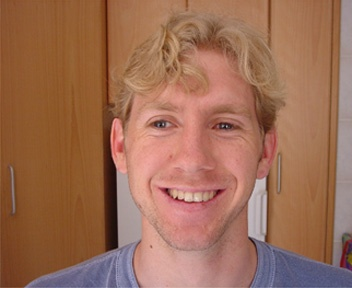
\includegraphics[width=\textwidth]{images/results/unet_padding_im00060_x.jpg}
         \caption{}
     \end{subfigure}
     \hfill
     \begin{subfigure}[b]{0.23\textwidth}
         \centering
         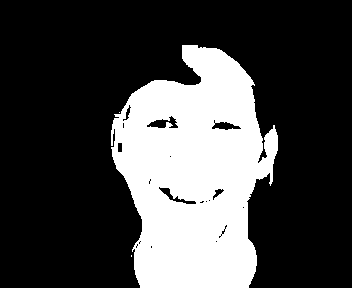
\includegraphics[width=\textwidth]{images/results/unet_padding_im00060_y.png}
         \caption{}
     \end{subfigure}
    \hfill
     \begin{subfigure}[b]{0.23\textwidth}
         \centering
         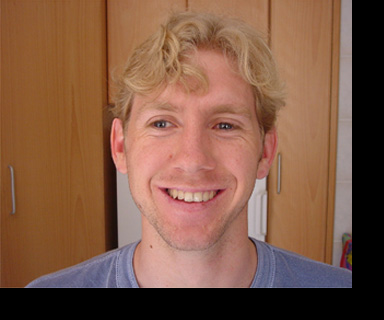
\includegraphics[width=\textwidth]{images/results/unet_padding_1311x.png}
         \caption{}
     \end{subfigure}
    \hfill
     \hfill
     \begin{subfigure}[b]{0.23\textwidth}
         \centering
         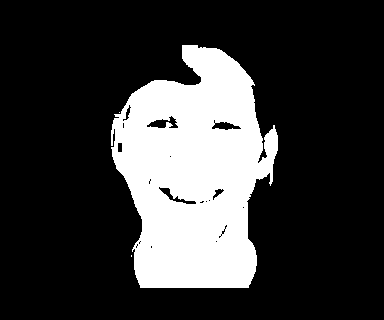
\includegraphics[width=\textwidth]{images/results/unet_padding_1311y.png}
         \caption{}
     \end{subfigure}
        \caption{Skinny~\cite{tarasiewicz2020skinny} applies padding to make the width and height of an image a multiple of 32. If the dimensions of the image are already a multiple of 32, a padding of 32 is still applied.
        (a) original image; (b) ground truth; (c) preprocessed original image; (d) preprocessed ground truth}
        \label{fig:skinny-padding}
\end{figure}


\FloatBarrier
%%%%%%%%%%%%%%%%%%%%%%%%%%%%%%%%%%%%%%%%%%%%%%%%%%%%%%%%%%%%%%%%%%%%%%%%
\section{Performance on single databases}
%%%%%%%%%%%%%%%%%%%%%%%%%%%%%%%%%%%%%%%%%%%%%%%%%%%%%%%%%%%%%%%%%%%%%%%%

In the single evaluation of the datasets, \autoref{tab:base-normal}, the deep-learning approach beats its competitors in all the measurements, while the statistical approach comes always second.
The Schmugge dataset describes a higher difficulty of classification that can be attributed to the variety of the lighting conditions, subjects, and environments present in its pictures.
The variety of the database can also be described by the high standard deviation measurements obtained.
Furthermore, by considering the ambiguous regions as skin pixels, the performance of the classifier may be affected.
The high D\textsubscript{prs} scores obtained by the statistical and thresholding methods may indicate the presence of many True Negatives, as the metric is the only one between the chosen metrics that incorporates them.
HGR seems to be the easier dataset to classify, which can be due to the relatively low diversity of subjects and backgrounds. In fact, learning approaches tend to have very high measurements.
Tarasiewicz \textit{et al.} 2020~\cite{tarasiewicz2020skinny} seems to perform very well on this dataset, achieving very low standard deviation scores.
In the ECU dataset, the results of the histogram and thresholding approaches are relatively close, while the CNN outperforms them by far.

Some interesting instances can be seen in \autoref{fig:base-normal-samples}.
The first row shows the problem that having a background with similar colors to the skin represents in the color-based methods.
The statistical method seems to act relatively better in this scenario compared to Brancati \textit{et al.} 2017~\cite{brancati2017human}, as seen in the second row.
In the third row, the statistical approach classify some background and hair pixels as skin, while the rule-based method has many False Negatives, but the head remain still recognizable.
The fourth row represent a very hard image to classify.
Interestingly, the U-Net describes a very bad classifications, with a tremendous number of False Positives.
The thresholding approach is the most restrictive on False Positives in this instance.
The next-to-last image has an inconvenient background with skin-like colors and only Tarasiewicz \textit{et al.} 2020~\cite{tarasiewicz2020skinny} tend to have a good classification.
The statistical method manages to classify the skin pixels well, but has a really high number of False Positives.
The last image is a landscape image without skin pixels and once again the color-based approaches describe many False Positives, with the machine learning one having lots of them.

\begin{table}[ht]
    \centering
    \resizebox{\columnwidth}{!}{
    \begin{tabular}{clccc}
    \toprule
    & Method\textbackslash Database & ECU & HGR & Schmugge \\
    \midrule
    %
    %
    \multirow{3}{*}{{$F_1 \uparrow$}}
        & Tarasiewicz \textit{et al.}~\cite{tarasiewicz2020skinny}
        & $\pmb{0.9133 \pm 0.08}$ & $\pmb{0.9848 \pm 0.02}$ & $\pmb{0.6121 \pm 0.45}$ \\
        %
        & Acharjee~\cite{acharjee2018skin}
        & $\underline{0.6980 \pm 0.22}$ & $\underline{0.9000 \pm 0.15}$ & $\underline{0.5098 \pm 0.39}$ \\
        %
        & Brancati \textit{et al.}~\cite{brancati2017human}
        & $0.6356 \pm 0.24$ & $0.7362 \pm 0.27$ & $0.4280 \pm 0.34$ \\[5pt]
        %
        %
    \multirow{3}{*}{{$IoU \uparrow$}}
        & Tarasiewicz \textit{et al.}~\cite{tarasiewicz2020skinny}
        & $\pmb{0.8489 \pm 0.12}$ & $\pmb{0.9705 \pm 0.03}$ & $\pmb{0.5850 \pm 0.44}$ \\
        %
        & Acharjee~\cite{acharjee2018skin}
        & $\underline{0.5751 \pm 0.23}$ & $\underline{0.8434 \pm 0.19}$ & $\underline{0.4303 \pm 0.34}$ \\
        %
        & Brancati \textit{et al.}~\cite{brancati2017human}
        & $0.5088 \pm 0.25$ & $0.6467 \pm 0.30$ & $0.3323 \pm 0.28$ \\[5pt]
        %
        %
    \multirow{3}{*}{{$D_{prs} \downarrow$}}
        & Tarasiewicz \textit{et al.}~\cite{tarasiewicz2020skinny}
        & $\pmb{0.1333 \pm 0.12}$ & $\pmb{0.0251 \pm 0.03}$ & $\pmb{0.5520 \pm 0.64}$ \\
        %
        & Acharjee~\cite{acharjee2018skin}
        & $\underline{0.4226 \pm 0.27}$ & $\underline{0.1524 \pm 0.19}$ & $\underline{0.7120 \pm 0.54}$ \\
        %
        & Brancati \textit{et al.}~\cite{brancati2017human}
        & $0.5340 \pm 0.32$ & $0.3936 \pm 0.36$ & $0.8148 \pm 0.48$\\
        %
        %
    \bottomrule
    \end{tabular}}
    \caption{Single evaluation on datasets.\\
        For each dataset: methods are eventually trained on the training set, in the case of trainable methods, and then predictions are performed on the test set.\\
        For example, with ECU as the dataset, it means that a method is trained using the training set of ECU, if the method is trainable, and then tested on the test set of ECU.}
    \label{tab:base-normal}
\end{table}

\begin{figure}[h]
     \centering
     % ROW 1
     \begin{subfigure}[b]{0.18\textwidth}
         \centering
         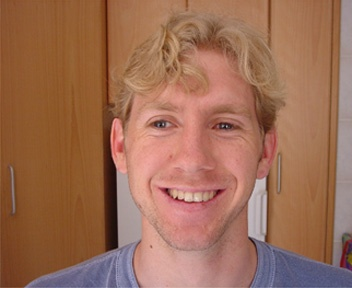
\includegraphics[width=\textwidth]{images/results/base/im00060_x.jpg}
     \end{subfigure}
     \hfill
     \begin{subfigure}[b]{0.18\textwidth}
         \centering
         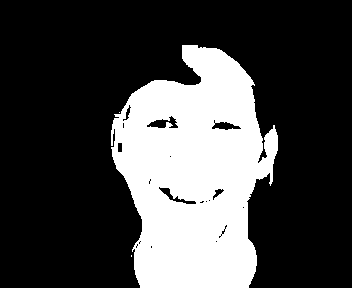
\includegraphics[width=\textwidth]{images/results/base/im00060_y.png}
     \end{subfigure}
    \hfill
     \begin{subfigure}[b]{0.18\textwidth}
         \centering
         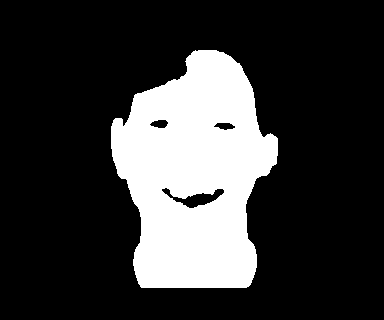
\includegraphics[width=\textwidth]{images/results/base/im00060_skinny_1311.png}
     \end{subfigure}
    \hfill
     \begin{subfigure}[b]{0.18\textwidth}
         \centering
         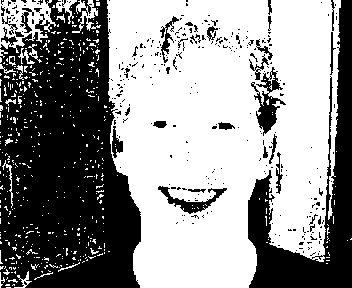
\includegraphics[width=\textwidth]{images/results/base/im00060_bayes_base_ecu.png}
     \end{subfigure}
    \hfill
     \begin{subfigure}[b]{0.18\textwidth}
         \centering
         \includegraphics[width=\textwidth]{images/results/base/im00060_dyc_base_ecu.png}
     \end{subfigure}
     % ROW 2
     \begin{subfigure}[b]{0.18\textwidth}
         \centering
         \includegraphics[width=\textwidth]{images/results/base/im00077_x.jpg}
     \end{subfigure}
     \hfill
     \begin{subfigure}[b]{0.18\textwidth}
         \centering
         \includegraphics[width=\textwidth]{images/results/base/im00077_y.png}
     \end{subfigure}
    \hfill
     \begin{subfigure}[b]{0.18\textwidth}
         \centering
         \includegraphics[width=\textwidth]{images/results/base/im00077_skinny_1272.png}
     \end{subfigure}
    \hfill
     \begin{subfigure}[b]{0.18\textwidth}
         \centering
         \includegraphics[width=\textwidth]{images/results/base/im00077_bayes.png}
     \end{subfigure}
     \hfill
     \begin{subfigure}[b]{0.18\textwidth}
         \centering
         \includegraphics[width=\textwidth]{images/results/base/im00077_dyc.png}
     \end{subfigure}
     % ROW 3
     \begin{subfigure}[b]{0.18\textwidth}
         \centering
         \includegraphics[width=\textwidth]{images/results/base/hh78.color.d3_x.png}
     \end{subfigure}
     \hfill
     \begin{subfigure}[b]{0.18\textwidth}
         \centering
         \includegraphics[width=\textwidth]{images/results/base/hh78.color.d3_y.png}
     \end{subfigure}
    \hfill
     \begin{subfigure}[b]{0.18\textwidth}
         \centering
         \includegraphics[width=\textwidth]{images/results/base/hh78.color.d3_skinny_5.png}
     \end{subfigure}
    \hfill
     \begin{subfigure}[b]{0.18\textwidth}
         \centering
         \includegraphics[width=\textwidth]{images/results/base/hh78.color.d3_bayes.png}
     \end{subfigure}
    \hfill
     \begin{subfigure}[b]{0.18\textwidth}
         \centering
         \includegraphics[width=\textwidth]{images/results/base/hh78.color.d3_dyc.png}
     \end{subfigure}
     % ROW 4
     \begin{subfigure}[b]{0.18\textwidth}
         \centering
         \includegraphics[width=\textwidth]{images/results/base/lighting_fire_x.png}
     \end{subfigure}
     \hfill
     \begin{subfigure}[b]{0.18\textwidth}
         \centering
         \includegraphics[width=\textwidth]{images/results/base/lighting_fire_y.png}
     \end{subfigure}
    \hfill
     \begin{subfigure}[b]{0.18\textwidth}
         \centering
         \includegraphics[width=\textwidth]{images/results/base/lighting_fire_skinny_115.png}
     \end{subfigure}
    \hfill
     \begin{subfigure}[b]{0.18\textwidth}
         \centering
         \includegraphics[width=\textwidth]{images/results/base/lighting_fire_bayes.png}
     \end{subfigure}
    \hfill
     \begin{subfigure}[b]{0.18\textwidth}
         \centering
         \includegraphics[width=\textwidth]{images/results/base/lighting_fire_dyc.png}
     \end{subfigure}
     % ROW 5
     \begin{subfigure}[b]{0.18\textwidth}
         \centering
         \includegraphics[width=\textwidth]{images/results/base/1_A_hgr2A2_id01_1_x.jpg}
     \end{subfigure}
     \hfill
     \begin{subfigure}[b]{0.18\textwidth}
         \centering
         \includegraphics[width=\textwidth]{images/results/base/1_A_hgr2A2_id01_1_y.png}
     \end{subfigure}
    \hfill
     \begin{subfigure}[b]{0.18\textwidth}
         \centering
         \includegraphics[width=\textwidth]{images/results/base/1_A_hgr2A2_id01_1_skinny_8.png}
     \end{subfigure}
    \hfill
     \begin{subfigure}[b]{0.18\textwidth}
         \centering
         \includegraphics[width=\textwidth]{images/results/base/1_A_hgr2A2_id01_1_bayes.png}
     \end{subfigure}
    \hfill
     \begin{subfigure}[b]{0.18\textwidth}
         \centering
         \includegraphics[width=\textwidth]{images/results/base/1_A_hgr2A2_id01_1_dyc.png}
     \end{subfigure}
     % ROW 6
     \begin{subfigure}[b]{0.18\textwidth}
         \centering
         \includegraphics[width=\textwidth]{images/results/base/greenland.205.color.d3_x.png}
         \caption{}
     \end{subfigure}
     \hfill
     \begin{subfigure}[b]{0.18\textwidth}
         \centering
         \includegraphics[width=\textwidth]{images/results/base/greenland.205.color.d3_y.png}
         \caption{}
     \end{subfigure}
    \hfill
     \begin{subfigure}[b]{0.18\textwidth}
         \centering
         \includegraphics[width=\textwidth]{images/results/base/greenland.205.color.d3_skinny.png}
         \caption{}
     \end{subfigure}
    \hfill
     \begin{subfigure}[b]{0.18\textwidth}
         \centering
         \includegraphics[width=\textwidth]{images/results/base/greenland.205.color.d3_bayes.png}
         \caption{}
     \end{subfigure}
     \hfill
     \begin{subfigure}[b]{0.18\textwidth}
         \centering
         \includegraphics[width=\textwidth]{images/results/base/greenland.205.color.d3_dyc.png}
         \caption{}
     \end{subfigure}
        \caption{Skin detection results in datasets single evaluation: (a) the input image; (b) the ground truth; (c) Tarasiewicz \textit{et al.} 2020~\cite{tarasiewicz2020skinny}; (d) Acharjee~\cite{acharjee2018skin}; (e) Brancati \textit{et al.} 2017~\cite{brancati2017human}.\\
        In all the following results, Tarasiewicz \textit{et al.} 2020~\cite{tarasiewicz2020skinny} predictions have different dimensions than other images due to the network preprocessing.}
        \label{fig:base-normal-samples}
\end{figure}


\FloatBarrier
%%%%%%%%%%%%%%%%%%%%%%%%%%%%%%%%%%%%%%%%%%%%%%%%%%%%%%%%%%%%%%%%%%%%%%%%
\section{Performance across databases}
%%%%%%%%%%%%%%%%%%%%%%%%%%%%%%%%%%%%%%%%%%%%%%%%%%%%%%%%%%%%%%%%%%%%%%%%

In the cross evaluation of the datasets (present at \autoref{tab:cross-normal}), the deep learning approach still dominates, but there are some interesting exceptions.
In fact, using HGR as the training set and predicting over Schmugge, Acharjee 2018~\cite{acharjee2018skin} outperforms Tarasiewicz \textit{et al.} 2020~\cite{tarasiewicz2020skinny}, especially in the F\textsubscript{1} score.
This means that, while the statistical method generally performs better than Tarasiewicz \textit{et al.} 2020~\cite{tarasiewicz2020skinny}, it also includes a lot of False Positives, as the F\textsubscript{1}-IoU and the D\textsubscript{prs} metrics indicate.
The latter is particularly bad in both cases, evidencing a big distance between the ideal ground truths and the predictions.
In the case where ECU is used to train and Schmugge to predict, and in the opposite case, Tarasiewicz \textit{et al.} 2020~\cite{tarasiewicz2020skinny} beats the statistical method discretely.
In the latter case, the U-Net describes a slightly worse F\textsubscript{1}-IoU, suggesting the presence of False Positives and False Negatives.
Tarasiewicz \textit{et al.} 2020~\cite{tarasiewicz2020skinny} outperforms the other machine learning approach by far in the remaining cases.
The U-Net exceeds an F\textsubscript{1} score of 80 in the case of Schmugge as the training set and HGR as the prediction set despite the size of the training set, which is not huge.

\begin{table}[ht]
    \centering
    \resizebox{\columnwidth}{!}{
        \begin{tabular}{clcccccc}
        \toprule
        \multicolumn{1}{c}{} & \multicolumn{1}{c}{Training} 
        & \multicolumn{2}{c}{ECU} & \multicolumn{2}{c}{HGR} & \multicolumn{2}{c}{SCHMUGGE} \\\multicolumn{1}{c}{} & \multicolumn{1}{c}{Testing}  & \multicolumn{1}{c}{HGR}  & \multicolumn{1}{c}{SCHMUGGE}  & \multicolumn{1}{c}{ECU}  & \multicolumn{1}{c}{SCHMUGGE}  & \multicolumn{1}{c}{ECU}  & \multicolumn{1}{c}{HGR} \\
        \midrule\multirow{2}{*}{{$F_1$ $\uparrow$}}& Taras. \textit{et al.}~\cite{tarasiewicz2020skinny}\rule{0pt}{14pt} & \monosp{\monobold{0.9308 \pm 0.11}} & \monosp{\monobold{0.4625 \pm 0.41}} & \monosp{\monobold{0.7252 \pm 0.20}} & \monosp{0.2918 \pm 0.31} & \monosp{\monobold{0.6133 \pm 0.21}} & \monosp{\monobold{0.8106 \pm 0.19}}\\& Acharjee~\cite{acharjee2018skin} & \monosp{0.5577 \pm 0.29} & \monosp{0.3319 \pm 0.28} & \monosp{0.4279 \pm 0.19} & \monosp{\monobold{0.4000 \pm 0.32}} & \monosp{0.4638 \pm 0.23} & \monosp{0.5060 \pm 0.25}\\\multirow{2}{*}{{$IoU$ $\uparrow$}}& Taras. \textit{et al.}~\cite{tarasiewicz2020skinny}\rule{0pt}{14pt} & \monosp{\monobold{0.8851 \pm 0.15}} & \monosp{\monobold{0.3986 \pm 0.37}} & \monosp{\monobold{0.6038 \pm 0.22}} & \monosp{0.2168 \pm 0.25} & \monosp{\monobold{0.4754 \pm 0.22}} & \monosp{\monobold{0.7191 \pm 0.23}}\\& Acharjee~\cite{acharjee2018skin} & \monosp{0.4393 \pm 0.27} & \monosp{0.2346 \pm 0.21} & \monosp{0.2929 \pm 0.17} & \monosp{\monobold{0.2981 \pm 0.24}} & \monosp{0.3318 \pm 0.20} & \monosp{0.3752 \pm 0.22}\\\multirow{2}{*}{{$D_{prs}$ $\downarrow$}}& Taras. \textit{et al.}~\cite{tarasiewicz2020skinny}\rule{0pt}{14pt} & \monosp{\monobold{0.1098 \pm 0.15}} & \monosp{\monobold{0.7570 \pm 0.56}} & \monosp{\monobold{0.3913 \pm 0.26}} & \monosp{\monobold{0.9695 \pm 0.44}} & \monosp{\monobold{0.5537 \pm 0.27}} & \monosp{\monobold{0.2846 \pm 0.27}}\\& Acharjee~\cite{acharjee2018skin} & \monosp{0.5701 \pm 0.29} & \monosp{1.0477 \pm 0.35} & \monosp{0.8830 \pm 0.23} & \monosp{1.0219 \pm 0.42} & \monosp{0.7542 \pm 0.30} & \monosp{0.6523 \pm 0.27}\\\multirow{2}{*}{{$F_1 - IoU$ $\downarrow$}}& Taras. \textit{et al.}~\cite{tarasiewicz2020skinny}\rule{0pt}{14pt} & \monosp{\monobold{0.0457}} & \monosp{\monobold{0.0639}} & \monosp{\monobold{0.1214}} & \monosp{\monobold{0.0750}} & \monosp{0.1379} & \monosp{\monobold{0.0915}}\\& Acharjee~\cite{acharjee2018skin} & \monosp{0.1184} & \monosp{0.0973} & \monosp{0.1350} & \monosp{0.1019} & \monosp{\monobold{0.1320}} & \monosp{0.1308}\\
        \bottomrule
        \end{tabular}}
    \caption{Cross evaluation on datasets.\\
        For each dataset: methods are trained on the training set and then predictions are performed on all the images of every other datasets.\\
        For example, with ECU as the training dataset and HGR as the testing dataset, it means that a method is trained using the training set of ECU, and then tested on all the HGR dataset.}
    \label{tab:cross-normal}
\end{table}

Some interesting instances are shown in \autoref{fig:cross-normal-samples}.
The expression \q{HGR on ECU} describes the situation in which the evaluation is performed by using HGR as the training set and ECU as the test set. In cross evaluations, this type of expression is going to be used a lot to avoid text redundancy.
The first row (HGR on ECU) shows a really poor classification by the statistical approach.
In the second row (ECU on Schmugge) it can be noticed how Acharjee 2018~\cite{acharjee2018skin} tends to exaggerate at classifying skin pixels in some cases, confirming the above intuitions on the statistical method having a lot of False Positives.
The third row (ECU on Schmugge) describes a tragic classification by Tarasiewicz \textit{et al.} 2020~\cite{tarasiewicz2020skinny}, that might be caused by the presence of tricky lighting conditions and shadows on the skin regions.
The statistical approach performs badly too, but still has a lot better classification.
In this case, the ground truth shows how incorporating the ambiguous regions provided by the Schmugge database makes the skin regions quite pixels-hungry on the border with non-skin regions.
The fourth image (Schmugge on ECU) represents a bad classification in both approaches, where there is especially an outstanding number of False Positives.
The next-to-last image (HGR on Schmugge) is part of the datasets combination in which Acharjee 2018~\cite{acharjee2018skin} outperforms the deep learning one.
The statistical method reports a lot of False Positives, but also a lot of True Positives, which Tarasiewicz \textit{et al.} 2020~\cite{tarasiewicz2020skinny} struggles to identify.
The last picture (HGR on Schmugge) is also part of the same datasets combination and describes a similar situation: the U-Net fails at labeling several skin pixels, especially on very lit regions, while the statistical method overdoes it.
This image represents the high complexity and diversity of the Schmugge content.

\begin{figure}[h]
     \centering
     
     \resizebox{0.8\textwidth}{0.17\textheight}{
     % ROW 1
     \begin{subfigure}[b]{0.23\textwidth}
         \centering
         \includegraphics[width=\textwidth]{images/results/cross/5_A_hgr2B_id10_1_ecu_hgr_x.jpg}
     \end{subfigure}
     \hfill
     \begin{subfigure}[b]{0.23\textwidth}
         \centering
         \includegraphics[width=\textwidth]{images/results/cross/5_A_hgr2B_id10_1_ecu_hgr_y.png}
     \end{subfigure}
    \hfill
     \begin{subfigure}[b]{0.23\textwidth}
         \centering
         \includegraphics[width=\textwidth]{images/results/cross/5_A_hgr2B_id10_1_ecu_hgr_skinny_123.png}
     \end{subfigure}
    \hfill
     \begin{subfigure}[b]{0.23\textwidth}
         \centering
         \includegraphics[width=\textwidth]{images/results/cross/5_A_hgr2B_id10_1_ecu_hgr_bayes.png}
     \end{subfigure}}
     
     \resizebox{0.8\textwidth}{0.17\textheight}{
     % ROW 2
     \begin{subfigure}[b]{0.23\textwidth}
         \centering
         \includegraphics[width=\textwidth]{images/results/cross/aa46_1.color.d3_ecu_sch_x.png}
     \end{subfigure}
     \hfill
     \begin{subfigure}[b]{0.23\textwidth}
         \centering
         \includegraphics[width=\textwidth]{images/results/cross/aa46_1.color.d3_ecu_sch_y.png}
     \end{subfigure}
    \hfill
     \begin{subfigure}[b]{0.23\textwidth}
         \centering
         \includegraphics[width=\textwidth]{images/results/cross/aa46_1.color.d3_ecu_sch_skinny283.png}
     \end{subfigure}
    \hfill
     \begin{subfigure}[b]{0.23\textwidth}
         \centering
         \includegraphics[width=\textwidth]{images/results/cross/aa46_1.color.d3_ecu_sch_bayes.png}
     \end{subfigure}}
    
     \resizebox{0.8\textwidth}{0.18\textheight}{
     % ROW 3
     \begin{subfigure}[b]{0.23\textwidth}
         \centering
         \includegraphics[width=\textwidth]{images/results/cross/att-massu.jpg_ecu_sch_x.png}
     \end{subfigure}
     \hfill
     \begin{subfigure}[b]{0.23\textwidth}
         \centering
         \includegraphics[width=\textwidth]{images/results/cross/att-massu_ecu_sch_y.png}
     \end{subfigure}
    \hfill
     \begin{subfigure}[b]{0.23\textwidth}
         \centering
         \includegraphics[width=\textwidth]{images/results/cross/att-massu.jpg_ecu_sch_skinny_157.png}
     \end{subfigure}
    \hfill
     \begin{subfigure}[b]{0.23\textwidth}
         \centering
         \includegraphics[width=\textwidth]{images/results/cross/att-massu_ecu_sch_bayes.png}
     \end{subfigure}}
     
     \resizebox{0.8\textwidth}{0.08\textheight}{
     % ROW 4
     \begin{subfigure}[b]{0.23\textwidth}
         \centering
         \includegraphics[width=\textwidth]{images/results/cross/im00593_sch_ecu_x.jpg}
     \end{subfigure}
     \hfill
     \begin{subfigure}[b]{0.23\textwidth}
         \centering
         \includegraphics[width=\textwidth]{images/results/cross/im00593_sch_ecu_y.png}
     \end{subfigure}
    \hfill
     \begin{subfigure}[b]{0.23\textwidth}
         \centering
         \includegraphics[width=\textwidth]{images/results/cross/im00593_sch_ecu_skinny_424.png}
     \end{subfigure}
    \hfill
     \begin{subfigure}[b]{0.23\textwidth}
         \centering
         \includegraphics[width=\textwidth]{images/results/cross/im00593_sch_ecu_bayes.png}
     \end{subfigure}}
     
     \resizebox{0.8\textwidth}{0.2\textheight}{
     % ROW 5
     \begin{subfigure}[b]{0.23\textwidth}
         \centering
         \includegraphics[width=\textwidth]{images/results/cross/linda_rgb_hgr_sch_x.png}
     \end{subfigure}
     \hfill
     \begin{subfigure}[b]{0.23\textwidth}
         \centering
         \includegraphics[width=\textwidth]{images/results/cross/linda_rgb_hgr_sch_y.png}
     \end{subfigure}
    \hfill
     \begin{subfigure}[b]{0.23\textwidth}
         \centering
         \includegraphics[width=\textwidth]{images/results/cross/linda_rgb_hgr_sch_skinny120.png}
     \end{subfigure}
    \hfill
     \begin{subfigure}[b]{0.23\textwidth}
         \centering
         \includegraphics[width=\textwidth]{images/results/cross/linda_rgb_hgr_sch_bayes.png}
     \end{subfigure}}
     
     \resizebox{0.8\textwidth}{0.10\textheight}{
     % ROW 6
     \begin{subfigure}[b]{0.23\textwidth}
         \centering
         \includegraphics[width=\textwidth]{images/results/cross/w-020-7.color.d3_hgr_sch_x.png}
         \caption{}
     \end{subfigure}
     \hfill
     \begin{subfigure}[b]{0.23\textwidth}
         \centering
         \includegraphics[width=\textwidth]{images/results/cross/w-020-7.color.d3_hgr_sch_y.png}
         \caption{}
     \end{subfigure}
    \hfill
     \begin{subfigure}[b]{0.23\textwidth}
         \centering
         \includegraphics[width=\textwidth]{images/results/cross/w-020-7.color.d3_hgr_sch_skinny_426.png}
         \caption{}
     \end{subfigure}
    \hfill
     \hfill
     \begin{subfigure}[b]{0.23\textwidth}
         \centering
         \includegraphics[width=\textwidth]{images/results/cross/w-020-7.color.d3_hgr_sch_bayes.png}
         \caption{}
     \end{subfigure}}
\caption{Skin detection results in datasets cross evaluation: (a) the input image; (b) the ground truth; (c) Tarasiewicz \textit{et al.} 2020~\cite{tarasiewicz2020skinny}; (d) Acharjee~\cite{acharjee2018skin}}
\label{fig:cross-normal-samples}
\end{figure}%


\FloatBarrier
%%%%%%%%%%%%%%%%%%%%%%%%%%%%%%%%%%%%%%%%%%%%%%%%%%%%%%%%%%%%%%%%%%%%%%%%
\section{Performance on single Skin tones}
%%%%%%%%%%%%%%%%%%%%%%%%%%%%%%%%%%%%%%%%%%%%%%%%%%%%%%%%%%%%%%%%%%%%%%%%

In the single evaluation of the skin tones sub-datasets (present at \autoref{tab:base-skin-tones}), the U-Net outperforms the competitors in all cases, and the thresholding approach comes last in all cases.
The learning approaches describe a very low standard deviation on the darker skin tones, indicating that the diversity of the images might not be very high.
Tarasiewicz \textit{et al.} 2020~\cite{tarasiewicz2020skinny} reports outstanding scores, having almost ground truth-like predictions, as described by the D\textsubscript{prs} measure.
Brancati \textit{et al.} 2017~\cite{brancati2017human} instead describes horrible results, which may indicate that the skin clustering rules are leaving out the darker skin pixels.
The machine learning methods have the highest difficulty at classifying the medium skin tones, which pictures include a lot of difficult scenarios, such as clay terrains that are skin-like colored.
Despite the troubles, all the approaches report generally good scores on both medium and light skin tones, especially the machine learning methods.

\begin{table}[ht]
    \centering
    \resizebox{\columnwidth}{!}{
    \begin{tabular}{clccc}
    \toprule
    & Method\textbackslash Database & DARK & MEDIUM & LIGHT \\
    \midrule
    %
    %
    \multirow{3}{*}{{$F_1 \uparrow$}}
        & Tarasiewicz \textit{et al.}~\cite{tarasiewicz2020skinny}
        & $\pmb{0.9529 \pm 0.00}$ & $\pmb{0.9260 \pm 0.15}$ & $\pmb{0.9387 \pm 0.12}$ \\
        %
        & Acharjee~\cite{acharjee2018skin}
        & $\underline{0.8123 \pm 0.02}$ & $\underline{0.7634 \pm 0.19}$ & $\underline{0.8001 \pm 0.15}$ \\
        %
        & Brancati \textit{et al.}~\cite{brancati2017human}
        & $0.2620 \pm 0.14$ & $0.6316 \pm 0.20$ & $0.6705 \pm 0.14$ \\[5pt]
        %
        %
    \multirow{3}{*}{{$IoU \uparrow$}}
        & Tarasiewicz \textit{et al.}~\cite{tarasiewicz2020skinny}
        & $\pmb{0.9100 \pm 0.01}$ & $\pmb{0.8883 \pm 0.18}$ & $\pmb{0.9006 \pm 0.14}$ \\
        %
        & Acharjee~\cite{acharjee2018skin}
        & $\underline{0.6844 \pm 0.03}$ & $\underline{0.6432 \pm 0.17}$ & $\underline{0.6870 \pm 0.16}$ \\
        %
        & Brancati \textit{et al.}~\cite{brancati2017human}
        & $0.1587 \pm 0.10$ & $0.4889 \pm 0.19$ & $0.5190 \pm 0.14$ \\[5pt]
        %
        %
    \multirow{3}{*}{{$D_{prs} \downarrow$}}
        & Tarasiewicz \textit{et al.}~\cite{tarasiewicz2020skinny}
        & $\pmb{0.0720 \pm 0.01}$ & $\pmb{0.1078 \pm 0.21}$ & $\pmb{0.0926 \pm 0.15}$ \\
        %
        & Acharjee~\cite{acharjee2018skin}
        & $\underline{0.3406 \pm 0.05}$ & $\underline{0.3452 \pm 0.23}$ & $\underline{0.3054 \pm 0.20}$ \\
        %
        & Brancati \textit{et al.}~\cite{brancati2017human}
        & $0.8548 \pm 0.12 $ & $0.5155 \pm 0.24$ & $0.4787 \pm 0.17$\\
        %
        %
    \bottomrule
    \end{tabular}}
    \caption{Single evaluation on skin tones.\\
     For each dataset: methods are eventually trained on the training set, in the case of trainable methods, and then predictions are performed on the test set.\\
     For example, with DARK as the dataset, it means that a method is trained using the training set of DARK, if the method is trainable, and then tested on the test set of DARK.
    }
    \label{tab:base-skin-tones}
\end{table}

Some interesting instances can be seen in \autoref{fig:base-skintones-samples}.
The first two rows depict darker skin tones.
In both examples, it is possible to notice a pattern in the classification of each approach: Tarasiewicz \textit{et al.} 2020~\cite{tarasiewicz2020skinny} produces almost ground truth-like predictions; the statistical method tends to exaggerate on classifying skin pixels, but has an excellent number of True Positives; Brancati \textit{et al.} 2017~\cite{brancati2017human} seems to fail at classifying the darkest skin tones.
The next two rows represent medium skin tones.
The following row reports similar results to the dark skin tones rows, but in this case the thresholding approach has good results.
It is noticeable that, while the statistical method tends to include many False Positives, the thresholding one is a lot more conservative, marking only the inner regions of the face, which are sufficient for describing the face shape.
The last row of medium skin tones represents a tricky background with a clay terrain.
Tarasiewicz \textit{et al.} 2020~\cite{tarasiewicz2020skinny} produces a very good prediction, while the other approaches include many False Positives.
Acharjee 2018~\cite{acharjee2018skin} reports a tremendous number of False Positives, while Brancati \textit{et al.} 2017~\cite{brancati2017human} is deceived by the clay terrain and ruins its otherwise excellent classification.
The last two rows feature people with light skin tones.
In the starting row, the U-Net and the rule-based approaches have very good predictions, with Tarasiewicz \textit{et al.} 2020~\cite{tarasiewicz2020skinny} incorporating more False Positives, and Brancati \textit{et al.} 2017~\cite{brancati2017human} including more False Negatives.
The statistical approach reports once again a huge number of False Positives.
The last row depicts good results on all methods and shows some limitations that Brancati \textit{et al.} 2017~\cite{brancati2017human} seems to have on tricky lighting conditions.

\begin{figure}[h]
     \centering
     % ROW 1
     \begin{subfigure}[b]{0.18\textwidth}
         \centering
         \includegraphics[width=\textwidth]{images/results/base_st/dd109.color.d3_x.png}
     \end{subfigure}
     \hfill
     \begin{subfigure}[b]{0.18\textwidth}
         \centering
         \includegraphics[width=\textwidth]{images/results/base_st/dd109.color.d3_y.png}
     \end{subfigure}
    \hfill
     \begin{subfigure}[b]{0.18\textwidth}
         \centering
         \includegraphics[width=\textwidth]{images/results/base_st/dd109.color.d3_skinny_4.png}
     \end{subfigure}
    \hfill
     \begin{subfigure}[b]{0.18\textwidth}
         \centering
         \includegraphics[width=\textwidth]{images/results/base_st/dd109.color.d3_bayes.png}
     \end{subfigure}
    \hfill
     \begin{subfigure}[b]{0.18\textwidth}
         \centering
         \includegraphics[width=\textwidth]{images/results/base_st/dd109.color.d3_dyc.png}
     \end{subfigure}
     % ROW 2
     \begin{subfigure}[b]{0.18\textwidth}
         \centering
         \includegraphics[width=\textwidth]{images/results/base_st/dd110.color.d3_x.png}
     \end{subfigure}
     \hfill
     \begin{subfigure}[b]{0.18\textwidth}
         \centering
         \includegraphics[width=\textwidth]{images/results/base_st/dd110.color.d3_y.png}
     \end{subfigure}
    \hfill
     \begin{subfigure}[b]{0.18\textwidth}
         \centering
         \includegraphics[width=\textwidth]{images/results/base_st/dd110.color.d3_skinny_2.png}
     \end{subfigure}
    \hfill
     \begin{subfigure}[b]{0.18\textwidth}
         \centering
         \includegraphics[width=\textwidth]{images/results/base_st/dd110.color.d3_bayes.png}
     \end{subfigure}
     \hfill
     \begin{subfigure}[b]{0.18\textwidth}
         \centering
         \includegraphics[width=\textwidth]{images/results/base_st/dd110.color.d3_dyc.png}
     \end{subfigure}
     % ROW 3
     \begin{subfigure}[b]{0.18\textwidth}
         \centering
         \includegraphics[width=\textwidth]{images/results/base_st/dd121.color.d3_x.png}
     \end{subfigure}
     \hfill
     \begin{subfigure}[b]{0.18\textwidth}
         \centering
         \includegraphics[width=\textwidth]{images/results/base_st/dd121.color.d3_y.png}
     \end{subfigure}
    \hfill
     \begin{subfigure}[b]{0.18\textwidth}
         \centering
         \includegraphics[width=\textwidth]{images/results/base_st/dd121.color.d3_skinny_13.png}
     \end{subfigure}
    \hfill
     \begin{subfigure}[b]{0.18\textwidth}
         \centering
         \includegraphics[width=\textwidth]{images/results/base_st/dd121.color.d3_bayes.png}
     \end{subfigure}
    \hfill
     \begin{subfigure}[b]{0.18\textwidth}
         \centering
         \includegraphics[width=\textwidth]{images/results/base_st/dd121.color.d3_dyc.png}
     \end{subfigure}
     % ROW 4
     \begin{subfigure}[b]{0.18\textwidth}
         \centering
         \includegraphics[width=\textwidth]{images/results/base_st/ivan1_x.png}
     \end{subfigure}
     \hfill
     \begin{subfigure}[b]{0.18\textwidth}
         \centering
         \includegraphics[width=\textwidth]{images/results/base_st/ivan1_y.png}
     \end{subfigure}
    \hfill
     \begin{subfigure}[b]{0.18\textwidth}
         \centering
         \includegraphics[width=\textwidth]{images/results/base_st/ivan1_skinny_2.png}
     \end{subfigure}
    \hfill
     \begin{subfigure}[b]{0.18\textwidth}
         \centering
         \includegraphics[width=\textwidth]{images/results/base_st/ivan1_bayes.png}
     \end{subfigure}
    \hfill
     \begin{subfigure}[b]{0.18\textwidth}
         \centering
         \includegraphics[width=\textwidth]{images/results/base_st/ivan1_dyc.png}
     \end{subfigure}
     % ROW 5
     \begin{subfigure}[b]{0.18\textwidth}
         \centering
         \includegraphics[width=\textwidth]{images/results/base_st/wd2002-sue-shaded-hat_x.png}
     \end{subfigure}
     \hfill
     \begin{subfigure}[b]{0.18\textwidth}
         \centering
         \includegraphics[width=\textwidth]{images/results/base_st/wd2002-sue-shaded-hat_y.png}
     \end{subfigure}
    \hfill
     \begin{subfigure}[b]{0.18\textwidth}
         \centering
         \includegraphics[width=\textwidth]{images/results/base_st/wd2002-sue-shaded-hat_skinny_22.png}
     \end{subfigure}
    \hfill
     \begin{subfigure}[b]{0.18\textwidth}
         \centering
         \includegraphics[width=\textwidth]{images/results/base_st/wd2002-sue-shaded-hat_bayes.png}
     \end{subfigure}
    \hfill
     \begin{subfigure}[b]{0.18\textwidth}
         \centering
         \includegraphics[width=\textwidth]{images/results/base_st/wd2002-sue-shaded-hat_dyc.png}
     \end{subfigure}
     % ROW 6
     \begin{subfigure}[b]{0.18\textwidth}
         \centering
         \includegraphics[width=\textwidth]{images/results/base_st/m-022-5.color.d3_x.png}
         \caption{}
     \end{subfigure}
     \hfill
     \begin{subfigure}[b]{0.18\textwidth}
         \centering
         \includegraphics[width=\textwidth]{images/results/base_st/m-022-5.color.d3_y.png}
         \caption{}
     \end{subfigure}
    \hfill
     \begin{subfigure}[b]{0.18\textwidth}
         \centering
         \includegraphics[width=\textwidth]{images/results/base_st/m-022-5.color.d3_skinny_25.png}
         \caption{}
     \end{subfigure}
    \hfill
     \begin{subfigure}[b]{0.18\textwidth}
         \centering
         \includegraphics[width=\textwidth]{images/results/base_st/m-022-5.color.d3_bayes.png}
         \caption{}
     \end{subfigure}
     \hfill
     \begin{subfigure}[b]{0.18\textwidth}
         \centering
         \includegraphics[width=\textwidth]{images/results/base_st/m-022-5.color.d3_dyc.png}
         \caption{}
     \end{subfigure}
        \caption{Skin detection results in skin tones single evaluation: (a) the input image; (b) the ground truth; (c) Tarasiewicz \textit{et al.} 2020~\cite{tarasiewicz2020skinny}; (d) Acharjee~\cite{acharjee2018skin}; (e) Brancati \textit{et al.} 2017~\cite{brancati2017human}.}
        \label{fig:base-skintones-samples}
\end{figure}


\FloatBarrier
%%%%%%%%%%%%%%%%%%%%%%%%%%%%%%%%%%%%%%%%%%%%%%%%%%%%%%%%%%%%%%%%%%%%%%%%
\section{Performance across Skin tones}
%%%%%%%%%%%%%%%%%%%%%%%%%%%%%%%%%%%%%%%%%%%%%%%%%%%%%%%%%%%%%%%%%%%%%%%%

The cross evaluation of the skin tones sub-datasets, \autoref{tab:cross-skin-tones}), describes some interesting situations.
As usual, the U-Net outperforms the other machine learning approach in most situations, but it is outperformed a pair of times.
In fact, using the darker skin tones as training and predicting on the medium skin tones makes Acharjee 2018~\cite{acharjee2018skin} the seemingly better classifier.
It describes best scores in all metrics but the difference between F\textsubscript{1} and D\textsubscript{prs}, with also a lower population standard deviation.
The dark sub-dataset was the smallest one and therefore has been data-augmented.
However, the augmentation has been performed with light transformations that do not detach from the original images too much.
Hence, these scores may indicate that Acharjee 2018~\cite{acharjee2018skin} performs better with a smaller training set.
Anyway, Tarasiewicz \textit{et al.} 2020~\cite{tarasiewicz2020skinny} describes only slightly worse results and reports good classifications in this scenario too.
The higher difference between F\textsubscript{1} and D\textsubscript{prs} may indicate the usual greedy that the statistical method demonstrates on False Positives.
The dark on light case is particularly interesting because the statistical approach wins on the F\textsubscript{1}-Score, but is outperformed in all the others.
Winning on the F\textsubscript{1}-Score and losing on the IoU means that the statistical approach picks more True Positives than the deep learning one.
Tarasiewicz \textit{et al.} 2020~\cite{tarasiewicz2020skinny} also describes more unstable results as the population standard deviation is higher.
The F\textsubscript{1} and IoU scores are relatively close between the approaches, but the D\textsubscript{prs} is far better with Tarasiewicz \textit{et al.} 2020~\cite{tarasiewicz2020skinny}.
This behavior may suggest, along with the F\textsubscript{1} and IoU considerations, and the fact that their difference is higher on the statistical method, the presence of many False Positives and/or False Negatives, which however seems unlikely given the previous observations, on the statistical method predictions.
All the other situations have the U-Net winning on the scores by a great degree.
In the medium on dark situation, Acharjee 2018~\cite{acharjee2018skin} describes a very high D\textsubscript{prs}, even higher than the light on dark case, where the F\textsubscript{1} and IoU scores are worse.
This is a clear indicator that the Specificity is driving the prediction away from the ideal ground truth, so it may be an indicator of a very small number of True Negatives.
Tarasiewicz \textit{et al.} 2020~\cite{tarasiewicz2020skinny} presents the highest score in the light on medium case, which may be a signal of the need of having bigger training data, but on the other hand, it performs far worse on the light on dark case, indicating that a bigger training data might not be sufficient.
In fact, the U-Net describes the best average score by training on the medium skin tones, which represent a smaller dataset than the lighter skin tones, but a midpoint between the colors of darker and lighter skin tones.
This may be a representation of how the Neural Network adapts and learns to classify new skin tones.

Some interesting instances are reported in \autoref{fig:cross-skintones-samples}.
The first two rows represent dark on medium cases.
The results seem to confirm the earlier guesses on the statistical method incorporating a lot of False Positives.
Tarasiewicz \textit{et al.} 2020~\cite{tarasiewicz2020skinny} depicts a terrible classification, with a lot of False Positives and False Negatives.
In the second row, the tricky lighting causes troubles to the U-Net, which provides another terrible prediction, while the statistical method has a far better prediction, despite including a lot of False Positives too.
The third row and the fourth row represent dark on light situations.
Tarasiewicz \textit{et al.} 2020~\cite{tarasiewicz2020skinny} produces an awful prediction even in these cases, featuring particularly a lot of False Negatives.
Acharjee 2018~\cite{acharjee2018skin} does the opposite and once again exaggerates as usual with the classification of skin pixels.
The original images of these two rows are also featured in \autoref{fig:cross-normal-samples}, where they reported similar issues, so it seems that both approaches struggle to adapt to skin pixels different from the ones of the training set in these types of images.
The smallest image depicts a quite extreme and unnatural level of lighting, hence the issues are easily justifiable.
The other image seems to depict a more natural skin tone, but it must be taken into account that it may still be far from the skin tones of the training set, which may be too light or dark. 
The fifth row features a medium on dark case, where the hypothesis of having very few True Negatives, driving the D\textsubscript{prs} measure high, seems confirmed.
Tarasiewicz \textit{et al.} 2020~\cite{tarasiewicz2020skinny} on the other hand performs a quite good classification, marking almost correctly most of the skin regions.
The last row represents a light on dark case on the same original picture of the previous row, with the purpose of a quick comparison.
In this case, the statistical approach does a much better job, especially at predicting non-skin pixels, which may indicate that the light sub-dataset contains more images featuring sky and water labeled as non-skin pixels.
Tarasiewicz \textit{et al.} 2020~\cite{tarasiewicz2020skinny} performs quite similarly to the previous instance.

\begin{table}[ht]
    \centering
    \resizebox{\columnwidth}{!}{
    \begin{tabular}{clcccccc}
    \toprule
    \multicolumn{1}{c}{} & \multicolumn{1}{c}{Training} 
    & \multicolumn{2}{c}{DARK} & \multicolumn{2}{c}{MEDIUM} & \multicolumn{2}{c}{LIGHT} \\\multicolumn{1}{c}{} & \multicolumn{1}{c}{Testing}  & \multicolumn{1}{c}{MEDIUM}  & \multicolumn{1}{c}{LIGHT}  & \multicolumn{1}{c}{DARK}  & \multicolumn{1}{c}{LIGHT}  & \multicolumn{1}{c}{DARK}  & \multicolumn{1}{c}{MEDIUM} \\\midrule\multirow{2}{*}{{$F_1$ $\uparrow$}}& Taras. \textit{et al.}~\cite{tarasiewicz2020skinny}\rule{0pt}{14pt} & \monosp{0.7300 \pm 0.25} & \monosp{0.7262 \pm 0.26} & \monosp{\monobold{0.8447 \pm 0.13}} & \monosp{\monobold{0.8904 \pm 0.14}} & \monosp{\monobold{0.7660 \pm 0.17}} & \monosp{\monobold{0.9229 \pm 0.11}}\\& Acharjee~\cite{acharjee2018skin} & \monosp{\monobold{0.7928 \pm 0.11}} & \monosp{\monobold{0.7577 \pm 0.12}} & \monosp{0.5628 \pm 0.14} & \monosp{0.7032 \pm 0.14} & \monosp{0.5293 \pm 0.20} & \monosp{0.7853 \pm 0.11}\\\multirow{2}{*}{{$IoU$ $\uparrow$}}& Taras. \textit{et al.}~\cite{tarasiewicz2020skinny}\rule{0pt}{14pt} & \monosp{0.6279 \pm 0.27} & \monosp{\monobold{0.6276 \pm 0.28}} & \monosp{\monobold{0.7486 \pm 0.15}} & \monosp{\monobold{0.8214 \pm 0.16}} & \monosp{\monobold{0.6496 \pm 0.21}} & \monosp{\monobold{0.8705 \pm 0.13}}\\& Acharjee~\cite{acharjee2018skin} & \monosp{\monobold{0.6668 \pm 0.11}} & \monosp{0.6229 \pm 0.13} & \monosp{0.4042 \pm 0.13} & \monosp{0.5571 \pm 0.14} & \monosp{0.3852 \pm 0.19} & \monosp{0.6574 \pm 0.12}\\\multirow{2}{*}{{$D_{prs}$ $\downarrow$}}& Taras. \textit{et al.}~\cite{tarasiewicz2020skinny}\rule{0pt}{14pt} & \monosp{0.3805 \pm 0.33} & \monosp{\monobold{0.3934 \pm 0.34}} & \monosp{\monobold{0.2326 \pm 0.17}} & \monosp{\monobold{0.1692 \pm 0.18}} & \monosp{\monobold{0.3402 \pm 0.21}} & \monosp{\monobold{0.1192 \pm 0.16}}\\& Acharjee~\cite{acharjee2018skin} & \monosp{\monobold{0.3481 \pm 0.16}} & \monosp{0.4679 \pm 0.18} & \monosp{0.6802 \pm 0.20} & \monosp{0.5376 \pm 0.23} & \monosp{0.6361 \pm 0.22} & \monosp{0.3199 \pm 0.16}\\\multirow{2}{*}{{$F_1 - IoU$ $\downarrow$}}& Taras. \textit{et al.}~\cite{tarasiewicz2020skinny}\rule{0pt}{14pt} & \monosp{\monobold{0.1021}} & \monosp{\monobold{0.0986}} & \monosp{\monobold{0.0961}} & \monosp{\monobold{0.0690}} & \monosp{\monobold{0.1164}} & \monosp{\monobold{0.0524}}\\& Acharjee~\cite{acharjee2018skin} & \monosp{0.1260} & \monosp{0.1348} & \monosp{0.1586} & \monosp{0.1461} & \monosp{0.1441} & \monosp{0.1279}\\
    \bottomrule
    \end{tabular}}
    \caption{Cross evaluation on skin tones.\\
        For each dataset: methods are trained on the training set and then predictions are performed on all the images of every other datasets.\\
        For example, with DARK as the training dataset and LIGHT as the testing dataset, it means that a method is trained using the training set of DARK, and then tested on all the LIGHT dataset.}
    \label{tab:cross-skin-tones}
\end{table}

\begin{figure}[h]
     \centering
     
     \resizebox{0.8\textwidth}{0.17\textheight}{
     % ROW 1
     \begin{subfigure}[b]{0.23\textwidth}
         \centering
         \includegraphics[width=\textwidth]{images/results/cross_st/clay_dark_med_x.png}
     \end{subfigure}
     \hfill
     \begin{subfigure}[b]{0.23\textwidth}
         \centering
         \includegraphics[width=\textwidth]{images/results/cross_st/clay_dark_med_y.png}
     \end{subfigure}
    \hfill
     \begin{subfigure}[b]{0.23\textwidth}
         \centering
         \includegraphics[width=\textwidth]{images/results/cross_st/clay_dark_med_skinny_92.png}
     \end{subfigure}
    \hfill
     \begin{subfigure}[b]{0.23\textwidth}
         \centering
         \includegraphics[width=\textwidth]{images/results/cross_st/clay_dark_med_bayes.png}
     \end{subfigure}}
     
    \resizebox{0.8\textwidth}{0.08\textheight}{
     % ROW 2
     \begin{subfigure}[b]{0.23\textwidth}
         \centering
         \includegraphics[width=\textwidth]{images/results/cross_st/w-020-7.color.d3_dark_med_x.png}
     \end{subfigure}
     \hfill
     \begin{subfigure}[b]{0.23\textwidth}
         \centering
         \includegraphics[width=\textwidth]{images/results/cross_st/w-020-7.color.d3.png}
     \end{subfigure}
    \hfill
     \begin{subfigure}[b]{0.23\textwidth}
         \centering
         \includegraphics[width=\textwidth]{images/results/cross_st/w-020-7.color.d3_dark_med_skinny_57.png}
     \end{subfigure}
    \hfill
     \begin{subfigure}[b]{0.23\textwidth}
         \centering
         \includegraphics[width=\textwidth]{images/results/cross_st/w-020-7.color.d3_dark_med_bayes.png}
     \end{subfigure}}
     
    \resizebox{0.8\textwidth}{0.20\textheight}{
     % ROW 3
     \begin{subfigure}[b]{0.23\textwidth}
         \centering
         \includegraphics[width=\textwidth]{images/results/cross_st/linda_rgb_dark_light_x.png}
     \end{subfigure}
     \hfill
     \begin{subfigure}[b]{0.23\textwidth}
         \centering
         \includegraphics[width=\textwidth]{images/results/cross_st/linda_rgb_dark_light_y.png}
     \end{subfigure}
    \hfill
     \begin{subfigure}[b]{0.23\textwidth}
         \centering
         \includegraphics[width=\textwidth]{images/results/cross_st/linda_rgb_dark_light_skinny_293.png}
     \end{subfigure}
    \hfill
     \begin{subfigure}[b]{0.23\textwidth}
         \centering
         \includegraphics[width=\textwidth]{images/results/cross_st/linda_rgb_dark_light_bayes.png}
     \end{subfigure}}
     
    \resizebox{0.8\textwidth}{0.07\textheight}{
     % ROW 4
     \begin{subfigure}[b]{0.23\textwidth}
         \centering
         \includegraphics[width=\textwidth]{images/results/cross_st/outdoor_cooking_dark_light_x.png}
     \end{subfigure}
     \hfill
     \begin{subfigure}[b]{0.23\textwidth}
         \centering
         \includegraphics[width=\textwidth]{images/results/cross_st/outdoor_cooking_dark_light_y.png}
     \end{subfigure}
    \hfill
     \begin{subfigure}[b]{0.23\textwidth}
         \centering
         \includegraphics[width=\textwidth]{images/results/cross_st/outdoor_cooking_dark_light_skinny_3.png}
     \end{subfigure}
    \hfill
     \begin{subfigure}[b]{0.23\textwidth}
         \centering
         \includegraphics[width=\textwidth]{images/results/cross_st/outdoor_cooking_dark_light_bayes.png}
     \end{subfigure}}
     
     \resizebox{0.8\textwidth}{0.18\textheight}{
     % ROW 5
     \begin{subfigure}[b]{0.23\textwidth}
         \centering
         \includegraphics[width=\textwidth]{images/results/cross_st/mike_med_dark_x.png}
     \end{subfigure}
     \hfill
     \begin{subfigure}[b]{0.23\textwidth}
         \centering
         \includegraphics[width=\textwidth]{images/results/cross_st/mike_med_dark_y.png}
     \end{subfigure}
    \hfill
     \begin{subfigure}[b]{0.23\textwidth}
         \centering
         \includegraphics[width=\textwidth]{images/results/cross_st/mike_med_dark_skinny_19.png}
     \end{subfigure}
    \hfill
     \begin{subfigure}[b]{0.23\textwidth}
         \centering
         \includegraphics[width=\textwidth]{images/results/cross_st/mike_med_dark_bayes.png}
     \end{subfigure}}
     
     \resizebox{0.8\textwidth}{0.20\textheight}{
     % ROW 6
     \begin{subfigure}[b]{0.23\textwidth}
         \centering
         \includegraphics[width=\textwidth]{images/results/cross_st/mike_light_dark_x.png}
         \caption{}
     \end{subfigure}
     \hfill
     \begin{subfigure}[b]{0.23\textwidth}
         \centering
         \includegraphics[width=\textwidth]{images/results/cross_st/mike_light_dark_y.png}
         \caption{}
     \end{subfigure}
    \hfill
     \begin{subfigure}[b]{0.23\textwidth}
         \centering
         \includegraphics[width=\textwidth]{images/results/cross_st/mike_light_dark_skinny_24.png}
         \caption{}
     \end{subfigure}
    \hfill
     \hfill
     \begin{subfigure}[b]{0.23\textwidth}
         \centering
         \includegraphics[width=\textwidth]{images/results/cross_st/mike_light_dark_bayes.png}
         \caption{}
     \end{subfigure}}
\caption{Skin detection results in skin tones cross evaluation: (a) the input image; (b) the ground truth; (c) Tarasiewicz \textit{et al.} 2020~\cite{tarasiewicz2020skinny}; (d) Acharjee~\cite{acharjee2018skin}.}
\label{fig:cross-skintones-samples}
\end{figure}%


\FloatBarrier
%%%%%%%%%%%%%%%%%%%%%%%%%%%%%%%%%%%%%%%%%%%%%%%%%%%%%%%%%%%%%%%%%%%%%%%%
\section{Inference time}
%%%%%%%%%%%%%%%%%%%%%%%%%%%%%%%%%%%%%%%%%%%%%%%%%%%%%%%%%%%%%%%%%%%%%%%%

The inference time evaluation follows these rules:
\begin{itemize}
    \item Image loading into memory is excluded.
    \item Image saving to disk is excluded.
    \item The measurement starts when the algorithm starts.
    \item Pre-processing and post-processing, if present, are included in the measured execution time.
\end{itemize}
It has been defined a set of 14 images of the same dimensions to use as the performance evaluation set: it is composed of the first 14 images of the ECU dataset of size $352\times288$.
One image at a time has been processed by the methods and the resulting execution time has been saved.
The set of pictures has been processed 5 times and, each time, the average measurement time has been calculated.
Finally, the five average values have been averaged into a single value and the standard deviation has been computed.\\
% SYSTEM
The inference time measurements have all been performed on an i7 4770k processor running on Pop!\_OS 20.10 x86\_64 with 16 GB of RAM.
The rule-based~\cite{brancati2017human} method uses OpenCV 2.4.9 and is compiled with g++ version 10.2.0-13ubuntu1.
The other methods use Python 3.8.6 64bit. Tarasiewicz \textit{et al.} 2020~\cite{tarasiewicz2020skinny} uses Tensorflow 2.5.0 for inference time measurements, but the models has been trained using Google Colab with Tensorflow 2.4.1 and Python 3.7.10.

The inference time evaluation (found in \autoref{tab:inference-performance}) reports a very simple situation.
The thresholding approach is much faster than the other approaches and also expresses a null standard deviation, which highlights the impartiality that the algorithm describes with respect to images of different content.
The statistical approach comes second and reports a really low standard deviation score too.
Despite coming second, its score is far away from the first place.
At the last place lies Tarasiewicz \textit{et al.} 2020~\cite{tarasiewicz2020skinny}, with a score of almost one second per image and the biggest standard deviation score, which may indicate that its inference times depend slightly on the pixels of an image.
%Probably on a GPU Skinny would have scored differently.
The scores indicate that the only suitable approach to real-time skin detection on a CPU may be Brancati \textit{et al.} 2017~\cite{brancati2017human}, which is very fast and could describe the same behavior on less powerful hardware.

\begin{table}[ht]
    \centering
    %\resizebox{\columnwidth}{!}{
        \begin{tabular}{lc}
        \toprule
        & Inference time (seconds)\\
        \midrule
        Tarasiewicz \textit{et al.}~\cite{tarasiewicz2020skinny} & \monosp{0.826581 \pm 0.043}\\
        Acharjee~\cite{acharjee2018skin} & \monosp{\underline{0.457534 \pm 0.002}}\\
        Brancati \textit{et al.}~\cite{brancati2017human} & \monosp{\monobold{0.007717 \pm 0.000}}\\
        \bottomrule
        \end{tabular}%}
    \caption{Inference time performance measurements.}
    \label{tab:inference-performance}
\end{table}

  %%%%%%%%%%%%%%%%%%%%%%%%%%%%%%%%%%%%%%%%%%%%%%%%%%%%%%%%%%%%%%%%%%%%%%%%
\chapter{Conclusion}\label{chap:conclusion}
%%%%%%%%%%%%%%%%%%%%%%%%%%%%%%%%%%%%%%%%%%%%%%%%%%%%%%%%%%%%%%%%%%%%%%%%


% cosa è stato fatto
In this thesis the significance and limitations of skin detection have been addressed.
A review of public datasets available in the domain and an analysis of state-of-the-art approaches has been presented, including a new proposed taxonomy.
Three different state-of-the-art methods have been thoroughly examined implemented and validated in respect to the original papers, when possible.
An evaluation of the chosen approaches in different settings has been presented, alongside a discussion on the metrics used in the domain.
Finally, the results have been thoroughly discussed through data and figures.


%%%%%%%%%%%%%%%%%%%%%%%%%%%%%%%%%%%%%%%%%%%%%%%%%%%%%%%%%%%%%%%%%%%%%%%%
\section{Discussion}
%%%%%%%%%%%%%%%%%%%%%%%%%%%%%%%%%%%%%%%%%%%%%%%%%%%%%%%%%%%%%%%%%%%%%%%%

% cosa è risultato
The analysis of the evaluation results has pointed out the strengths and weaknesses of each of the chosen approaches.\\
The thresholding method reported the worst classification scores but described inference times dozens of times faster on the CPU.
Moreover, its prediction time resulted independent of image pixels.
The prediction is inaccurate when the images have dark skin tones and backgrounds with skin-like colors.\\
The statistical approach reported better results, but was prone to several False Positives.
Being color-based, it also shared some limitations with the thresholding approach: materials with skin-like colors have represented a challenge to classify.\\
The U-Net approach has always reported the best scores.
It demonstrated how deep learning is able to find features other than color to be able to classify skin pixels even in tricky situations.
It struggled to generalize in two cases: when the training dataset was very small and when the training data was too different from the test data.\\
The involvement of more balanced metrics has proven to be essential to clarify situations where other metrics described over-optimistic results.


%%%%%%%%%%%%%%%%%%%%%%%%%%%%%%%%%%%%%%%%%%%%%%%%%%%%%%%%%%%%%%%%%%%%%%%%
\section{Future Work}
%%%%%%%%%%%%%%%%%%%%%%%%%%%%%%%%%%%%%%%%%%%%%%%%%%%%%%%%%%%%%%%%%%%%%%%%

Skin detection approaches have evolved in multiple paths, covering aspects such as classification performance and computational efficiency.
However, skin detection datasets still represent a major limitation in the development and evaluation of skin detectors.
New datasets are still highly sought after and could represent a significant boost in the skin detection domain.

In future evaluations, it should be taken into account the metric behavior and its limitations.
Metrics that describe a more stable behavior on unbalanced datasets can be involved to represent results in a more complete way.

Finally, the development of skin detectors could benefit from the progress that image segmentation is having with deep learning, especially in the medical field, which often features binary classification problems.\\
For achieving better classifications, Transformers could be considered, as they have proven to be really solid in Natural Language Processing~\cite{vaswani2017attention}, and are starting to gain traction in the image segmentation tasks, so much that some U-Net-like architectures have been recently designed~\cite{cao2021swin, chen2021transunet}.\\
Regarding performance and computational powers, skin detectors could venture into mobile deep learning development.
In fact, mobile phones, are starting to become a solid platform for U-Nets~\cite{ignatov2021fast}.


% This ensures that the subsequent sections are being included as root
% items in the bookmark structure of your PDF reader.
\bookmarksetup{startatroot}
\backmatter

  \printindex
  \printbibliography

\end{document}



%% POSSIBLE FIXES
% language, grammar, repetitions
% remove indentations after floats and formulas
% check warnings
% check citation indexes
% fix math mode for numbers in text
